\documentclass[a4paper, 10pt, oneside, DIV=9, chapterprefix=true, numbers=enddot,bibliography=totoc]{scrbook}

\RedeclareSectionCommand[tocdynnumwidth]{chapter}
\RedeclareSectionCommands[tocdynindent]{section,subsection}
\usepackage{styleITA}
\usepackage{shortcutsITA}
\usepackage[normalem]{ulem}
\usepackage[outline]{contour}
\contourlength{2.25pt}

\newcommand{\embrace}[1]{\textup{(}#1\textup{)}}
\newlength{\LETTERheight}
\AtBeginDocument{\settoheight{\LETTERheight}{I}}
\newcommand*{\longrightsquigarrow}[1]{\ \raisebox{0.24\LETTERheight}{\tikz \draw [-to,
		line join=round, line cap=round,
		decorate, decoration={
			zigzag,
			segment length=4,
			amplitude=.9,
			post=lineto,
			post length=0.42ex
		}] (0,0) -- (#1,0);}\ }
	
\newlength{\HeightOfTextstyleOne}
\settoheight{\HeightOfTextstyleOne}{$\mathbf{1}$}
\newlength{\HeightOfScriptstyleOne}
\settoheight{\HeightOfScriptstyleOne}{$\scriptstyle\mathbf{1}$}
\newlength{\HeightOfScriptscriptstyleOne}
\settoheight{\HeightOfScriptscriptstyleOne}{$\scriptscriptstyle\mathbf{1}$}
\newcommand{\FancyOne}[1]{{\tikz[line cap=round,line join=round,line width=0.35*#1/\HeightOfTextstyleOne,scale=#1/\HeightOfTextstyleOne]{\draw (-0.0225,0.205) to (-0.0225,0.02) to[out=270,in=0] (-0.0425,0) to (-0.071,0) to (0.071,0) to (0.0425,0) to[out=180,in=270] (0.0225,0.02) to (0.0225,0.235) to (0.0175,0.235) to[out=210,in=0] (-0.075,0.201);}}}
\newcommand{\IOne}{\mathchoice%
	{\FancyOne{\HeightOfTextstyleOne}}%
	{\FancyOne{\HeightOfTextstyleOne}}%
	{\FancyOne{\HeightOfScriptstyleOne}}%
	{\FancyOne{\HeightOfScriptscriptstyleOne}}%
}
\newcommand{\IDigamma}{\tikz[line cap=round,line join=round,line width=0.35]{\draw (0.06,0.2286) to[out=0,in=90] (0.1353,0.172) to (0.1353,0.2286) to (-0.0525,0.2286) to (-0.0415,0.2286) to[out=0,in=90] (-0.0215,0.2086) to (-0.0215,0.02) to[out=270,in=0] (-0.0415,0) to (-0.0525,0) to (0.0605,0) to (0.0415,0) to[out=180,in=270] (0.0215,0.02) to (0.0215,0.2086) to[out=90,in=180] (0.0415,0.2286);\draw (0.025,0.1335) to[out=0,in=90] (0.0968,0.0769) to (0.0968,0.1335) to cycle;}\hspace{0.1ex}\vphantom{\IF}}


\DeclareFontFamily{U}{min}{}
\DeclareFontShape{U}{min}{m}{n}{<-> udmj30}{}

	
\makeatletter
\renewcommand{\@pnumwidth}{2em} 
\renewcommand{\@tocrmarg}{3em}
\makeatother
%\RedeclareSectionCommand[tocindent+=0.5em]{section}
%\RedeclareSectionCommand[tocindent+=0.5em]{subsection}


\subject{Appunti del corso di}
\title{Topologia Algebrica A}
\author{{\normalsize Docente}\\
	Filippo Gianluca Callegaro}
\date{{\normalsize Appunti scritti da}\\
	Filippo Papallo}
\publishers{Semestre estivo 2022/23\\
	Università di Pisa}

\usepackage{bookmark}
\begin{document}

\setlength{\parindent}{0pt}
\setlength{\parskip}{4pt}

\frontmatter
\KOMAoption{chapterprefix}{false}
\renewcommand{\thedummy}{\arabic{dummy}}
\maketitle
Questo documento contiene le note delle lezioni di \emph{Topologia Algebrica A},
corso tenuto dal professor \textbf{Filippo Gianluca Callegaro} nel secondo semestre
dell'a.a. 2022/23. 

Spero di riuscire ad aggiornare continuamente
i file delle lezioni, che potete trovare sulla 
\href{https://github.com/le-pap/Topologia-Algebrica-A}{mia pagina GitHub};
eventuali correzioni o suggerimenti sono ben accetti e potete intervenire direttamente
su GitHub, oppure scrivermi alla mail universitaria 
\href{mailto:f.papallo@studenti.unipi.it}{\texttt{f.papallo@studenti.unipi.it}}.

\hrulefill

Ultimo aggiornamento: \today
	
%Some additions have been made by the author. To distinguish them from the lecture's actual contents, they are labelled with an asterisk. So any \emph{Proof}* or \emph{Lemma}* etc.\ that the reader might encounter are wholly the author's responsibility.
%\\[\thmsep]Please report errors, typos etc.\ through the \href{https://github.com/}{\emph{Issues}} feature of GitHub, or just tell me before or after the lecture.
	
	
\tableofcontents
\listoftoc{lol}
\setcounter{llecture}{0}
\mainmatter\KOMAoption{chapterprefix}{true}
\renewcommand{\thedummy}{\thechapter.\arabic{dummy}}
%\renewcommand{\thechapter}{\arabic{chapter}}

\renewcommand{\thechapter}{\Roman{chapter}}

	%%% Lezione 1

\chapter{Fibrazioni e cofibrazioni}

\section{Cofibrazioni}

\lecture[Cofibrazioni, proprietà ed esempi. Costruzione del mapping cone di una funzione continua, successione di cofibrazione, successioni coesatte e derivazione della successione di Barret-Puppe.]{2023-02-27}

Dati due spazi topologici $X,Y$, 
indichiamo con $Y^{X} := \Hom_{\cat{Top}}(X,Y)$
l'insieme delle funzioni continue da $X$ a $Y$.
Consideriamo un sottospazio $A \subset X$
e indichiamo con $i:A \to X$ la mappa di inclusione.
Notiamo che, per ogni funzione $f:X \to Y$,
possiamo definire la \emph{restrizione} di $f$ ad $A$
come la composizione $f\vert_{A} := f \circ i$;
questo induce una funzione $Y^{X} \to Y^{A}$.

\begin{df}
	La mappa $Y^{X} \to Y^{A}$ data dalla restrizione è una
	\textbf{fibrazione} se, dato un quadrato commutativo
	\begin{equation}\label{fibI}
		\begin{tikzcd}
			W \ar[r] \ar[d, hook, "\iota_{0}"'] & Y^{X} \ar[d] \\
			I \times W \ar[r] \ar[ur, dashed] & Y^{A}\,,
		\end{tikzcd}
	\end{equation}
	esiste un sollevamento $I \times W \to Y^{X}$ che rende
	il diagramma commutativo, dove $\iota_{t}$ è
	l'inclusione al ``tempo $t$'' data da $\iota_{t}(w) := (t,w)$.
\end{df}

Per tutto il corso assumeremo che gli spazi topologici coinvolti siano
localmente compatti e di Hausdorff:
infatti, sotto queste ipotesi vale la \emph{legge esponenziale}
\begin{equation*}
	\Hom(X,Z^{Y}) \simeq \Hom(X \times Y, Z).
\end{equation*}
Dunque, se $X$ e $Y$ sono spazi localmente compatti e di Hausdorff,
il diagramma \eqref{fibI} è equivalente a

	\begin{equation*} %\label{fibII}
		\begin{tikzcd}
			W \times A  \ar[r, "\cat{1}_{W} \times i"]
			 \ar[d, hook, "\iota_{0} \times \cat{1}_{A}"'] 
			 & W \times X \ar[d]  \ar[ddr, bend left] & \\
			I \times W \times A \ar[r]  \ar[drr, bend right=20pt]
			& I \times W \times X \ar[dr, dashed] & \\
			& & Y \,,
		\end{tikzcd}
	\end{equation*}
	
e riapplicando la legge esponenziale,
portando $W$ ``all'esponente'',
si può vedere anche come
	
	\begin{equation}\label{fibIII}
		\begin{tikzcd}
			A  \ar[r, "i"]
			 \ar[d, hook, "\iota_{0}"'] 
			 & X \ar[d]  \ar[ddr, bend left] & \\
			I \times A \ar[r]  \ar[drr, bend right=20pt]
			& I \times X \ar[dr, dashed] & \\
			& & Y^{W} \,.
		\end{tikzcd}
	\end{equation}
	
Generalizziamo la proprietà descritta nel diagramma \eqref{fibIII}
sostituendo un qualsiasi spazio topologico $Z$ a $Y^{W}$ per
ottenere la seguente

\begin{df}
	Una \textbf{cofibrazione} $i:A \to X$ è una mappa continua che
	per ogni $Z$ soddisfa la \textbf{homotopy extension property} 
	(\textbf{HEP}), cioè per ogni diagramma commutativo del tipo
	\begin{equation}\label{HEP}
		\begin{tikzcd}
			A  \ar[r, "i"]
			 \ar[d, hook, "\iota_{0}"'] 
			 & X \ar[d]  \ar[ddr, bend left] & \\
			I \times A \ar[r]  \ar[drr, bend right=20pt]
			& I \times X \ar[dr, dashed] & \\
			& & Z \,,
		\end{tikzcd}
		\tag{\textbf{HEP}}
	\end{equation}
	esiste una mappa continua $I \times X \to Z$ che completa il diagramma.
\end{df}

Data una funzione continua $f:X \to Y$, 
ricordiamo che il \textbf{mapping cylinder} è lo spazio topologico
\begin{equation*}
	M_{f} := \left( I \times X \sqcup Y \right) / \sim \,,
\end{equation*}
dove $\sim$ è la relazione d'equivalenza che identifica $(0,x) \sim f(x)$,
per ogni $x \in X$, ed è banale altrove. Ricordiamo la seguente
caratterizzazione delle cofibrazioni:

\begin{thm}
	I seguenti fatti sono equivalenti:
	\begin{rmnumerate}
		\item la mappa $i:A \to X$ è una cofibrazione;
		\item la mappa $i$ ha la \eqref{HEP} per il mapping cylinder $M_{i}$;
		\item la funzione $s:M_{i} \to I \times X$ ammette una retrazione,
		i.e. esiste $r:I \times X \to M_{i}$ 
		tale che $rs=\cat{1}_{M_{i}}$.
	\end{rmnumerate}
\end{thm}

\begin{prop}
	Una cofibrazione è un \textbf{embedding}.
\end{prop}

\begin{oss}
	In generale, se $i:A \to X$ è un embedding,
	allora $s:M_{i} \to I \times X$ è continua e iniettiva,
	ma può \emph{non} essere un embedding.
	Se $i:A \hookrightarrow X$ è un'inclusione di sottospazio,
	allora $s$ mappa bigettivamente
	\begin{equation*}
		M_{i} \longrightarrow (I \times A) \cup (\{0\} \times X)\,.
	\end{equation*}
	Ora, se $A \subset X$ è \textbf{chiuso}, allora $s$ è un omeomorfismo
	con l'immagine; altrimenti, se $A$ non chiuso oppure $i$ non è una
	cofibrazione, la topologia di $M_{i}$ può non coincidere con quella
	indotta su $N:=(I \times A) \cup (\{0\} \times X)$.
\end{oss}

\begin{ex}
	Data l'inclusione di $A=(0,1]$ 
	nell'intervallo chiuso $X=[0,1]$,
	consideriamo la successione 
	$\Set{\left(\frac{1}{n+1}, \frac{1}{n+1} \right)|n \in \N}$
	sulla diagonale del quadrato $X^{2}$.
	Notiamo che in $N \subset X^{2}$ con la topologia prodotto
	la successione converge a $(0,0)$, mentre invece non converge
	in $M_{i}$ perché nella topologia quoziente
	esistono intorni aperti $U$ dell'origine che
	intersecano la diagonale unicamente in $(0,0)$, come
	ad esempio $U = \left( \{0\} \times X \right) \cup \Set{(x,y) | x<y }$.
	Questo mostra che la topologia di $M_{i}$ è \emph{più fine} 
	della topologia prodotto di $N$, quindi i due spazi non sono omeomorfi.
\end{ex}

Si può dimostrare che, se $X$ è di Hausdorff,
allora l'immagine di una cofibrazione $i:A \to X$ è chiusa.
Si può dedurre dunque che un'inclusione chiusa $A \subset X$
è una cofibrazione se e solo se la mappa 
$(I \times A) \cup (\{0\} \times X) \hookrightarrow I \times X$
ha una retrazione.

\begin{df}
	Dato $x \in X$, diciamo che $x$ è un \textbf{punto base non degenere}
	se $\{x\} \hookrightarrow X$ è una cofibrazione; in tal caso,
	si dice che $(X,x)$ è \textbf{ben puntato}.
\end{df}

\begin{ex}
	L'inclusione $S^{n-1} \subset D^{n}$ è una cofibrazione.
\end{ex}

\begin{exercise}
	La classe delle cofibrazioni è chiusa per le seguenti operazioni:
	\begin{rmnumerate}
		\item \textbf{cambio di cobase}: se $i: A \to X$ è una cofibrazione
		e $\alpha:A \to B$ una qualsiasi funzione continua, allora
		la mappa $i^{B}$ in basso al diagramma di pushout
		\begin{equation*}
			\begin{tikzcd}
			A \ar[r,"i"] \ar[d, "\alpha"'] & X \ar[d] \\
			B \ar[r, "i^{B}"] & X \cup_{A} B\,,  
			\end{tikzcd}
		\end{equation*}
		dove $X \cup_{A} B$ è ottenuto come quoziente di $X \sqcup B$
		per la relazione d'equivalenza $\alpha(a) \sim i(a)$, per ogni $a \in A$.
		
		\item \textbf{coprodotto}: data una famiglia di cofibrazioni 
		$\Set{A_{j} \to X_{j}}$, allora anche $\coprod A_{j} \to \coprod X_{j}$
		è una cofibrazione.
		
		\item \textbf{composizione}: se $i:A \to X$ e $j:X \to Y$ sono
		cofibrazioni, allora anche $j \circ i:A \to Y$ è a sua volta una cofibrazione.
		
	\end{rmnumerate}
\end{exercise}

\begin{ex}
	L'inclusione $Y \subset X$ di un sottocomplesso CW è una cofibrazione.
\end{ex}

\begin{prop}\label{contr-htp}
	Sia $i:A \to X$ una cofibrazione. Se $A$ è uno spazio contraibile, allora
	la mappa quoziente $p:X \to X/A$ è un'equivalenza omotopica.
	\begin{proof}
		Sia $h:I \times A \to A$ omotopia di contrazione, cioè
		tale che per ogni $a \in A$ valga $h(0,a) = a$ e $h(1,a) = x$,
		per qualche $x \in A$. Siccome $i$ è una cofibrazione,
		possiamo estendere $i \circ p$ a un'omotopia $H:I \times X \to X$,
		ottenendo così il diagramma commutativo
		\begin{equation*}
		\begin{tikzcd}
			A  \ar[r, "i"]
			 \ar[d, hook, "\iota_{0}"'] 
			 & X \ar[d]  \ar[ddr, bend left, "\cat{1}_{X}"] & \\
			I \times A \ar[r]  \ar[drr, bend right=20pt, "i \circ h"']
			& I \times X \ar[dr, dashed, "H"] & \\
			& & X \,;
		\end{tikzcd}
		\end{equation*}
		dal diagramma deduciamo che $H(1,a) = x$ per ogni $a \in A$,
		quindi deduciamo che fattorizza attraverso la proiezione:
		\begin{equation*}
			\begin{tikzcd}
				X \ar[rr, "H_{1}"] \ar[dr, "p"'] & & X \\
				& X/A \ar[ur, dashed, "\pi"'] & \,.
			\end{tikzcd}
		\end{equation*}
		Notiamo che $\pi \circ p = H_{1}$ è omotopa all'identità di $X$
		dato che $H_{0} = \cat{1}_{X}$.
		
		Vogliamo ora costruire un'omotopia tra $p \circ \pi$ e $\cat{1}_{X/A}$
		per concludere che $p$ è un'equivalenza omotopica. 
		Siccome $H$ è un'omotopia che manda $I \times A \to A$,
		definisce una mappa $\overline{H}$ che fa commutare il quadrato
		\begin{equation*}
			\begin{tikzcd}
				I \times X \ar[r, "H"] \ar[d, "\cat{1}_{I} \times p"']
				& X \ar[d, "p"] \\
				I \times A \ar[r, "\overline{H}"] & A\,,
			\end{tikzcd}
		\end{equation*}
		dove notiamo che $\overline{H}$ è un'omotopia tra 
		$\overline{H}_{0} = \cat{1}_{X/A}$ e $\overline{H}_{1}=p \circ \pi$,
		dunque si ha la tesi.
	\end{proof}
\end{prop}


\section{Successione di cofibrazione}

\begin{df}
	Sia $\ast \in X$ un punto base. Un'\textbf{omotopia puntata} è una mappa
	\begin{equation*}
		X \wedge I_{\ast} := \left. X \times I \middle/ \ast \times I \right. 
		\longrightarrow X\,.
	\end{equation*}
	Data una mappa $f:X \to Y$, definiamo il suo \textbf{mapping cylinder ridotto}
	come lo spazio
	\begin{equation*}
		M(f) := \left(Y \times \{0\}  \right) \cup_{X \times \{0\}} 
		\left(X \wedge I_{\ast}\right)\,.
	\end{equation*}
	Una \textbf{cofibrazione puntata} è una mappa $i:A \to X$
	tale che $M(i)$ sia un retratto di $X \wedge I_{\ast}$.
\end{df}

\begin{fact}
	Ogni mappa continua $f:X \to Y$ fattorizza attraverso
	il proprio mapping cylinder ridotto
	\begin{equation*}
		\begin{tikzcd}
			X \ar[r, "\iota_{1}"] \ar[rr, bend right, "f"']
			& M(f) \ar[r]
			& Y\,.
		\end{tikzcd}
	\end{equation*}
	Si può inoltre dimostrare che l'immersione $\iota_{1} : X \to M(f)$
	è una cofibrazione e $M(f) \to Y$ è un'equivalenza omotopica;
	per questo motivo quando parliamo di cofibrazioni possiamo 
	considerare delle \emph{inclusioni}.
\end{fact}

\begin{ex}
	Dato uno spazio $X$, il \textbf{cono} di $X$ può essere visto come
	\begin{equation*}
		CX = M(X \to \ast)\,,
	\end{equation*}
	dunque abbiamo una fattorizzazione $X \to CX \to \ast$.
\end{ex}

\begin{df}
	Definiamo il \textbf{mapping cone} di una mappa $f:X \to Y$
	come il pushout $C(f)$ del seguente diagramma:
	\begin{equation*}
		\begin{tikzcd}
			& X \ar[r] \ar[d, "\iota_{1}"]  \ar[dl,"f"'] & \ast \ar[d] \\
			Y & M(f) \ar[l, "\sim"'] \ar[r] & C(f)\,.
		\end{tikzcd}
	\end{equation*}
\end{df}

\begin{ex}
	Possiamo vedere la sospensione di uno spazio $X$ 
	come il mapping cone di una mappa costante
	\begin{equation*}
		\Sigma X = C(X \to \ast)\,.
	\end{equation*}
\end{ex}

\begin{oss}
	Il pushout che definisce $C(f)$ può essere costruito anche in un altro modo:
	se consideriamo la cofibrazione $\iota_{1}:X \to CX$ al posto della mappa costante,
	possiamo definire il mapping cone di $f$ come il pushout del diagramma
	\begin{equation*}
		\begin{tikzcd}
			& \ast 			 \\
			X \ar[r, "\iota_{1}"'] \ar[d, "f"']  \ar[ur] & CX \ar[d] \ar[u] \\
			Y \ar[r] & C(f)\,.
		\end{tikzcd}
	\end{equation*}
	Le due costruzioni sono omeomorfe tramite la mappa che ``inverte il tempo'',
	cioè $t \mapsto 1-t$.
\end{oss}


	Se $f$ è una cofibrazione, allora anche $CX \to C(f)$ è a sua volta
	una cofibrazione (per cambio di cobase).
	Dato che il cono $CX$ è contraibile, 
	per \hyperref[contr-htp]{Proposizione~\ref*{contr-htp}}
	deduciamo che $C(f)$ è omotopicamente equivalente a
	\begin{equation*}
		C(f) / CX \simeq Y/X\,.
	\end{equation*}
	Abbiamo così provato il seguente

\begin{lemma}\label{cone-quotionet}
	Sia $f:X \to Y$ una cofibrazione. La mappa $C(f) \to Y/X$
	è un'equivalenza omotopica.
\end{lemma}

\begin{df}
	Una \textbf{successione di cofibrazione}
	è un diagramma omotopicamente equivalente a
	\begin{equation*}
		\begin{tikzcd}
			X \ar[r, "f"] & Y \ar[r, "i(f)"] & C(f)\,,
		\end{tikzcd}
	\end{equation*}
	per qualche $f$.
\end{df}

Si noti che la composizione $i(f) \circ f$ è
omotopicamente banale, con omotopia
\begin{equation*}
	h:X \times I \longrightarrow C(f)\,, \quad
	h(x,t) = [x,t]\,,
\end{equation*}
dove $h_{0} \sim f$ e $h_{1}$ è costante.

\begin{fact}
	La coppia di mappe $(i(f),h)$ soddisfa la seguente
	proprietà universale:
	data una qualsiasi funzione continua $g:Y \to Z$
	e un'omotopia $H$ tale che $H_{0} = g \circ f$ e $H_{1}$
	sia costante, esiste un'unica $C(f) \to Z$ che estende $g$
	e induce $H$.
	\begin{equation*}
		\begin{tikzcd}
			X \ar[r, "f"] \ar[drr, "g \circ f"']
			& Y \ar[rr, "i(f)"] \ar[dr, "g"] & & C(f) \ar[dl, dashed, "\exists !"] \\
			& & Z & \,.
		\end{tikzcd}
	\end{equation*}
\end{fact}

\begin{lemma}\label{cone-exactness}
	Data una mappa di spazi puntati $f:(X,x) \to (Y,y)$
	e un qualsiasi spazio puntato $(Z,z)$,
	la sequenza di insiemi puntati
		\begin{equation*}
			\begin{tikzcd}
				{[X,Z]} & {[Y,Z]} \ar[l, "f^*"'] & {[C(f),Z]} \ar[l,"i(f)^*"']
			\end{tikzcd}
		\end{equation*}
		è \textbf{esatta}, cioè $\textrm{im}\left( i(f)^*\right) 
		= \left( f^* \right)^{-1}([\ast])$.
\end{lemma}

\begin{df}
	Una successione di mappe puntate $X \to Y \to Z$ si dice \textbf{coesatta}
	se, per qualsiasi spazio puntato $(W,w)$, dopo aver applicato $[-,W]$
	si ottiene una sequenza esatta come nel 
	\hyperref[cone-exactness]{Lemma~\ref{cone-exactness}}.
\end{df}

\begin{ex}
	Il \hyperref[cone-exactness]{Lemma~\ref{cone-exactness}} mostra che
	la successione $X \to Y \to C(f)$ è coesatta.
\end{ex}


La costruzione del mapping cone $C(f)$ è funtoriale
ed è determinata solamente da $f$. 
Riapplicando la costruzione a $i(f) : Y \to C(f)$
possiamo continuare la sequenza di mappe
\begin{equation*}
	\begin{tikzcd}
		X \ar[r, "f"]
		& Y \ar[r, "i(f)"]
		& C(f) \ar[r, "i^2(f)"]
		& C(i(f)) \ar[r, "i^3(f)"]
		& \dots
	\end{tikzcd}
\end{equation*}

Abbiamo visto che $i(f)$ è il pushout dell'inclusione
$X \to CX$ lungo $f:X \to Y$; dato che il cono è contraibile,
per la Proposizione~\ref{contr-htp} si ha che la mappa
quoziente è un'equivalenza omotopica, dunque
per il Lemma~\ref{cone-quotionet} deduciamo che
\begin{equation*}
	CX \xrightarrow{\sim} C(i(f))/CY = Cf/Y = \Sigma X\,. 
\end{equation*}
In questo modo otteniamo la sequenza
\begin{equation*}
	\begin{tikzcd}
		X \ar[r, "f"]
		& Y \ar[r,"i(f)"] 
		& C(f) \ar[r,"i^2(f)"] \ar[dr] 
		& C(i(f)) \ar[r,"i^3(f)"] \ar[d, "\simeq"']
		& C(i^2(f)) \ar[r,"i^4(f)"] \ar[d, "\simeq"'] & \dots \\
		& & & \Sigma X \ar[r, "-\Sigma f"]
		& \Sigma Y \ar[r, "-\Sigma i(f)"]
		& \dots
	\end{tikzcd}
\end{equation*}
dove la sospensione di $f$ è definita come la mappa
\begin{equation*}
	-\Sigma f \left([t,x]\right) := [1-t,f(x)]\,.
\end{equation*}
Considerando dunque la riga inferiore, otteniamo la sequenza
\begin{equation}\label{BPcofib}
	X \xrightarrow{f} Y \to C(f) \to \Sigma X \to \Sigma Y 
	\to \Sigma C(f) \to \Sigma^{2} X \to \dots
\end{equation}
detta \textbf{successione di Barret-Puppe}.
La successione \eqref{BPcofib} è coesatta,
cioè che ogni coppia di mappe consecutive è coesatta
nel senso del Lemma~\ref{cone-exactness}.


\begin{oss}
	Data una coppia $(X,A)$, allora vale
	\begin{equation*}
		\widetilde{H}_{*}(X / CA) = H_{*}(X,A)\,,
	\end{equation*}
	infatti si ha
	\begin{equation*}
		H_{*}(X \cup CA) 
		= H_{*}(X \cup CA, \ast)
		= H_{*}(X \cup CA, CA)
		= H_{*}(X \cup CA\vert_{\le \frac{1}{2}}, CA\vert_{\le \frac{1}{2}})
		= H_{*}(X,A)\,,
	\end{equation*}
	mentre dal fatto che $i:A \to X$ è una cofibrazione
	si ha $X \cup CA \simeq X/A$ e dunque $H_{*}(X \cup CA)  
	= \widetilde{H}_{*}(X/CA)$.
\end{oss}



















	%%% Lecture 2

\section{Fibrazioni}

\lecture[Fibrazioni: proprietà generali. Proprietà del sollevamento dell'omotopia relativa per cofibrazioni. Successione di fibrato e definizione di fibra omotopica. Successione di fibrazione di Barratt-Puppe e successione esatta lunga di omotopia del fibrato e della coppia. Teorema di esistenza delle sezioni di Postnikov.]{2023-03-03}

Lo scopo di oggi è costruire una successione esatta per
le fibrazioni, analogamente a quanto fatto per la successione
di Barret-Puppe.

\begin{df}
	L'\textbf{$n$-esimo gruppo di omotopia} di $X$ è
	\begin{equation*}
		\pi_{n}(X,\ast) := [(I^{n},\de I^{n}),(X,\ast)]\,.
	\end{equation*}
	Definiamo la versione relativa come
	\begin{equation*}
		\pi_{n}(X,A,\ast) := [(I^{n},\de I^{n}, J^{n-1}),(X,A,\ast)]\,,
	\end{equation*}
	dove $J^{k} := (\de I^{k} \times I) \cup ( I^{k} \times \{0\} )$
	è $\de I^{n}$ a cui è stata levata la faccia $I^{n-1} \times \{1\}$.
\end{df}

Osseviamo che la restrizione alla faccia $I^{n-1} \times \{1\}$ induce
\begin{equation*}
	\pi_{n}(X,A,\ast) \to \pi_{n}(A,\ast)\,,
\end{equation*}
e ricordiamo che l'inclusione $\ast \subset A$ induce
\begin{equation*}
	\pi_{n+1}(X,\ast) \to \pi_{n+1}(X,A,\ast) \to \pi_{n+1}(X,A,\ast) \to \pi_{n}(A,\ast) \dots
\end{equation*}

Vogliamo dimostrare che questa è una successione esatta.
\begin{df}
	Una \textbf{fibrazione} è una mappa $p:E \to B$ che soddisfa
	la \textbf{homotopy lifting property} (\textbf{HLP}) per ogni spazio $W$,
	cioè ogni quadrato commutativo della forma
	\begin{equation}\label{HLP}
		\begin{tikzcd}
			W \ar[r] \ar[d, "\iota_{0}"', hook] & E \ar[d, "p"] \\
			I \times W \ar[r] \ar[ur, dashed] & B\,,
		\end{tikzcd}\tag{HLP}
	\end{equation}
	ammette un sollevamento $I \times W \to E$ che fa commutare il diagramma.
\end{df}

\begin{exercise}
	Le fibrazioni sono chiuse rispetto alle seguenti operazioni:
	\begin{rmnumerate}	
	\item \textbf{cambio di base}:
	se $p:E \to B$ è una fibrazione,
	e consideriamo il \emph{pullback}
	lungo una qualsiasi mappa $X \to B$ continua 
	\begin{equation*}
		\begin{tikzcd}
			f^*X := X \times_{B} E \ar[d] \ar[r] & E \ar[d, "p"] \\
			X \ar[r, "f"] & B\,,
		\end{tikzcd}
	\end{equation*}
	allora anche la mappa $X \times_{B} E \to X$ è una fibrazione;
	
	\item \textbf{prodotti arbitrari}: data una famiglia di fibrazioni $p_{i}:E_{i} \to B_{i}$,
	allora anche $\prod E_{i} \to \prod B_{i}$ è una fibrazione;
	
	\item \textbf{composizione}: se $p: E \to  B$ e $q:B \to B'$ sono fibrazioni,
	allora anche $q \circ p$ è una fibrazione; 
	
	\item \textbf{esponenziazione}:
	se $p:E \to B$ è fibrazione,
	allora per ogni spazio $A$ la mappa indotta per post-composizione
	$E^{A} \to B^{A}$ è ancora una fibrazione.
	\end{rmnumerate}
	\begin{proof}[Una soluzione]
		YE\todo{Fai esercizietto.}
	\end{proof}
\end{exercise}

D'ora in poi lavoreremo nella categoria
degli spazi puntati, con punto base \emph{non-degenere}.
\begin{lemma}[HLP relativa]\label{relative-HLP}
	Sia $A \subset X$ una cofibrazione chiusa
	e sia $p:E \to B$ una fibrazione. Allora esiste un sollevamento
	\begin{equation*}
		\begin{tikzcd}
			(X \times \{0\}) \cup (A \times I) \ar[d] \ar[r] & E \ar[d, "p"] \\
			X \times I \ar[r] \ar[ur,dashed] & B\,.
		\end{tikzcd}
	\end{equation*}
\end{lemma}

\begin{prop}
	Se $i:A \to B$ è una cofibrazione chiusa e puntata 
	di spazi localmente compatti,
	con punti base non degeneri, allora la mappa di restrizione di funzioni
	\begin{equation*}
		X_{*}^{B} \longrightarrow X_{*}^{A}\,,
		\quad f \longmapsto f \circ i\,,
	\end{equation*}
	è una fibrazione.
	\begin{proof}
		Dato uno spazio $V$, consideriamo il diagramma
		\begin{equation*}
			\begin{tikzcd}
				V \ar[r] \ar[d, "\iota_{0}"', hook] & X_{*}^{B} \ar[d] \\
				I \times V \ar[r] & X_{*}^{A}\,,
			\end{tikzcd}
		\end{equation*}
		e usando la legge esponenziale possiamo riscriverlo come
		\begin{equation*}
			\begin{tikzcd}
				V \times A \ar[r, "\cat{1} \times i"] \ar[d, "\iota_{0}"', hook] 
				& V \times B \ar[d, "\iota_{0}", hook] \ar[rdd, bend left] & \\
				I \times V \times A \ar[r] \ar[rrd, bend right=20]
				& I \times V \times B  \ar[dr, dashed] & \\
				& & X \,,
			\end{tikzcd}
		\end{equation*}
		e notiamo che la freccia tratteggiata esiste perché $i$ soddisfa la \eqref{HEP}.
	\end{proof}
\end{prop}

\begin{oss}
	L'ipotesi di locale compattezza ci è servita
	per dire che l'aggiunzione
	\begin{equation*}
		C(V,C(A,X)) \simeq C(V \times A,X)
	\end{equation*}
	è un omeomorfismo (vedi \parencite[2.4]{tomdieck}).
	Nel caso $(B,A,\ast) = (I,\de I, 0)$ abbiamo
	\begin{equation*}
		X^{I}_{\ast} = P(X) = \Set{\omega:I \to X | \omega(0) = \ast}\,,
	\end{equation*}
	quindi abbiamo una naturale mappa di valutazione al tempo $t=1$,
	la quale definisce una mappa continua $ev_{1} : P(X) \to X$ che inoltre
	è una fibrazione.
\end{oss}

Da Lemma~\ref{relative-HLP} otteniamo il seguente
\begin{cor}\label{htp-lifting}
	Sia $p:E \to B$ una fibrazione e siano
	$g:W \to E, f:W \to B$ mappe tali che $p \circ g \sim f$,
	cioè $g$ è un sollevamento di $f$ a meno di omotopia.
	\begin{equation*}
		\begin{tikzcd}[column sep=large]
			& E \ar[d, "p"] \\
			W \ar[r, "f"'] \ar[ru, "g", shift left=1ex] \ar[ru, "\overline{g}"', dashed, shift right=0.5ex, shorten=0.5ex]  & B\,.
		\end{tikzcd}
	\end{equation*}
	Allora $g$ è omotopa a un vero sollevamento $\overline{g}$ di $f$,
	cioè esiste $\overline{g}:W \to E$ tale che $p \circ \overline{g} = f$
	e $\overline{g} \sim g$.
\end{cor}

Dal \hyperref[htp-lifting]{Corollario~\ref{htp-lifting}} 
segue che $g:W \to E$ tale che $p \circ g \sim \ast$,
allora $g$ è omotopa a $\overline{g}: W \to p^{-1}(\ast)$
e quindi, posto $F:=p^{-1}(\ast)$, la \textbf{succesione di fibrato}
\begin{equation*}
	\begin{tikzcd}
		F \ar[r] & E \ar[r, "p"] & B
	\end{tikzcd}
\end{equation*}
è \textbf{esatta}, cioè per ogni spazio $W$ ben puntato,
otteniamo una successione esatta di insiemi puntati 
\begin{equation*}
	\begin{tikzcd}
		{[W,F]_{\ast}} \ar[r] & {[W,E]_{\ast}} \ar[r] & {[W,B]_{\ast}}\,.
	\end{tikzcd}
\end{equation*}


Se $f:X \to Y$ non è una fibrazione, 
possiamo fattorizzare
\begin{equation*}
	X \longrightarrow T(f) 
	:= \Set{(x,\omega) \in X \times Y^{I} | \omega(1) = f(x)}\,,
	\quad x \longmapsto (x, \omega_{f(x)})\,,
\end{equation*}
dove $\omega_{f(x)}$ è il cammino costante nel punto $f(x)$.
Si osserva che questa ``inclusione'' è in realtà 
un'equivalenza omotopica: per vederlo,
è sufficiente ``riavvolgere'' ogni cammino sulla seconda
componente fino al tempo $0$ in maniera continua.
Otteniamo così il diagramma
\begin{equation*}
	\begin{tikzcd}
		X \ar[rr] \ar[dr, "f"'] & & T(f) \ar[dl, "ev_{0}"] \\
		& Y & \,.
	\end{tikzcd}
\end{equation*}

\begin{exercise}
	La valutazione $p=ev_{0}:T(f) \to Y$ è una fibrazione.
\end{exercise}

\begin{df}
	La \textbf{fibra omotopica} di $f$
	è la fibra di $p:T(f) \to Y$ nel punto base di $Y$,
	che è data dallo spazio
	\begin{equation*}
		F(f) = \Set{(x,\omega) \in X \times Y^{I}_{\ast} | \omega(1) = f(x)}\,,
	\end{equation*}
	dove $0$ è il punto base dell'intervallo $I$.
\end{df}

La costruzione di $F(f)$ può essere descritta in
maniera funtoriale come il pullback del seguente diagramma:
\begin{equation}\label{htpfib-pullback}
	\begin{tikzcd}
		F(f) \ar[r] \ar[d, "p(f)"'] & P(Y) = Y^{I}_{\ast} \ar[d, "ev_{1}"] \\
		X \ar[r, "f"] & Y \,.
	\end{tikzcd}
\end{equation}
Nel caso in cui $f$ sia già una fibrazione,
questa costruzione non ci dà nulla di nuovo,
nel senso spiegato dal seguente

\begin{lemma}
	Se $p:E \to B$ è una fibrazione,
	allora l'inclusione naturale $F \hookrightarrow F(p)$
	è un'equivalenza omotopica.
	\begin{proof}
		Vediamo la fibra omotopica $F(p)$ come pullback
		tramite $p$ di $PB \to B$,
		dove lo spazio dei cammini liberi 
		$PB = B^{I}_{\ast}$ è contraibile.
		\begin{equation*}
			\begin{tikzcd}
			F(p) \ar[r] \ar[d, "p(f)"'] 
			& E \ar[d, "p"] \\
			PB \ar[r, "ev_{1}"'] & B \,.
			\end{tikzcd}
		\end{equation*}
		Questo significa che ``l'inclusione della fibra di $F(p) \to PB$
		in $F(p)$ è un'equivalenza omotopica'' (vedi Esercizio dopo),
		tale che la fibra è proprio $F = p^{-1}(\ast)$.
	\end{proof}
\end{lemma}

\begin{exercise}
	In una fibrazione a base contraibile,
	l'inclusione della fibra nello spazio totale $F \subset E$
	è una equivalenza omotopica.
\end{exercise}


La mappa $p(f):F(p) \to X$ è una fibrazione, 
con fibra lo spazio dei loop 
\begin{equation*}
	\Omega Y = \Set{\omega \in Y^{I}_{\ast} | \omega(1) = \omega(0) = \ast}\,,
\end{equation*}
quindi reiterando la costruzione
si ottiene la \textbf{successione di fibrazione di Barret-Puppe}
\begin{equation}
	\begin{tikzcd}\label{BPfib}
		\dots \ar[r] \Omega F(f) \ar[r, "\Omega p"]
		& \Omega X \ar[r, "\Omega f"]
		& \Omega Y \ar[r, "i"]
		& F(f) \ar[r, "p"]
		& X \ar[r,"f"]
		& Y\,,
	\end{tikzcd}
\end{equation}
che è una successione esatta,
dato che ogni mappa è una fibrazione
(a meno di omotopia).
Dunque, siccome
\begin{equation*}
	[S^{0},\Omega^{k}X] = [S^{k}, X] = \pi_{k}(X,\ast)\,,
\end{equation*}
applicando il funtore $[S^{0},-]$ a \eqref{BPfib}
otteniamo la \textbf{successione esatta lunga in omotopia}
della fibrazione.

\begin{lemma}[\textbf{della fibra omotopica}]\label{lemma-htpfib}
	Sia $(X, A,\ast)$ una coppia puntata e sia $F$ la fibra
	omotopica di $A \subset X$.
	Allora, per ogni $n \ge 1$, c'è un isomorfismo naturale
	\begin{equation*}
		\pi_{n}(X,A,\ast) \simeq \pi_{n-1}(F,\ast)
	\end{equation*}
	tale che il seguente diagramma commuti:
	\begin{equation*}
		\begin{tikzcd}
			\pi_{n}(X,\ast) \ar[r] \ar[dd, "\simeq"]
			& \pi_{n}(X,A,\ast) \ar[dd, "\simeq"] \ar[dr] & \\
			& & \pi_{n-1}(A, \ast) \\
			\pi_{n-1}(\Omega X, \ast) \ar[r, "i"]
			& \pi_{n-1}(F,\ast) \ar[ur, "p"] & \,.
		\end{tikzcd}
	\end{equation*}
	\begin{proof}%[Dimostrazione del Lemma]
		Notiamo innanzitutto che
		\begin{equation*}
			\pi_{1}(X,A,\ast) = [(I, \de I, 0), (X,A,\ast)]
		\end{equation*}
		corrisponde alle componenti connesse per archi di
		\begin{equation*}
			\Set{f:I \to A| f(0) = \ast, f(1) \in A} = F(A \to X)\,,
		\end{equation*}
		dunque $\pi_{0}(F, \ast)$. Invece, per $n \ge 1$ si ha
		\begin{equation*}
			\Set{f:(I^{n}, \de I^{n}, J^{n-1}) \to (X,A,\ast)}
			= \Omega^{n-1} F(A \to X)\,,
		\end{equation*}
		e si verifica facilmente che il diagramma commuta.
	\end{proof}
\end{lemma}

\begin{cor}
	La succesione di omotopia della coppia è esatta
	e per $n \ge 2$ è una successione esatta di gruppi,
	mentre per $n \ge 3$ è successione esatta di gruppi abeliani.
\end{cor}

\begin{prop}
	Sia $p:E \to B$ una fibrazione e,
	date funzioni continue
	$f_{0},f_{1}: X \to B$,
	siano $E_{0}$ e $E_{1}$ i rispettivi
	pullback di $p$.
	Se $f_{0} \sim f_{1}$, allora $E_{0}$ e $E_{1}$ sono
	omotopicamente equivalenti.
	\begin{proof}
		L'idea è costruire una fibrazione su $B^{X}$ 
		tale che la fibra di $f$ sia $f^{*}E$,
		cioè il pullback di $E$ tramite $f$.
		Scriviamo
		\begin{equation*}
			\begin{tikzcd}
				& E \times_{B} (B^{X} \times X) \ar[r] \ar[d]
				& E \ar[d, "p"] \\
				\ast \times X \ar[r] \ar[d] 
				& B^{X} \times X \ar[r, "ev"] \ar[d, "\pi_{B^{X}}"] & B \\
				\ast \ar[r, "in_{f}"] & B^{X} & \,,
			\end{tikzcd}
		\end{equation*}
		dove $in_{f}: \ast \mapsto f$. Dato che la composizione
		\begin{equation*}
			\begin{tikzcd}[row sep=small]
				X \ar[r] \ar[rr, bend left=20, "f", shorten=2ex] 
				& B^{X} \times X \ar[r, "ev"'] & B \\
				x \ar[r, mapsto] 
				& (f,x) \ar[r, mapsto] & f(x)\,,
			\end{tikzcd}
		\end{equation*}
		allora il diagramma sopra può essere completato da $f^*E$
		nel quadrato in alto a sinistra:
		\begin{equation*}
			\begin{tikzcd}
				f^*E \ar[d, dashed] \ar[r, dashed] 
				& E \times_{B} (B^{X} \times X) \ar[r] \ar[d]
				& E \ar[d, "p"] \\
				\ast \times X \ar[r] \ar[d] 
				& B^{X} \times X \ar[r, "ev"] \ar[d, "\pi_{B^{X}}"] & B \\
				\ast \ar[r, "in_{f}"] & B^{X} & \,.
			\end{tikzcd}
		\end{equation*}
		%dunque tutte le fibre sono omotopicamente equivalenti.
		Siccome un'omotopia tra $f_{0}$ e $f_{1}$ 
		corrisponde a un cammino in $B^{X}$,
		si conclude grazie all'Esercizio che segue.
	\end{proof}
\end{prop}

\begin{exercise}
	Un cammino $\gamma : I \to B$ induce un'equivalenza omotopica
	tra $p^{-1}(\gamma(0))$ e $p^{-1}(\gamma(1))$.
	\begin{equation*}
		\begin{tikzcd}
			F_{\gamma(0)} \ar[r] \ar[d, "\iota_{0}"', hook] 
			& E \ar[d] \\
			I \times F_{\gamma(0)} \ar[r, "\gamma"] \ar[ur, "\Gamma", dashed]
			& B\,.
		\end{tikzcd}
	\end{equation*}
\end{exercise}

\begin{lemma}
	Data una fibrazione $p:E \to B$, con punti base
	$e_{0} \in E, b_{0} \in B$ e $p(e_{0}) = b_{0}$,
	allora
	\begin{equation*}
		p_{*} : \pi_{*}(E,F,e_{0}) \longrightarrow \pi_{*}(B,b_{0})
	\end{equation*}
	è un isomorfismo.
	\begin{proof}
		Nella dimostrazione scriveremo $\mathrm{htpfib}$ per indicare la fibra omotopica,
		mentre $\mathrm{fib}$ è la semplice fibra (la controimmagine del punto base).
		Dato che $F(p) \to E$ è una fibrazione,
		sappiamo che $F \hookrightarrow F(p)$
		è un'equivalenza omotopica.
		La Proposizione ci dice che
		\begin{equation*}
			\mathrm{htpfib}(F \subset E) \simeq \mathrm{htpfib}(F(p) \to E)\,.
		\end{equation*}
		Inoltre, per il Lemma si ha
		\begin{equation*}
			\mathrm{htpfib}(F(p) \to E) \simeq \mathrm{fib}(F(p) \to E)\,,
		\end{equation*}
		dove quest'ultima è lo spazio
		\begin{equation*}
			\mathrm{fib}(F(p) \to E) = 
			\Set{(e_{0},\omega) \in E \times B^{X} | \omega(1) = p(e_{0}) = b_{0}}
			= \Omega B\,.
		\end{equation*}
		La tesi segue dunque dal seguente Esercizio.
	\end{proof}
\end{lemma}

\begin{exercise}
	L'isomorfismo ottenuto dalla composizione 
	\begin{equation*}
		\pi_{n}(E,F) \simeq \pi_{n-1}(\mathrm{htpfib}(F \subset E), \ast)
		\to \pi_{n-1}(\Omega B, \ast) \to \pi_{n}(B, b_{0})
	\end{equation*}
	è la mappa indotta da $p$.
\end{exercise}

\begin{exercise}
	Data la mappa puntata $f: \Sigma X \to Y$,
	sia $\Hat{f}:X \to \Omega Y$ la mappa aggiunta.
	Costruire $g:CX \to PY=Y^{I}_{*}$ tale che il diagramma
	\begin{equation*}
		\begin{tikzcd}
			X \ar[r, hook] \ar[d, "\Hat{f}"] 
			& CX \ar[d, "g"] \ar[r] 
			& \Sigma Y \ar[d, "f"] \\ 
			\Omega Y \ar[r] & PY \ar[r] & Y
		\end{tikzcd}
	\end{equation*}
	commuti.
\end{exercise}




\chapter{Spazi di Eilenberg-MacLane}

\section{Torri di Postnikov}

Ricordiamo il seguente teorema di \textbf{approssimazione CW}.
\begin{thm}[\textbf{di approssimazione CW}]\label{CW-approx}
	Sia $A$ un CW complesso, $k \ge -1$ e $Y$ uno spazio topologico qualsiasi.
	Sia $f:A \to Y$ tale che
	$f_{*}:\pi_{i}(A,\ast) \to \pi_{i}(Y,\ast)$
	siano isomorfismi per $i < k$ e surgettiva per $i = k$.
	Allora per ogni $n > k$ (eventualmente anche $n=\infty$),
	esiste un CW complesso $X$ tale che $A \subset X$ sottocomplesso,
	e esiste un'estensione $F:X \to Y$ tale che
	\begin{equation*}
		F_{i} : \pi_{q}(X,\ast) \longrightarrow \pi_{q}(Y,\ast)
	\end{equation*}
	è un isomorfismo per $q < n$ e surgettiva per $q=n$
	\begin{proof}[Idea della dimostrazione]
		L'idea è di costruire $X$ 
		incollando su $A$ celle di dimensione $d$,
		con $k \le i \le n$,
		sfruttando le informazioni contenute
		negli isomorfismi dei gruppi di omotopia.
	\end{proof}
\end{thm}

Un procedimento analogo mi dà:

\begin{thm}[\textbf{Sezioni di Postnikov}]\label{sez-Postnikov}
	Per ogni spazio topologico $X$ e
	per ogni $n \ge 0$,
	esiste uno spazio $P_{n}(X)$ e una mappa $X \to P_{n}(X)$
	tale che per ogni punto base $\ast$
	\begin{rmnumerate}
		\item la mappa indotta
		$\pi_{q}(X, \ast) \to \pi_{q}(P_{n}(X),\ast)$
		è un isomorfismo per $q \le n$;
		\item i gruppi di omotopia di grado $q > n$ si annullano: $\pi_{q}(P(X),\ast)=0$; 
		\item la coppia $(P_{n}(X),X)$ è un CW complesso relativo 
		con celle di dimensione almeno $n+2$.\footnote{Quindi capiamo che le celle sono nella ``parte non relativa'' $P_{n}(X) \setminus X$. Gli spazi $P_{n}$ sono ottenuti incollando su $X$ celle di dimensione $\ge n+2$, in modo tale che il loro bordo sia ($n+1$)-dimensionale e si riesca a ``uccidere'' l'omotopia in grado $\ge n$.}
	\end{rmnumerate}
	\begin{proof}
		Possiamo assumere che $X$ sia connesso, lavorando una componente
		connessa per volta. Il nostro scopo è quello di ``uccidere'' i
		gruppi di omotopia superiore di $X$ andando a uccidere
		una successione di spazi
		\begin{equation*}
			X = X(n) \longrightarrow X(n+1) \longrightarrow X(n+2) \longrightarrow \dots
		\end{equation*}
		con omotopia uguale a $\pi_{q}(X,\ast)$ per ogni $q \le n$,
		ma l'$m$-esimo spazio avrà $\pi_{q}(X(m),\ast)=0$ per $n < q \le m$.
		
		Poniamo $X(n):=X$ e supponiamo di aver costruito $X(m-1)$.
		Per ottenere $X(m)$ uccidendo $\pi_{m}(X(m-1),\ast)$
		e senza ottenere nuove relazioni operiamo nel seguente modo:
		scegliamo dei generatori $\gamma_{i}$ di $\pi_{m}(X(m-1),\ast)$
		e dei loro rappresentanti $g_{i}:S^{m} \to X(m-1)$,
		che usiamo come mappe di incollamento di $(m+1)$-celle su $X(m-1)$.
		In questo modo, la coppia $\big(X(m),X(m-1)\big)$ così ottenuta 
		è $m$-connessa\footnote{Ricordiamo che una coppia $(X,Y)$ è \textbf{$m$-connessa} 
		se l'inclusione $Y \subset X$ induce un isomorfismo di $pi_{q}$ 
		per ogni $0 \le q \le m$.},
		dunque considerando la successione esatta lunga in omotopia
		\begin{equation*}
			\begin{tikzcd}[column sep=small]
				\pi_{m+1}\big(X(m),X(m-1)\big) \ar[r, "\de"]
				& \pi_{m}\big(X(m-1)\big) \ar[r]
				& \pi_{m}\big(X(m)\big) \ar[r]
				& \pi_{m}\big(X(m),X(m-1)\big) = 0\,,
			\end{tikzcd}
		\end{equation*}
		deduciamo che $\pi_{m}\big(X(m),\ast\big)=0$ perché $\de$ è surgettiva per costruzione.
		Si verifica infine che lo spazio $P_{n}(X) := \bigcup_{m \ge n} X(m)$
		soddisfa le nostre richieste.
	\end{proof}
\end{thm}

\begin{df}
	Chiamiamo lo spazio $P_{n}(X)$ l'\textbf{$n$-esima sezione di Postnikov}.
\end{df}

	%%% Lecture 3

\lecture[Esistenza delle sezioni di Postnikov. Unicità delle sezioni di Postnikov a meno di equivalenza omotopica debole. Costruzione della torre di Postnikov. Spazi di Moore e spazi di Eilenberg-MacLane.]{2023-03-06}

% L'ultima volta abbiamo concluso la lezione affermando che esistono
% le \textbf{sezioni di Postnikov}.

\begin{ex}
	La sezione $P_{0}$ è uno spazio debolmente omotopicamente
	equivalente a $\pi_{0}(X)$.
\end{ex}

\begin{ex}
	Sia $X$ uno spazio connesso per archi.
	La sezione $P_{1}(X)$ è uno spazio connesso per archi con
	\begin{equation*}
		\pi_{1}(P_{1}(X),\ast) \simeq \pi_{1}(X)
	\end{equation*}
	e con rivestimento universale \emph{debolmente contraibile}\footnote{Uno spazio $Y$ è \textbf{debolmente contraibile} se $\pi_{k}(Y,\ast) = 0$, per ogni $k>0$.}.
\end{ex}

\begin{df}
	Uno spazio topologico $X$
	si dice \textbf{asferico} se il suo 
	rivestimento universale è contraibile.
\end{df}

\begin{oss}
	Per ogni gruppo $\pi$,
	esiste un CW complesso $K$ connesso per archi e asferico
	tale che $\pi_{1}(K,\ast) = \pi$ .
	Infatti, possiamo sempre considerare una presentazione
	\begin{equation*}
		\begin{tikzcd}
			F_{1} \ar[r, "a"] & F_{0} \ar[r] & \pi \ar[r] & 0\,, 
		\end{tikzcd}
	\end{equation*}
	con $F_{1}$ e $F_{0}$ gruppi liberi\footnote{Ricordiamo il \textbf{Teorema di Nielsen-Schreier}: un sottogruppo di un gruppo libero è a sua volta libero.};
	quindi, denotando con $I_{j}$ un insieme libero di generatori per $F_{j}$,
	possiamo definire una mappa
	\begin{equation*}
		\begin{tikzcd}
			\bigvee_{I_{1}} S^{1} \ar[r, "\phi_{a}"] & \bigvee_{I_{0}} S^{1}\,.
		\end{tikzcd}
	\end{equation*}
	Allora, grazie al \textbf{Teorema di Van Kampen} si può verificare
	che il mapping cone $C_{\phi_{a}}$ è un CW complesso
	che ha il gruppo fondamentale desiderato;
	dato che vogliamo uno spazio asferico, allora consideriamo
	la sua prima sezione di Postnikov
	$P_{1}\left(C_{\phi_{a}}\right)$.
\end{oss}

\begin{oss}
	Se $X$ è un CW complesso, 
	posso ottenere $P_{n}(X)$ come CW complesso.
\end{oss}

Ci chiediamo dunque se le sezioni di Postnikov siano \emph{uniche}
in qualche senso.
\begin{prop}\label{CW-est}
	Sia $n \ge 0$ e $Y$ uno spazio topologico tale che $\pi_{q}(Y, \ast)=0$,
	per ogni $q>n$. Dato un CW complesso relativo $(X,A)$ in cui
	tutte le celle in $X \setminus A$ hanno dimensione $\ge n+2$,
	allora la mappa di restrizione
	\begin{equation*}
		[X,Y] \longrightarrow [A,Y]
	\end{equation*}
	è bigettiva. Se ci sono anche ($n+1$)-celle,
	allora è iniettiva.
	\begin{proof}
		Usiamo che l'ipotesi $\pi_{q}(Y,\ast)=0$, per ogni $q > n$,
		è equivalente al fatto che	
		le mappe $S^{q} \to Y$ con immagine nella componente
		connessa contenente $\ast$ si estendono a tutto $D^{q+1}$.
		\begin{itemize}
			\item \textbf{Surgettività}: data $f:A \to Y$,
			per ogni $q \ge n+2$ la mappa di incollamento
			\begin{equation*}
				S^{q-1} \longrightarrow X^{q-1} \longrightarrow Y
			\end{equation*}
			è omotopicamente banale per ipotesi,
			dunque si estende a una mappa $D^{q} \to Y$.
			Ripetendo questo procedimento per tutte
			le celle in $X \setminus A$, definiamo così
			un'estensione $\overline{f}:X \to Y$;
			
			\item \textbf{Iniettività}:
			consideriamo la coppia
			\begin{equation*}
				\Big(X \times I, (X \times \de I) \cup (A \times I) \Big)
			\end{equation*}
			come un CW complesso relativo.
			Se $q \ge n+1$, per ipotesi sull'omotopia ogni $q$-cella di $X \setminus A$
			è bordo di una cella di dimensione $q+1$,\todo{È giusto?}
			quindi ogni coppia di mappe $f_{0},f_{1}:X \to Y$ 
			le cui restrizioni ad $A$ sono omotope inducono un'omotopia
			\begin{equation*}
				F : \Big( X \times \de I \Big) \cup \Big( A \times I \Big)
				\longrightarrow Y\,.
			\end{equation*}
			Ripetendo il ragionamento del punto precedente,
			possiamo estendere $F$ una cella alla volta,
			fino a ottenere un'omotopia $\widetilde{F}:X \times I \to Y$
			tra $f_{0}$ e $f_{1}$.
		\end{itemize}
	\end{proof}
\end{prop}

\begin{cor}
	Sia $X$ un CW complesso $n$-connesso e
	$Y$ uno spazio con omotopia concentrata in grado al più $n$\footnote{Cioè tale che $\pi_{q}(Y,\ast) = 0$ per ogni $q > n$.}.
	Ogni mappa $f:X \to Y$ è omotopa a una costante.
	\begin{proof}
		Per ipotesi, possiamo considerare $X$
		come un CW complesso senza celle di dimensione $0< d < n+1$.
		Poniamo $A = \{\ast\}$ il punto base di $X$.
		Siccome l'$n$-scheletro di $X$ consiste del solo punto base,
		i.e. $X_{n} = \{\ast\}$, allora la coppia $(X,\ast)$
		soddisfa le ipotesi della \hyperref[CW-est]{Proposizione~\ref{CW-est}}
		e abbiamo una bigezione $[X,Y] \to [\ast,Y]$.
	\end{proof}
\end{cor}

Sia $f:X \to Y$ e consideriamo le mappe $X \to P_{m}(X)$ e $Y \to P_{n}(Y)$.
Se $m \ge n$, allora per la \hyperref[CW-est]{Proposizione~\ref{CW-est}}
abbiamo una bigezione $[X,P_{n}(Y)] \simeq [P_{m}(X),P_{n}(Y)]$,
quindi \emph{esiste un'unica} mappa (\emph{a meno di omotopia}) tra
le sezioni di Postnikov che fa commutare il seguente diagramma:
\begin{equation*}
	\begin{tikzcd}
		X \ar[r, "f"] \ar[d] & Y \ar[d] \\
		P_{m}(X) \ar[r, "\exists !", dashed] & P_{n}(Y)\,.
	\end{tikzcd}
\end{equation*}
Se consideriamo il caso particolare in cui $X=Y$ e $f =\cat{1}_{X}$,
allora per ogni $m \ge n$ abbiamo un'unica mappa
\begin{equation*}
	\begin{tikzcd}
		& X \ar[dl] \ar[dr] & \\
		P_{m}(X) \ar[rr, dashed, "\exists !"] & & P_{n}(X)\,,
	\end{tikzcd}
\end{equation*}
dunque ponendo $m=n$ si deduce che deve essere un'equivalenza omotopica \emph{debole}:
questo significa che tutte le costruzioni 
che soddisfino le condizioni del \hyperref[sez-Postnikov]{Teorema~\ref{sez-Postnikov}}
producono spazi topologici debolmente equivalenti.
Quindi le sezioni di Postnikov sono uniche in questo senso!
Questo implica che se è possibile ottenere $P_{n}(X)$ 
come CW complessi (e.g. quando $X$ è un CW complesso),
allora le sezioni di Postnikov sono uniche a meno di equivalenza omotopica.

\begin{oss}
	La mappa $X \to P_{m}(X)$ è \emph{iniziale} nella
	categoria $\cat{HoTop}$ degli spazi topologici e 
	funzioni continue a meno di omotopia
	verso gli spazi con omotopia banale in grado $> n$:
	più esplicitamente, se $Y$ è uno spazio con $\pi_{q}(Y,\ast)=0$
	per $q > n$, allora ogni mappa $X \to Y$ fattorizza in maniera
	unica (a meno di omotopia) attraverso l'$n$-esima sezione di Postnikov:
	\begin{equation*}
	\begin{tikzcd}
		& P_{n}(X) \ar[d, "\exists !", dashed] \\
		X  \ar[r] \ar[ur] & Y \,.
	\end{tikzcd}
\end{equation*}
\end{oss}

Partendo da $Y=P_{0}(X)$ e $n=1$, reiterando la costruzione sopra
otteniamo una sorta di diagramma limite chiamato
\textbf{torre di Postnikov}.
\begin{equation}\label{TP}
	\begin{tikzcd}
		& \dots \ar[d] \\
		& P_{2}(X) \ar[d] \\
		& P_{1} (X) \ar[d] \\
		X \ar[uur] \ar[ur] \ar[r] & P_{0}(X) \,.
	\end{tikzcd} \tag{TP}
\end{equation}

\section{Spazi di Eilenberg-MacLane}

\begin{prop}\label{Moore-exist}
	Dato $k \ge 1$ e $A$ un gruppo abeliano,
	esiste un CW complesso $X$ tale che
	\begin{equation*}
		\widetilde{H}_{k}(X) = A\,,
		\quad \widetilde{H}_{q}(X) = 0 \text{ per } q \ne k\,.
	\end{equation*}
	Se $k > 1$, il complesso $X$ può essere costruito
	semplicemente connesso.
	\begin{proof}
		Consideriamo una presentazione
		\begin{equation*}
			\begin{tikzcd}
				0 \ar[r] & F_{1} \ar[r, "a"] & F_{0} \ar[r] & A \ar[r] & 0\,, 
			\end{tikzcd}
		\end{equation*}
		con $F_{1}$ e $F_{0}$ gruppi abeliani liberi,
		e sia $G_{i}$ una base di generatori per $F_{i}$.
		Consideriamo allora il bouquet di circonferenze
		\begin{equation*}
			X^{(k)} := \bigvee_{a \in G_{0}} S^{k}_{a}
		\end{equation*}
		e definiamo la mappa di incollamento
		\begin{equation*}
			\alpha : \bigsqcup_{b \in G_{1}} S^{k}_{b}
			\longrightarrow X^{(k)}
		\end{equation*}
		indotta tramite l'omomorfismo $F_{1} \longrightarrow F_{0}$
		dato da $b \longmapsto \sum_{a \in G_{0}} n_{a} a$, cioè:
		se $n_{a} \ne 0$, allora il disco $b$-esimo si incolla su $S_{a}^{k}$
		con una mappa $S_{b}^{k} \to S_{a}^{k}$ di grado $n_{a}$.
		\missingfigure{C'è un disegnetto con le sferette che si incollano.}
		Per costruzione $\alpha$ realizza $F_{1} \to F_{0}$ in omologia,
		quindi otteniamo
		\begin{equation*}
			\widetilde{H}_{q}(X) =
			\begin{cases}
				A\,, \quad &\text{se } q = k\,; \\
				0\,, \quad &\text{altrimenti.}
			\end{cases}\qedhere
		\end{equation*}
	\end{proof}
\end{prop}

\begin{df}
	Uno spazio $X$ come nella \hyperref[Moore-exist]{Proposition~\ref{Moore-exist}}
	si chiama \textbf{spazio di Moore} e si indica con $M(A,k)$.
\end{df}

\begin{fact}
	Una costruzione analoga permette di costruire
	anche CW complessi $X$ di dimensione $2$,
	il cui gruppo fondamentale è $\pi_{1}(X,\ast) = \pi$,
	per un qualsiasi gruppo $\pi$ prefissato.
\end{fact}

Il \textbf{Teorema di Hurewicz} ci dice che l'omotopia di
uno spazio di Moore $M(\pi, n)$, con $n \ge 2$, 
coincide con l'omologia
fino al grado $n$, ma in grado superiore non sappiamo nulla;
possiamo ``uccidere'' la sua omotopia in grado superiore a $n$
considerando il ``troncato'' $n$-esimo, ovvero la sezione di Postnikov
\begin{equation*}
	\tau_{\le n}M := P_{n}(M)\,,
\end{equation*}
così da ottenere uno spazio con omotopia $\pi_{n}(\tau_{\le n}M, \ast) = \pi$ 
e $\pi_{q}(\tau_{\le n}M,\ast)=0$ se $q \ne n$.

\begin{df}
	Uno spazio $X$ tale che $\pi_{n}(X,\ast)=\pi$ e
	\begin{equation*}
		\pi_{q}(X,\ast) = 0\,, \quad \text{se } q \ne n
	\end{equation*}
	si chiama \textbf{spazio di Eilenberg-MacLane} di tipo
	$K(\pi,n)$.
\end{df}

\begin{ex}
	Abbiamo già incontrato degli spazi di Eilenberg-MacLane nel
	corso di Elementi di Topologia Algebrica, come ad esempio:
	\begin{itemize}
		\item $K(\Z,1) = S^{1}$, il cui rivestimento universale è la retta $\R$;
		\item $K(\Z/2,1) = \R\PP^{\infty}$, 
		il cui rivestimento universale è la sfera $S^{\infty}$;
		\item $K(\Z,2) = \C\PP^{\infty}$, 
		il cui rivestimento universale è sempre la sfera $S^{\infty}$.
	\end{itemize}
\end{ex}

\begin{ex}
Se consideriamo la torre di Postnikov
\begin{equation*}
	\begin{tikzcd}
		& \dots	\ar[d] \\	
		& \tau_{\le 2}X \ar[d, "t_{2}"] \\
		& \tau_{\le 1}X \ar[d] \\
		X \ar[r] \ar[ur] \ar[uur]
		& \tau_{\le 0}X  \,,
	\end{tikzcd}
\end{equation*}
la fibra omotopica di $t_{2}$ è lo\footnote{Nella prossima lezione dimostreremo, infatti, che gli spazi di Eilenberg-MacLane sono unici a meno di equivalenza omotopica.} spazio di Eilenberg-MacLane
$F = K\big(\pi_{2}(X,\ast),2\big)$.\todo{Fai questo esercizio.}
\end{ex}






	%%% Lecture 4

%\section{Spazi di Moore}
%
%
%\textbf{COSE sta ripetendo la costruzione di ieri.}
%
%Costruiamo un CW complesso $X$ di dimensione $k+1$,
%il cui scheletro è formato da
%\begin{itemize}
%	\item una $0$-cella $\ast$;
%	\item le $k$-celle date da $\bigvee_{G_{0}} S^{k}$;
%	\item le $(k+1)$-celle avranno come bordo le $k$-celle sopra.
%\end{itemize}
%
%\textcolor{red}{Riscrivere questa parte nella lezione di ieri per aggiustare.}

\section{Torri di Whitehead}

\lecture[Torri di Whitehead. Fattorizzazione di Moore-Postnikov. Unicità spazi di Eilenberg-MacLane CW complessi. Funtorialità della costruzione degli spazi di Eilenberg-MacLane. Definizione della classe fondamentale di un $K(\pi,n)$. Teorema di rappresentabilità della coomologia. Esempi.]{2023-03-07}

Fissiamo un punto base $x \in X$ e consideriamo la fibra omotopica $F$
dell' $n$-sezione di Postnikov $X \to \tau_{\le n} X$.
Dato che i due spazi hanno la stessa omotopia fino al
grado $n$ e per $q > n$ si ha $\pi_{q}(\tau_{\le n} X,\ast) = 0$,
allora la successione esatta lunga in omotopia è
\begin{equation*}
	\begin{tikzcd}[column sep=small]
		\dots \ar[r] & \pi_{n+1}(F,\ast) \ar[r, "\sim"]
		& \pi_{n+1}(X,x) \ar[r]
		% & \pi_{q+1}(\tau_{\le n}X, \ast) \ar[r]
		& 0 \ar[r]
		& \pi_{n}(F,\ast) \ar[r]
		& \pi_{n}(X,x) \ar[r, "\sim"]
		& \pi_{n}(\tau_{\le n} X,\ast) \ar[r]
		& \dots
	\end{tikzcd}
\end{equation*}
quindi deduciamo che la fibra ha omotopia
\begin{equation*}
	\pi_{q}(F,\ast) =
	\begin{cases}
		0\,, \quad & \text{se } q \le n\,; \\
		\pi_{q}(X,x)\,, \quad & \text{se } q > n\,.
	\end{cases}
\end{equation*}
Siccome la situazione in omotopia è l'opposto di quello che succede
con le sezioni di Postnikov, denotiamo la fibra $\tau_{\ge n} X := F$.

\begin{ex}
	La fibra $\tau_{\ge 1}X$ è la componente connessa per archi del punto base $x \in X$,
	se $X \to \pi_{0}(X,x)$ è continua.\todo{Che significa?}
\end{ex}

\begin{ex}
	La sezione $\tau_{\ge 2}X$ è uno spazio semplicemente  connesso,
	con la stessa omotopia superiore di $X$: deduciamo che è il
	rivestimento univesale di $X$ (nel caso in cui $X$ sia connesso per archi
	e ammette rivestimento universale).
\end{ex}

\begin{exercise}
	La mappa $\tau_{\ge n+1} X \to X$ è unica a meno di omotopia \emph{puntata}
	ed è la \textbf{mappa terminale} nella categoria $\textbf{HoTop}_{\ast}$
	delle mappe da spazi $n$-connessi in $X$, i.e. se $Y$
	è uno spazio con omotopia banale fino al grado $n$, 
	allora ogni mappa continua $Y \to X$ fattorizza attraverso $\tau_{\ge n+1}X$.
	\begin{equation*}
		\begin{tikzcd}
			Y \ar[dr] \ar[d, dashed, "\exists !"] & \\
			\tau_{\ge n} X \ar[r] & X \,.
		\end{tikzcd}
	\end{equation*}
\end{exercise}

Partendo da $Y=X$ e ripetendo la costruzione induttivamente,
otteniamo il diagramma
\begin{equation}\label{TW}
	\begin{tikzcd}
		\dots \ar[d] & \\	
		\tau_{\ge 2}X \ar[d, "t^{2}"'] \ar[ddr] & \\
		\tau_{\ge 1}X \ar[d] \ar[dr] & \\
		\tau_{\ge 0}X  \ar[r, equals] 
		& X ,,
	\end{tikzcd}\tag{TW}
\end{equation}
chiamato \textbf{torre di Whitehead}.
In modo analogo a quanto accade per le torri di Postnikov,
si verifica che la fibra di $t^{2}$
è uno spazio di Eilenberg-MacLane.

Esiste una costruzione più generale, 
che enunciamo nel seguente teorema (che non dimostriamo).
\begin{thm}[\textbf{Fattorizzazione di Moore-Postnikov}]
	Data una mappa $f:X \to Y$ tra spazi topologici connessi per archi,
	esiste una successione di spazi $T_{0}f, T_{1}f,\dots, T_{\infty}f$
	e un diagramma commutativo
	\begin{equation*}
		\begin{tikzcd}
			X \ar[rrrr, "f"] \ar[d, "\iota_{\infty}"'] 
			\ar[rrd, "\iota_{n}"', shorten=2ex]
			& & & & Y \\
			T_{\infty} f \ar[r] 
			& \dots \ar[r]
			& T_{n} \ar[r] \ar[rru,"s_{n}", shorten=2ex]
			& \dots \ar[r]
			& T_{0} f \ar[u,"s^{0}"'] \,,
		\end{tikzcd}
	\end{equation*}
	tale che $\pi_{q}(\iota_{n})$ sia un isomorfismo per ogni $q<n$
	e $\pi_{q}(s_{n})$ sia un isomorfismo per ogni $q \le n$.
	\begin{proof}
		Vedi \parencite[hatcher]{Theorem~4.71}
	\end{proof}
\end{thm}


\section{Rappresentabilità della coomologia}

	Adesso che conosciamo la costruzione degli spazi $K(\pi,n)$,
	possiamo vedere che questi spazi hanno una natura ``algebrica'',
	che ci permettono di studiare la coomologia di spazi topologici.
	
	
	\begin{lemma}
		Sia $n > 0$ intero e $(Y,y)$ uno spazio puntato tale che $\pi_{q}(Y,y)=0$
		per $q \ne n$. Posto $G := \pi_{n}(Y,y)$, sia $M = K(\pi,n)$.
		La mappa indotta in omotopia
		\begin{equation*}
			\pi_{n} : [M,Y]_{\ast} \longrightarrow \Hom_{\cat{Grp}}(\pi,G)
		\end{equation*}
		è un isomorfismo. In particolare, se $\pi=G$, segue che $Y$
		è omotopicamente equivalente a $M$.
		\begin{proof}
			Sia $F_{0} \to F_{1} \to \pi \to 0$ una risoluzione libera di gruppi abeliani,
			e consideriamo la corrispondente successione di cofibrazione
			\begin{equation*}
				\bigvee_{I_{1}} S^{n} \longrightarrow
				\bigvee_{I_{0}} S^{n} \longrightarrow
				M\,.
			\end{equation*}
			Se denotiamo con $X$ il cono della mappa di incollamento celle
			\begin{equation*}
				X := C\left( \bigvee_{I_{1}} S^{k} \to \bigvee_{I_{0}} S^{k} \right)\,,
			\end{equation*}
			allora per la dimostrazione della \hyperref[CW-est]{Proposizione~\ref{CW-est}}\todo{Aiuto, è giusto?}
			sappiamo che $\tau_{\le n} X \simeq X$; dato che la sezione
			di Postnikov $X \to M$ è iniziale tra le mappe da $X$
			agli spazi $Y$ con omotopia nulla sopra $n$,
			questo significa che $[M,Y]_{\ast} \to [X,Y]_{\ast}$ è un isomorfismo.
			Quindi ci basta mostrare che
			\begin{equation*}
				\widetilde{\pi_{n}} : [X,Y]_{\ast} \longrightarrow \Hom_{\cat{Grp}}(\pi,G)
			\end{equation*}
			è un isomorfismo.
			Siccome $X$ è definito da una successione di cofibrazione,
			quindi una successione co-esatta, applicando $[-,Y]_{\ast}$
			otteniamo la successione esatta di insiemi puntati
			\begin{equation*}
				\begin{tikzcd}
					\left[ \bigvee_{I_{1}} S^{n},  Y\right]_{\ast} \longleftarrow
					\left[ \bigvee_{I_{0}} S^{n}, Y \right]_{\ast} \longleftarrow
					\left[ M, Y \right]_{\ast} \longleftarrow
					\left[ \bigvee_{I_{1}} S^{n+1},  Y\right]_{\ast}\,,
				\end{tikzcd}
			\end{equation*}
			dove abbiamo usato che la sospensione commuta con fare il bouquet:
			\begin{equation*}
				\Sigma \bigvee S^{k} \simeq \bigvee S^{k+1}\,.
			\end{equation*}
			Riscrivendo $[S^{n},Y]_{\ast} = \pi_{n}(Y,y) \simeq \Hom(\Z,G)$,
			si ha
			\begin{equation*}
				\left[\bigvee_{I_{i}} S^{n},Y \right]_{\ast} \simeq \Hom(F_{i},G)\,,
			\end{equation*}
			quindi la successione esatta di sopra diventa quindi
			\begin{equation*}
				\begin{tikzcd}
					\Hom(F_{1},G) 
					& \Hom(F_{0},G) \ar[l, "f"']
					& {[X,Y]_{\ast}} \ar[l]
					& 0 \,, \ar[l] 
				\end{tikzcd}
			\end{equation*}
			dove $\ker f = \Hom(\pi,G)$.
			
			In particolare, se $\pi = G$ possiamo considerare l'unica classe
			in $[M,Y]_{\ast}$ corrispondente all'identità $\cat{1}_{G} \in \Hom(G,G)$.
			Questa mappa è un'equivalenza omotopica debole,
			dunque se $Y$ è un CW complesso deduciamo che è un'equivalenza omotopica.
		\end{proof}
	\end{lemma}

	Quindi due CW complessi $K(\pi,n)$ sono omotopicamente equivalenti tramite
	una mappa \emph{unica} (\emph{a meno di omotopia}) che induce l'identità su $\pi_{n}$.
	\begin{cor}
		Per $n > 0$ esiste un funtore
		\begin{equation*}
			K(-,n) : \Ab \longmapsto \cat{HoCW}_{\ast}\,,
			\quad \pi \longmapsto K(\pi,n)
		\end{equation*}
		che è unico a meno di isomorfismo.
		Inoltre, per $n=1$ questo funtore si estende a 
		\begin{equation*}
			K(-,1) : \Grp \longmapsto \cat{HoCW}_{\ast}\,.
		\end{equation*}
	\end{cor}
	
	\begin{oss}
		Grazie ai funtori $K(-,n)$ possiamo definire, in maniera puramente
		\emph{topologica}, dei nuovi invarianti per gruppi, 
		rispettivamente l'\textbf{omologia} e la \textbf{coomologia di gruppi}
		a coefficienti in $G$:
		\begin{align*}
			\pi \longmapsto K(\pi,n) \longmapsto H_{*}(K(\pi,n);G)\,,
			\quad \pi \longmapsto K(\pi,n) \longmapsto H^{*}(K(\pi,n);G)\,.
		\end{align*}
	\end{oss}
	
	\begin{ex}
		La coomologia di $\Z/2$ a coefficienti in $\Z/2$ è
		\begin{equation*}
			\Z/2 \longmapsto H^{\ast}(\R\PP^{\infty}; \Z/2) \simeq \Z/2[x]\,.
		\end{equation*}
	\end{ex}
	
	Dato $n>0$ e $Y$ uno spazio $(n-1)$-connesso,
	il \textbf{Teorema dei Coefficienti Universali} ci dice
	che, per un gruppo abeliano $G$, si ha la successione esatta corta
	\begin{equation*}
		\begin{tikzcd}
			0 \ar[r]
			& \Ext(H_{q-1}(Y);G) \ar[r]
			& H^{q}(Y;G) \ar[r]
			& \Hom(H_{q}(Y);G) \ar[r]
			& 0\,
		\end{tikzcd}
	\end{equation*}
	 per ogni $q>0$, e quindi la coomologia $H^{q}(Y;G) = 0$ per $q < n$.
	 Quando $q=n$, si annulla il termine $\Ext$ e quindi la coomologia
	 è proprio il duale
	 \begin{equation*}
	 	H^{n}(Y;G) \simeq \Hom(H_{q}(Y),G)\,.
	 \end{equation*}
	Se $G=\pi_{n}(Y,y)$, allora l'inverso dell'isomorfismo di Hurewicz
	appartiene a $\Hom(H_{n}(Y),G)$, dunque corrisponde a una classe
	$\iota_{n} \in H^{n}(Y;G)$.
	\begin{df}
		Per $Y = K(\pi,n)$, otteniamo una classe canonica
		\begin{equation*}
			\iota_{n} \in H^{n}\big(K(\pi,n);\pi\big)
		\end{equation*}
		chiamata \textbf{classe fondamentale}.
	\end{df}
	La classe $\iota_{n}$ ci fornisce una trasformazione naturale
	\begin{equation}\label{classe-k-pi-n}
		\rho: [X,K(\pi,n)]_{\ast} \longrightarrow H^{n}(X;\pi)
		\quad [f] \longmapsto f^{*}\iota_{n}\,.
	\end{equation}
	che permette di dare una visione più \emph{geometrica} ai gruppi di coomologia:
	infatti, nel corso di Elementi di Topologia Algebrica abbiamo ottenuto $H^{n}$
	tramite un processo \emph{algebrico astratto}, 
	dualizzando il complesso di catene singolari di uno spazio $X$;
	invece, adesso possiamo interpretare le classi di coomologia
	come di uno spazio $X$ come mappe (a meno di omotopia) 
	a valori in un opportuno spazio di Eilenberg-MacLane.
	
	\begin{thm}\label{coh-rep}
		Se $X$ ha il tipo di omotopia di un CW complesso,
		allora $\rho$ è un isomorfismo.
		\begin{proof}
			Fissato $\pi$, consideriamo degli spazi di Eilenberg-MacLane
			$K(\pi,n)$ per $n \ge 0$. Per prima cosa capiamo
			la struttura di gruppo che esiste su membro di sinistra: %$[X,K(\pi,n)]_{\ast}$:
			se $n=0$, allora $K(\pi,0)=\pi$ con la topologia discreta, dunque
			\begin{equation*}
				[X,K(\pi,0)]_{\ast} = \Set{f:X \to \pi | f \text{ è localmente costante} }
				= H^{0}(X;\pi)\,.
			\end{equation*}
			
			C'è una mappa naturale $K(\pi,n) \to \Omega K(\pi,n+1)$
			che è isomorfismo per $\pi_{n}$, quindi mi dà un nuovo modello per $K(\pi,n)$,
			così come anche $K(\pi,n) \to\Omega^{2} K(\pi, n+2)$.
			Si deduce che $[-,K(\pi,n)]_{\ast}$ è un funtore a valori in $\Ab$
			perché
			\begin{equation*}
				\left[X,\Omega^{2}K(\pi,n+2)\right]_{\ast} \simeq 
				\left[\Sigma^{2} X, K(\pi,n+2)\right]_{\ast}\,.
			\end{equation*}
			Mostriamo che la mappa $\rho: [X,K(\pi,n)]_{\ast} \to \widetilde{H}^{n}(X;\pi)$ 
			è un omomorfismo di gruppi: 
			usando lo ``strozzamento'' $\Sigma X \to \Sigma X \vee \Sigma X$
			per costruire la somma
		\begin{equation*}
			\widetilde{H}^{n+1}(\Sigma X;\pi) \times \widetilde{H}^{n+1}(\Sigma X;\pi)
			\longrightarrow \widetilde{H}^{n+1}(\Sigma X \vee \Sigma X;\pi)
			\longrightarrow \widetilde{H}^{n}(\Sigma X;\pi)\,,
		\end{equation*}
		questo induce l'operazione di gruppo su $\widetilde{H}^{n}(\Sigma X;\pi)$.
		Analogamente, applicando $[-,K(\pi,n)]_{\ast}$ otteniamo un gruppo dato che
		\begin{equation*}
			[X,K(\pi,n)]_{\ast} = [X,\Omega K(\pi,n+1)]_{\ast} = [\Sigma X,K(\pi,n+1)]_{\ast}
		\end{equation*}
		e lo strozzamento della sospensione di $X$ induce la somma come prima.
		
		Mostriamo che $\rho$ induce un isomorfismo per induzione sullo scheletro di $X$.
		Se $X=X^{(0)}$, allora
		\begin{align*}
			\Hom_{\cat{HoTop}_{\ast}}(X^{(0)},\pi) = \widetilde{H}^{0}\left(X^{(0)};\pi\right)\,, \\
			\left[ X^{(0)}, K(\pi,n) \right] = 0 
			= \widetilde{H}^{n}\left(X^{(0)};\pi\right)\,, \quad \text{per } n>0\,.
		\end{align*}
		e questo conclude il passo base. 
		
		Se assumiamo $X$ connesso di dimensione $q$ finita, c'è una successione di cofibrazione
		\begin{equation*}
			\bigvee_{} S^{q-1} \longrightarrow X^{(q-1)} \longrightarrow X^{(q)}
		\end{equation*}
		che è co-esatta, quindi $[-,K(\pi,n)]_{\ast}$ induce una successione esatta in 
		coomologia ridotta. Usando il passo induttivo,
		$\rho$ è un isomorfismo per $\bigvee S^{q-1}$ e per $X^{(q-1)}$,
		che hanno dimensione al più $q-1$, quindi usando
		il \textbf{Lemma dei 5} scopriamo che è isomorfismo anche per $X^{(q)}$.
		
		Se $X$ ha dimensione infinita, sfruttiamo un argomento di limite
		e il fatto che, per ogni $N > q \ge 0$, abbiamo il diagramma commutativo
		\begin{equation*}
			\begin{tikzcd}
				{\left[ X^{(N)}, K(\pi,n) \right] } \ar[r, "\simeq", "\rho"'] \ar[d, "\simeq"]
				& {\widetilde{H}^{q}\left(X^{(N)};\pi\right)} \ar[d, "\simeq"] \\
				{\left[ X^{}, K(\pi,n) \right] } \ar[r, dashed]
				& \widetilde{H}^{q}(X;\pi)\,.
			\end{tikzcd}
		\end{equation*}
		\end{proof}
	\end{thm}
	
	\begin{ex}
		Dato che $K(\Z,1) = S^{1}$, allora $H^{1}(X;\Z) = [X,S^{1}]_{\ast}$.
	\end{ex}
	
	\begin{ex}
		Dato $X$ uno spazio topologico, vediamo che la sua coomologia
		\begin{equation*}
			H^{1}(X;\Z/2) = [X;\R\PP^{\infty}]_{\ast}\,.
		\end{equation*}
		Vedremo più avanti che una mappa $X \to \R\PP^{\infty}$
		induce un \emph{fibrato in rette}, e mappe omotope
		inducono fibrati isomorfi; deduciamo quindi che 
		$H^{1}(X;\Z/2)$ parametrizza le classi d'equivalenza di fibrati in rette su $X$.
	\end{ex}







	
	%%% Lecture *

% \section{Torri di Whitehead}



\begin{df}
	Dato un oggetto $X$ in una categoria $\Cc$, il funtore covariante
	\begin{equation*}
		\Cc \longrightarrow \cat{Set}\,, \quad Y \longmapsto \Hom_{\Cc}(X,Y)
	\end{equation*}
	si dice \textbf{corappresentato} da $X$, mentre il funtore controvariante
	\begin{equation*}
		\Cc^{op} \longrightarrow \cat{Set}\,, \quad Y \longmapsto \Hom_{\Cc}(Y,X)
	\end{equation*}
	è \textbf{rappresentato} da $X$.
\end{df}

Dato un funtore $G:\Cc \longrightarrow \cat{Set}$,
un elemento $x \in G(X)$ determina una trasformazione naturale
\begin{equation*}
	\theta_{x}: \Hom_{\Cc}(X,-) \longrightarrow G\,,
	\quad \Big(f:X \to Y \Big) \longmapsto \theta_{x}f := G(f)(x) \in G(Y)\,.
\end{equation*}
Questo ci permette di enunciare uno dei teoremi più importanti
della teoria delle categorie:
\begin{thm}[Lemma di Yoneda]\label{yoneda-lemma}
	L'associazione $x \to \theta_{x}$ definisce una bigezione di insiemi
	\begin{equation*}
		G(X) \longrightarrow \cat{Nat}(\Hom_{\Cc}(X,-),G)
	\end{equation*}
	che è naturale sia in $X$, sia in $G$.
\end{thm}

\lecture[Copia argomenti da e-learning.]{2023-03-13}

In particolare, se $G$ è corappresentato da un oggetto $Y$,
allora abbiamo una bigezione
\begin{equation*}
	\cat{Nat}(\Hom_{\Cc}(X,-), \Hom_{\Cc}(Y,-)) \simeq \Hom_{\Cc}(Y,X)\,,
\end{equation*}
che significa che ogni trasformazione naturale $\Hom_{\Cc}(X,-) \to \Hom_{\Cc}(Y,-)$
è indotta da un'\emph{unica} mappa $Y \to X$.
In particolare, ogni isomorfismo naturale di funtori è indotto
da un isomorfismo di oggetti $Y \simeq X$.


\begin{fact}
Si potrebbe utilizzare un approccio ``inverso'',
dimostrando prima che la coomologia $H^{n}(-,\pi)$
è un \textbf{funtore rappresentabile} sui CW complessi,
e definire quindi gli spazi di Eilenberg-MacLane di tipo
$K(\pi,n)$ come gli oggetti che lo rappresentano,
cioè come quegli spazi topologici per cui vale
\begin{equation*}
	\Hom_{\cat{HoCW}_{\ast}}(X,K(\pi,n)) = [X,K(\pi,n)]_{\ast} = H^{n}(X;\pi)\,.
\end{equation*}
% e questo è proprio il contenuto del \hyperref[coh-rep]{Teorema~\ref{coh-rep}}.
Questo è espresso dal \textbf{Teorema di rappresentabilità di Brown}.
\end{fact}

Nel caso della coomologia, abbiamo visto che
\begin{equation*}
	\theta(m,n,A,B) := \cat{Nat}\Big(H^{m}(-;A), H^{n}(-;B) \Big)
	= [K(A,m),K(B,n)]_{\ast} = H^{n}(K(A,m);B)\,,
\end{equation*}
quindi queste trasformazioni naturali non sono più
così astratti, ma possiamo ``toccarli con mano'' nel caso in
cui sappiamo calcolare la coomologia di questi spazi di Eilenberg-MacLane.
Inoltre, questo procedimento ci suggerisce che
potremmo trovare un arricchimento della struttura
della coomologia, come ad esempio nuove \emph{operazioni}
naturali, che la classica struttura di anello sulla coomologia
non esprime.

\begin{ex}
	Dato un primo $p$, consideriamo la successione esatta corta
	\begin{equation*}
		\begin{tikzcd}
			0 \ar[r]
			& \Z/p \ar[r]
			& \Z/p^{2} \ar[r]
			& \Z/p \ar[r]
			& 0\,.
		\end{tikzcd}
	\end{equation*}
	Prendendo le cocatene singolari di uno spazio $X$,
	otteniamo una successione esatta di complessi
	\begin{equation*}
		\begin{tikzcd}
			0 \ar[r]
			& C^{\bullet}(X;\Z/p) \ar[r]
			& C^{\bullet}(X;\Z/p^{2}) \ar[r]
			& C^{\bullet}(X;\Z/p) \ar[r]
			& 0\,,
		\end{tikzcd}
	\end{equation*}
	la quale induce una successione esatta lunga in coomologia;
	l'omomorfismo di connessione $\beta:H^{n}(X;\Z/p) \to H^{n+1}(X;\Z/p)$
	è detto \textbf{omomorfismo di Bockstein}.
\end{ex}

Le trasformazioni naturali di $H^{*}(-,\Z/2)$
con l'operazione di composizione sono un'algebra 
(in generale \emph{non} commutativa) su $\Z/2$
che ci porterà a studiare le \textbf{operazioni di Steenrod}
per descrivere $H^{*}\big( K(\Z/2,n),\Z/2 \big)$.

\begin{df}
	Chiamiamo il gruppo $\Theta(m,n,A,B)$ \textbf{operazioni coomologiche}.
\end{df}

\begin{oss}
	Le operazioni coomologiche possono solo \emph{aumentare} il grado:\todo{recupera}
\end{oss}

\begin{oss}
	L'isomorfismo di sospensione in coomologia
	\begin{equation*}
		\widetilde{H}^{n}(X;G) \simeq \widetilde{H}^{n+1}(\Sigma X;G)
	\end{equation*}
	è rappresentato da un'equivalenza omotopica debole
		$K(\pi,n) \to \Omega K(\pi,n+1),$
	poiché usando l'aggiunzione tra sospensione e loop si ha
	\begin{equation*}
		 [X,K(\pi,n)]_{\ast} \simeq  [X,\Omega K(\pi,n+1)]_{\ast} \simeq  [\Sigma X,K(\pi,n)]_{\ast}\,.
	\end{equation*}
\end{oss}

\begin{df}
	Una successione di spazi $\dots, E_{0}, E_{1}, \dots$ e mappe
	\begin{equation*}
		E_{n} \longrightarrow \Omega E_{n+1}
		\quad (\text{oppure } \Sigma E_{n} \longrightarrow E_{n+1})
	\end{equation*}
	si chiama \textbf{spettro topologico};
	si dice \textbf{$\Omega$-spettro} se inoltre le mappe sono equivalenze omotopiche deboli.
\end{df}

Quanto visto per gli spazi di Eilenberg-MacLane per la coomologia singolare
si generalizza per \emph{teorie coomologiche} più generali.

\begin{df}
	Dato un' $\Omega$-spettro $\Set{E_{n}}$, i gruppi 
	\begin{equation*}
		\overline{E}^{n}(X) := [X,E_{n}]_{\ast}
	\end{equation*}
	sono \textbf{gruppi di una teoria} (\textbf{ridotta}) \textbf{coomologica generalizzata}
	se soddisfano i seguenti assiomi:
	\begin{itemize}
		\item \textbf{omotopia}: se $f,g:(X,A) \to (Y,B)$ sono mappe omotope, 
		allora inducono la stessa mappa $h^{n}(f) = h^{n}(g)$ tra i gruppi $\overline{E}^{n}(X)$;
		
		\item \textbf{esattezza}: una coppia $(X,A)$ induce una successione esatta
		lunga di gruppi $\overline{E}^{n}$;
		
		\item \textbf{escissione}: dato un aperto $U \subset X$ tale che 
		$\overline{U} \subset A \subset X$, allora c'è un isomorfismo
		\begin{equation*}
			\overline{E}^{n}(X,A) \simeq \overline{E}^{n}(X \setminus U, A \setminus U)\,;
		\end{equation*}
		\item \textbf{riduzione}: $\widetilde{h}(X) : \ker h(\ast \to X)$.\todo{Che è?}
	\end{itemize}
\end{df}


\section{Operazioni coomologiche stabili}

	\begin{df}
		Definiamo un'\textbf{operazione coomologica stabile} di tipo
		$(r,\pi,G)$ una successione di trasformazioni naturali 
		$\phi_{n} \in \Theta(n,n+r, \pi G)$, con $n > 0$, che
		commutano con l'isomorfismo di sospensione:
		esplicitamente, per ogni spazio $X$ e per ogni $n$,
		il seguente diagramma commuta:
		\begin{equation*}
			\begin{tikzcd}
				H^{n}(X;G) \ar[r, "\phi_{n}"] \ar[d, "\Sigma"]
				& H^{n+r}(X;\pi) \ar[d, "\Sigma"] \\
				H^{n+1}(\Sigma X;G) \ar[r, "\phi_{n+1}"] 
				& H^{n+r+1}(\Sigma X;\pi) \,. 
			\end{tikzcd}
		\end{equation*}
		Indichiamo con $\cat{Stab}\Theta(r,\pi,G)$ l'insieme delle
		operazioni stabili.
	\end{df}
	
	\begin{thm}
		Sia $(X,A)$ una coppia CW (o più in generale $A \hookrightarrow X$ una cofibrazione).
		Un'operazione coomologica stabile è compatibile con la successione esatta lunga della coppia,
		cioè per ogni $\phi \in \cat{Stab}\Theta(r,\pi,G)$ abbiamo
		il diagramma commutativo
%		\begin{equation*}
%			\begin{tikzcd}
%				H^{n}(X;\pi) \ar[r, "i^{*}"] \ar[d, "\phi_{n}"]
%				& 	H^{n}(A;\pi) \ar[r, "\delta^{*}"] \ar[d, "\phi_{n}"]
%				& H^{n+1}(X,A;\pi) \ar[d, "\phi_{n+1}"] \ar[r, "j^{*}"]
%				& H^{n+1}(X;\pi) \ar[d, "\phi_{n+1}"] \\
%				H^{n+r}(X;G) \ar[r, "i^{*}"]
%				& 	H^{n+r}(A;G) \ar[r, "\delta^{*}"]
%				& H^{n+1+r}(X,A;G)  \ar[r, "j^{*}"]
%				& H^{n+1+r}(X;G) \ar[d, "\phi_{n+1}"]
%			\end{tikzcd}
%		\end{equation*}			
		dove l'operazione $\phi$ è definita sulla coomologia relativa
		della coppia come $\phi_{X/A}$\footnote{Sappiamo che nel caso di una successione di cofibrazione la coomologia relativa è in realtà la coomologia del quoziente $X/A$.}
	\end{thm}
	
	\begin{oss}
		Si verifica che l'omomorfismo $\delta^{*}$ nel diagramma
		è la composizione
		\begin{equation*}
			\begin{tikzcd}
				H^{n}(A;\pi) \ar[r, "\Sigma"]
				& H^{n+1}(X;\pi)
			\end{tikzcd}
		\end{equation*}
		che è indotta in realtà dalla mappa di proiezione
			$p:X \cup CA \to (X \cup CA)/X \simeq \Sigma A$,
		e da questo segue la naturalità.
	\end{oss}


	%%% Lecture 6


\lecture[Algebra delle operazioni coomologiche stabili. Definizione di algebra di Steenrod. Introduzione alle successioni spettrali: definizioni, filtrazioni, convergenza, modulo graduato associato ad una filtrazione, filtrazioni limitate, limite di una successione spettrale.]{2023-03-14}


Se prendiamo un'operazione $\phi \in \cat{Stab}\Theta(r,\pi,G)$, 
la pensiamo come una famiglia di trasformazioni naturali
$\phi_{n} \in \Theta(n,n+r,\pi,G) = H^{n+r}(K(\pi,n);G)$ che soddisfa la condizione di
stabilità $\Sigma \phi = \phi \Sigma$, ovvero gli omomorfismi
\begin{equation*}
	\begin{tikzcd}
		f_{n} \, : \, H^{n+r}(K(\pi,n);G) \ar[r, "i_{n+r}^{*}"]
		& H^{n+r}(\Sigma K(\pi,n-1);G) \ar[r, "\Sigma^{-1}"]
		& H^{n+r-1}(K(\pi,n-1);G)\,,
	\end{tikzcd}
\end{equation*}
soddisfano la condizione di stabilità $f_{n}(\phi_{n}) = \phi_{n-1}$,
dove il primo omomorfismo è indotto da $\cat{1}_{\pi}$
attraverso la seguente identificazione:
\begin{equation*}
	\begin{tikzcd}
		\Hom_{\cat{Grp}}(\pi,\pi) \ar[r, equals] \ar[d, equals]
		& H^{n-1}(K(\pi,n-1);\pi) \ar[d, "\Sigma", "\simeq"'] \\
		H^{n}(K(\pi,n);\pi) \ar[r,"i^{*}_{n}"]
		& H^{n}(\Sigma K(\pi,n-1);\pi)\,;
	\end{tikzcd}
\end{equation*}
ricordiamo che tramite l'identificazione
$H^{n-1}(K(\pi,n-1);\pi) \simeq [K(\pi,n-1),K(\pi,n)]_{\ast}$,
questa classe in coomologia induce un'unica mappa
$i_{n}:\Sigma K(\pi,n-1) \to K(\pi,n)$ a meno di omomotopia.

\begin{oss}
	La mappa $i_{n}$ è l'aggiunta di $K(\pi,n-1) \to \Omega K(\pi,n)$,
	che ricordiamo essere un'equivalenza omotopica debole.
\end{oss}

Quindi le operazioni stabili si possono vedere come il limite inverso
\begin{equation*}
	\cat{Stab}\Theta(r,\pi,G) = \varprojlim_{n}\left( H^{n+r}(K(\pi,n);G),f_{n}\right)\,,
\end{equation*}
e nel caso in cui $G$ è un anello, $H^{*}(K(\pi,n);G))$ è un anello
che \emph{non} induce la moltiplicazione in $\cat{Stab}\Theta(r,\pi,G)$.
Tuttavia, la composizione di mappe rende  $\bigoplus_{r \ge 0}\cat{Stab}\Theta(r,\pi,G)$
un \textbf{anello graduato}, unitario e in generale \emph{non} commutativo.
La coomologia $H^{*}(X;G)$ è un modulo su tale anello e una
qualsiasi funzione continua $f:X \to Y$ induce un omomorfismo di moduli.
Inoltre, se $G=k$ è un campo, allora le operazioni coomologiche diventano
una $k$-algebra, nel caso in cui $G=\Z/p$, con $p$ primo,
viene chiamata \textbf{algebra di Steenrod} $\AA_{p}$.


\chapter{Successioni spettrali}

Vogliamo studiare la (co)omologia di un complesso di (co)catene 
``affettandolo'' attraverso delle \emph{filtrazioni},
le quali ci permetteranno di studiare il complesso come se fosse un \emph{libro}:
infatti, otterremo tanti bicomplessi chiamati \emph{pagine},
ognuna delle pagine produrrà un nuovo complesso,
ciascuno con un nuovo differenziale che ci sposta ``in su'' di una diagonale.


%%%%%%%%%%%%%%%%%%%%%%%%%%%%%%%%%%%%%%%%%%%%%%%%%%%%%%%%%%%%%%%%%%%%%%%
%%%%%%%%%%%%%%%%%%%%%%%%%%%%%%%%%%%%%%%%%%%%%%%%%%%%%%%%%%%%%%%%%%%%%%%
%
%\begin{sseqdata}[ name = example,
%Adams grading,
%yscale = 0.53 ]
%\class["E_{0,2}"](0,2) \class["E_{1,2}"}(1,2) \class["E_{2,2}"}(2,2) 
%\class["E_{0,1}"](0,1) \class["E_{1,0}"}(1,1) \class["E_{2,1}"}(2,1) 
%\class["E_{0,0}"](0,0) \class["E_{1,0}"}(1,0) \class["E_{2,0}"}(2,0) 
%\d["d"]2(1,0)
%\end{sseqdata}
%\begin{equation*}
%	\printpage[ name = example, page = 2 ]
%\end{equation*}
%
%%%%%%%%%%%%%%%%%%%%%%%%%%%%%%%%%%%%%%%%%%%%%%%%%%%%%%%%%%%%%%%%%%%%%%%
%%%%%%%%%%%%%%%%%%%%%%%%%%%%%%%%%%%%%%%%%%%%%%%%%%%%%%%%%%%%%%%%%%%%%%%

Se la situazione è favorevole, i differenziali produrranno definitivamente
(co)omologia banale, e la successione delle pagine si \emph{stabilizza}.


Sia $(C_{\bullet}, d)$ un complesso di catene.
Ricordiamo che la sua omologia in grado $i$ è il quoziente 
$H_{i}(C_{\bullet}) = \ker d_{i}/\mathrm{im} d_{i+1}$.
In presenza di un complesso di cocatene $(C^{\bullet},d)$
usiamo invece la notazione \emph{crescente},
e quindi la sua coomologia in grado $i$ è 
$H^{i}(C^{\bullet}) = \ker d^{i}/\mathrm{im} d^{i-1}$.

\begin{df}
	Dato un $R$-modulo $A$, una famiglia di sottomoduli 
	totalmente ordinata per inclusione si chiama
	\begin{itemize}
		\item una \textbf{filtrazione decrescente} se 
			\begin{equation*}
				F^{\bullet}A : \quad
				\dots \subset F^{p+1}A \subset F^{p}A \subset F^{p-1}A \subset \dots
			\end{equation*}
			
		\item una \textbf{filtrazione crescente} se 
			\begin{equation*}
				F_{\bullet}A : \quad
				\dots \subset F_{p-1}A \subset F_{p}A \subset F_{p+1}A \subset \dots
			\end{equation*}
	\end{itemize}
\end{df}


\begin{ex}
	Una filtrazione descrescente $F^{\bullet}$ sul gruppo abeliano $A = \Z$ è data da
	$F^{i}A = \Z$ per $i \le 0$ e $F^{i}A = 2^{i}\Z$ per $i > 0$:
	\begin{equation*}
		0 \subset \dots \subset 16\Z \subset 8\Z \subset 4\Z \subset 2\Z \subset \Z\,.
	\end{equation*}
\end{ex}


\begin{df}
	Diciamo che un \textbf{complesso} di catene $(C_{\bullet}, d)$ è \textbf{filtrato}
	se è un $R$-modulo $C = \bigoplus_{j \in \Z} C_{j}$ filtrato $F_{\bullet}$ tale
	che il differenziale sia compatibile rispetto alla filtrazione: 
	nel caso di una filtrazione $F^{\bullet}$ decrescente,
	richiediamo che per ogni $i \in \Z$ valga
	 $d\left(F^{i}C\right) \subset F^{i}C$.
	 In maniera analoga, possiamo definire un complesso di cocatene filtrato,
	 dotato di una filtrazione crescente $F_{\bullet}$, 
	 oppure decrescente $F^{\bullet}$.
\end{df}

	Notiamo che, se $(C_{\bullet},d)$ è un complesso filtrato da $F_{\bullet}$,
	allora i sottomoduli $F_{p}C_{\bullet}=\bigoplus_{j \in \Z}F_{p}C_{j}$
	ereditano una naturale struttura di complesso di catene
	una volta che restringiamo il differenziale:
	\begin{equation*}
		d\vert_{F_{p}C_{\bullet}} : F_{p}C_{j} \longmapsto F_{p}C_{j-1}\,.
	\end{equation*}

\begin{df}
	Dato $(A,F)$ un $R$-modulo filtrato, il suo \textbf{modulo graduato associato} è
	\begin{itemize}
		\item l'$R$-modulo $E^{0}(A) = \bigoplus_{p \in \Z} E^{0}_{p}(A)$, 
		dove $E^{0}_{p}(A) := F_{p}A/F_{p-1}A$ se $F_{\bullet}$ è crescente;
		
		\item l'$R$-modulo $E_{0}(A) = \bigoplus_{p \in \Z} E_{0}^{p}(A)$, 
		dove $E^{p}_{0}(A) := F^{p}A/F^{p+1}A$ se $F^{\bullet}$ è decrescente.
	\end{itemize}
\end{df}

\begin{ex}
	Consideriamo la filtrazione $0 \subset 2\Z \subset \Z$ sul gruppo abeliano $\Z$.
	Lo $\Z$-modulo graduato associato alla filtrazione è $E^{0}(\Z)=2\Z \oplus \Z/2$;
	si osservi che non è isomorfo a $\Z$.
\end{ex}

\begin{oss}
	In generale, anche se la filtrazione $F^{\bullet}$ è \emph{limitata}, cioè
	\begin{equation*}
		0 = F^{m+n+1}A \subsetneq F^{m+n}A \subset \dots \subset F^{m}A = A\,,
	\end{equation*}
	il modulo $E^{p}_{0}(A)$ non determina il modulo $A$: 
	questo fatto è conosciuto come il \textbf{problema di estensione}.
	Infatti, se consideriamo grado per grado $F^{n+m}A \simeq E^{n+m}_{0}(A)$
	e le successioni esatte corte
	\begin{equation*}
		\begin{tikzcd}
			0 \ar[r]
			& F^{i+1}A \ar[r]
			& F^{i}A \ar[r]
			& E^{i}_{0}(A) \ar[r]
			& 0\,,
		\end{tikzcd}
	\end{equation*}
	in generale il termine $F^{i}A$ \emph{non} è univocamente determinato:
	si pensi ad esempio
	\begin{equation*}
		\begin{tikzcd}
			0 \ar[r] & \Z/2 \ar[r] & A \ar[r] & \Z/2 \ar[r] & 0\,,
		\end{tikzcd}
	\end{equation*}
	dove $A$ può essere $\Z/4$ oppure $\Z/2 \oplus \Z/2$.
\end{oss}


\begin{ex}
	Sia $X$ un CW complesso e indichiamo con $X^{(p)}$ il suo $p$-scheletro.
	Il complesso $C_{\bullet}(X)$ delle catene singolari di $X$ ammette 
	la filtrazione crescente $F_{p}C_{\bullet} := C_{\bullet}\left( X^{(p)} \right)$.
	Passando alle cocatene, invece, il complesso $C^{\bullet}(X) = \Hom_{R}(C_{\bullet}(X),R)$
	ammette la filtrazione decrescente
	\begin{equation*}
		F^{p}C^{\bullet} := \Set{\phi \in C^{\bullet}(X) | F_{p-1}C_{\bullet} \subset \ker \phi}
		= \mathrm{Ann}\left( F_{p-1}C_{\bullet} \right)\,.
	\end{equation*}
	I moduli graduati associati corrispondono alle (co)catene relative agli scheletri di
	dimensioni successive: più precisamente, abbiamo
	\begin{align*}
		E^{0}_{p}\left(C_{\bullet}\right) = C_{\bullet}\left( X^{(p)}, X^{(p-1)} \right)\,,
		\quad E_{0}^{p}\left(C^{\bullet}\right) = C^{\bullet}\left( X^{(p)}, X^{(p-1)} \right)\,.
	\end{align*}
\end{ex}

\begin{df}
	Data una mappa di complessi $f:D_{\bullet} \to C_{\bullet}$
	e una filtrazione $F_{\bullet}$ su $C_{\bullet}$,
	allora definiamo una filtrazione $G_{\bullet}$
	indotta sul modulo $D_{\bullet}$ da
	\begin{equation*}
		G_{p}D_{\bullet} = f^{-1}\left(F_{p}C_{\bullet}\right)\,.
	\end{equation*}
\end{df}

\begin{oss}
	Se $(C_{\bullet}, d)$ è un complesso di catene con una filtrazione 
	crescente $F_{\bullet}$,
	allora anche l'omologia $H_{*}(C_{\bullet})$ è un modulo filtrato,
	dove
	\begin{equation*}
		F_{p}H_{*}(C_{\bullet}) := 
		\mathrm{im}\left( H_{*}(F_{p}C_{\bullet}) \to H_{*}(C_{\bullet}) \right)
	\end{equation*}
	determina una filtrazione crescente su $H_{*}$.
	In maniera duale, dato un complesso di cocatene 
	 $(C^{\bullet}, d)$ con una filtrazione $F$ decrescente,
	allora anche la sua coomologia $H^{*}(C^{\bullet})$ 
	è un modulo filtrato in maniera naturale,
	dove la filtrazione decrescente è data da
	\begin{equation*}
		F^{p}H^{*}(C^{\bullet}) := 
		\ker \left( H^{*}(C^{\bullet}) \to H^{*}(F^{p-1}C^{\bullet}) \right)\,.
	\end{equation*}
\end{oss}

\begin{df}
	Un \textbf{modulo bigraduato} $E_{\bullet,\bullet}$ 
	(indicato con $E^{\bullet,\bullet}$ se usiamo la notazione coomologica)
	è una somma diretta di $R$-moduli,
	i cui gradi sono definiti da due interi $(s,t) \in \Z^{2}$.
	Un tale modulo $E$ si dice \textbf{differenziale} 
	se c'è una mappa $d:E \to E$, tale che $d^{2}=0$ e abbia:
		\begin{itemize}
		\item \textbf{bigrado $(-r,r-1)$}, cioè il differenziale
		in grado $(s,t)$ è $d_{s,t}:E_{s,t} \to E_{s-r,t+r-1}$;
		
		\item oppure \textbf{bigrado $(r,-r+1)$},
		cioè il differenziale
		in grado $(s,t)$ è $d^{s,t}:E^{s,t} \to E^{s+r,t-r+1}$.
		\end{itemize}
	Nel primo caso il differenziale ci fa ``scendere'' di diagonale nel bimodulo,
	nel secondo caso ``saliamo'' sulla diagonale superiore,
	come rappresentato in figura.
	\missingfigure{Paginetta}
\end{df}


\begin{oss}
	Un modulo bigraduato $E_{\bullet,\bullet}$ dà origine ad un complesso di catene
	\begin{equation*}
		K_{n} := \bigoplus_{s+t=n} E_{s+t}\,,
	\end{equation*}
	e in maniera duale, se il modulo ha la convenzione coomologica $E^{\bullet, \bullet}$,
	allora dà origine a un complesso di cocatene $K^{\bullet}$.
\end{oss}

Dato un modulo bigraduato $(E_{\bullet,\bullet},d)$, 
dato che $d^{2}=0$, possiamo calcolare la sua omologia $(p,q)$-esima 
come il quoziente
\begin{equation*}
	H_{p,q}(E_{\bullet,\bullet},d) := \dfrac{\ker\left( d : E_{p,q} \to E_{p-r,q+r-1} \right)}{\mathrm{im}\left( d: E_{p+r,q-r+1} \to E_{p,q} \right)}\,,
\end{equation*}
e la stessa cosa accade per la coomologia di $E^{\bullet,\bullet}$. 

\begin{df}
	Una \textbf{successione spettrale} di tipo \textbf{omologico}
	è una collezione di $R$-moduli differenziali bigraduati 
	$\Set{ \left(E^{r}_{\bullet,\bullet},d^{r}\right)}_{r \ge k}$,
	con $d^{r}$ di bigrado $(-r,r-1)$ tale che 
	\begin{equation*}
		E^{r+1}_{p,q} \simeq H_{p,q} \left( E_{\bullet,\bullet}^{r}, d^{r} \right)\,.
	\end{equation*}
	Analogamente, una \textbf{successione spettrale} di tipo \textbf{coomologico}
	è una collezione di $R$-moduli differenziali bigraduati 
	$\Set{ \left(E_{r}^{\bullet,\bullet},d_{r}\right)}_{r \ge k}$,
	con $d_{r}$ di bigrado $(r,-r+1)$ tale che 
	\begin{equation*}
		E_{r+1}^{p,q} \simeq H^{p,q} \left( E^{\bullet,\bullet}_{r}, d_{r} \right)\,.
	\end{equation*}
\end{df}

D'ora in avanti enunceremo definizioni e teoremi per uno solo dei due tipi
(per lo più il caso coomologico), ma è bene tenere a mente che
le costruzioni calgono in maniera analoga per entrambe le situazioni.

\begin{oss}
	Per definizione, la pagina $r$-esima $(E_{r}^{\bullet,\bullet},d_{r})$
	determina $E_{r+1}^{p,q}$, ma in generale
	\emph{non} determina il differenziale $d_{r+1}$ della pagina successiva.
\end{oss}

Una successione spettrale va pensata come una successione di pagine,
proprio come in un libro; in quanto tale, vorremmo conoscere
il suo comportamento ``alla fine'', ovvero studiare il suo \emph{limite}.
Per ogni $r \ge k$, indichiamo con $Z_{r}=\ker d_{r}$ i \textbf{cocicli} 
e con $B_{r}=\mathrm{im}d_{r}$ i \textbf{cobordi} del differenziale;
dato che $E_{r+1}=Z_{r}/B_{r}$, possiamo vedere il differenziale $(r+1)$-esimo
come un omomorfismo $d_{r+1} : Z_{r}/B_{r} \to Z_{r}/B_{r}$ e quindi 
considerare i suoi cocicli $Z_{r+1}$ come un (\emph{quoziente di un})
sottomodulo di $Z_{r}$ che contiene i cobordi $r$-esimi,
e lo stesso vale per $B_{r+1}$, quindi
\begin{equation*}
	B_{r} \subset B_{r+1} \subset Z_{r+1} \subset Z_{r}\,. 
\end{equation*}
Reiterando questo ragionamento per tutte le pagine, si ottiene la catena di inclusioni
\begin{equation*}
	B_{k} \subset B_{k+1} \subset B_{k+2} \subset \dots \subset Z_{k+2} \subset Z_{k+1} \subset Z_{k}\,.
\end{equation*}

\begin{df}
	Usando la convenzione sopra,
	poniamo $B_{\infty} := \cup_{i} B_{i}$ e $Z_{\infty} := \cap_{i} Z_{i}$.
	Definiamo il \textbf{limite della successione spettrale} come il quoziente
	$$E_{\infty} := Z_{\infty}/B_{\infty}\,.$$
\end{df}

Dalla definizione schietta è pressoché impossibile
calcolare il limite di una successione spettrale:
di solito speriamo che le cose vadano particolarmente bene
e quindi riuscire a aggirare questo problema di calcolo.
Introduciamo così una nozione di \emph{convergenza}.

\begin{df}
	Una successione spettrale $\Set{(E_{r}^{\bullet,\bullet},d_{r})}_{r \ge k}$
	si dice \textbf{convergente a $H^{*}$} se esiste 
	una filtrazione decrescente $F^{\bullet}$ su $H^{*}$ tale che
	\begin{equation*}
		E_{\infty}^{p,q} \simeq E_{0}^{p}(H^{p+q})\,.
	\end{equation*}
\end{df}

Sotto opportune ipotesi,
possiamo trovare delle situazioni dove il limite è più ``addomesticabile'',
ad esempio quando ogni bicomplesso $E^{\bullet,\bullet}_{r}$ vive nel primo quadrante,
cioè $E^{p,q}_{r} \ne 0$ solo per $p,q \ge 0$.
Allora i differenziali $d_{r}$ sono \emph{definitivamente nulli},
quindi la successione spettrale converge in un senso più forte:
si dice che la successione \textbf{stabilizza} se, per ogni $(p,q)$,
esiste un intero $r(p,q)$ tale che,
i differenziali $d_{r}^{p,q}=0$ e $d^{p-r,q+r-1}_{r}=0$ per ogni $r \ge r(p,q)$.
Da questo segue che $E_{r+1}^{p,q}=E_{r}^{p,q}$, da cui deduciamo che
se la successione in $(p,q)$ stabilizza, allora
\begin{equation*}
	E^{p,q}_{r} = E^{p,q}_{r+1} = E^{p,q}_{r+2} = \dots = E^{p,q}_{\infty}\,.
\end{equation*}

\begin{df}
	Diremo che una successione spettrale \textbf{collassa} alla pagina $N$
	se $d_{r}=0$ per ogni $r \ge N$.
\end{df}

\begin{df}
	Una filtrazione si dice \textbf{convergente} se $\cup_{s} F_{s}A = A$
	e $\cap_{s} F_{s}A = \{0\}$.
	Una filtrazione su un $R$-modulo graduato $A$ si dice 
	\begin{itemize}
		\item  \textbf{limitata dall'alto} se per ogni grado $t \in \Z$, 
		esiste un termine della filtrazione $s(t) \in \Z$ tale che $F_{s(t)}A_{t}=A_{t}$;
		\item  \textbf{limitata dal basso} se per ogni $t \in \Z$, esiste $u(t) \in \Z$
		tale che $F_{u(t)}A_{t} = 0$.
	\end{itemize}
\end{df}

%\begin{thm}
%	Un complesso di catene graduato e filtrato $(A,d,F)$ determina una successione spettrale
%	$\Set{(E_{\bullet,\bullet}^{r},d^{r})}$ tale che
%	$E_{s,t}^{1} = H_{s+t}(F_{s}A/F_{s-1}A)$ e il differenziale $d^{1}$ è
%	l'operatore di bordo della tripla $(F_{s}A,F_{s-1}A,F_{s-2})$.
%	Se la filtrazione $F_{\bullet}$ è convergente e limitata sia dal basso, sia dall'alto,
%	allora la successione spettrale stabilizza e converge al limite $E^{\infty}_{p,q}$
%	che è isomorfo al quoziente $F_{p}H_{p+q}(A)/F_{p-1}H_{p+q}(A)$.
%\end{thm}
%
%
%
%
%
%
%
%


	 %%% Lecture 7

\chapter{Fibrati vettoriali}


\lecture[Fibrati localmente banali, caso vettoriale. Funzioni di transizione. Esempi. Pull-back, varie costruzioni.]{2023-03-20}

Data una varietà differenziabile $M$, lo \emph{spazio tangente} al punto $p \in M$
è lo spazio vettoriale $T_{p}M$ delle derivazioni in $p$ e ``varia con continuità''
al variare del punto. Si può descrivere intrinsecamente
come l'insieme delle classi d'equivalenza di curve di curve lisce
\begin{equation*}
	\gamma : (\R,0) \longrightarrow (M,p)\,, \quad \gamma(0) = p\,,
\end{equation*}
dove $\gamma_{1} \sim \gamma_{2}$ se e solo se $\gamma_{1}'(0) = \gamma_{2}'(0)$.
La dimensione di ogni spazio vettoriale $T_{p}M$ è 
la stessa della dimensione (come varietà) di $M$.
Tutti gli spazi tangenti sono incollati all'interno
del \emph{fibrato tangente} $TM$, che può essere pensato come
una famiglia di spazi vettoriali 
parametrizzati \emph{con continuità} dalla varietà $M$.

La generalizzazione di questo concetto è espresso dalla nozione
di \textbf{fibrato vettoriale}.

\begin{df}
	Dato uno spazio topologico $B$, definiamo la categoria $\cat{Top}/B$
	come la categoria i cui oggetti $\xi = (E,p)$ sono mappe continue $E \to B$
	e i morfismi $\mu : \xi \to \xi'$ sono
	funzioni continue $\mu :E \to E'$ che rendono commutativi i triangoli del tipo
	\begin{equation*}
		\begin{tikzcd}
			E \ar[rr, "\mu"] \ar[dr, "p"'] & & E' \ar[dl,, "p'"] \\
			& B & \,.
		\end{tikzcd}
	\end{equation*}
\end{df}

\begin{ex}
	Dato uno spazio topologico $F$, il prodotto cartesiano $E = F \times B$
	dotato della proiezione $\mathrm{pr}_{1}:B \times F \to B$ è un
	%fibrato topologico 
	oggetto su $B$ detto \textbf{fibrato banale}.
\end{ex}

\begin{thm}
	Un fibrato vettoriale è una \textbf{fibrazione}.
	\begin{proof}
		Vedi \parencite[Proposition~4.48]{hatcher}.
	\end{proof}
\end{thm}

La categoria $\cat{Top}/B$ ha prodotti finiti: dati due oggetti $\xi = (E,p)$
e $\xi' = (E',p')$, il loro prodotto $\xi \times \xi'$ in $\cat{Top}/B$ 
è dato dal prodotto fibrato in $\cat{Top}$, cioè dallo spazio
\begin{equation*}
	E \times_{B} E' = \Set{(e,e') \in E \times E' | p(e) = p'(e')}\,.
\end{equation*}
Nella categoria $\cat{Top}/B$ troviamo anche l'oggetto finale $u = (B,\cat{1}_{B})$,
infatti ogni $\xi = (E,p)$ ha un'unico morfismo $\xi \to u$
dato da $p:E \to B$.

\begin{df}
	Detta $ u = (B,\cat{1}_{B})$ l'identità della base,
	una \textbf{sezione} è un morfismo $s:u \to \xi$,
	cioè una mappa $s:B \to E$ tale che $p \circ s = \cat{1}_{B}$.
	\begin{equation*}
		\begin{tikzcd}
			E \ar[rr,"p"'] \ar[dr,"p"'] & & B \ar[ll, "s"', bend right, dashed] \ar[dl, equals] \\
			& B &
		\end{tikzcd}
	\end{equation*}
\end{df}

\begin{ex}
	Dato un fibrato banale su $B$, è facile costruire delle sezioni:
	fissato un punto $x_{0} \in F$, la mappa 
	\begin{equation*}
		\iota_{x_{o}} : B \longrightarrow B \times F\,,
		\quad \iota_{x_{0}}(b) := (b,x_{0})
	\end{equation*}
	definisce una sezione.
\end{ex}

\begin{df}
	Definiamo un \textbf{gruppo abeliano} su $B$ come 
	un oggetto gruppo nella categoria $\cat{Top}/B$,
	cioè $\xi = (E,p)$ dotato di una mappa
	\begin{equation*}
		+ : E \times_{B} E \longrightarrow E\,, \quad (e,e') \longmapsto e + e'\,,
	\end{equation*}
	e una sezione $s:u \to \xi$ che identifica ogni punto di $B$
	come  l'\textbf{elemento neutro} sulla corrispondente fibra di $p$:
	più precisamente, per ogni $(e,e') \in E \times_{B} E$ vale
	\begin{equation*}
		s(p(e)) + e' = e'\,, \quad e + s(p(e')) = e\,.
	\end{equation*}
\end{df}

Ogni volta che abbiamo un oggetto gruppo $\xi$,
chiamiamo $s$ la sua \textbf{zero sezione}
e identifichiamo la base come un sottoinsieme dello spazio totale $B \subset E$.

Siamo interessati al caso in cui le fibre su $B$ sono \emph{spazi vettoriali},
in cui non ci siano ``salti di dimensione'' tra le fibre parametrizzate:
non consideriamo oggetti del tipo
\begin{equation*}
	\mathrm{pr}_{1} : E := \Set{(x,y) \in \R^{2} | xy=0} \longrightarrow \R\,.
\end{equation*}

\begin{df}
	Un \textbf{fibrato vettoriale di rango $n$} su $B$ è un oggetto 
	$\xi=(E,p)$ \emph{localmente banale} con fibra $F=\R^{n}$,
	cioè per ogni $b \in B$, esiste un intorno aperto $U$ di $b$ tale che
	$\left( p^{-1}(U) , p\vert_{p^{-1}(U)} \right)$
	è isomorfo al fibrato banale:
	\begin{equation}\label{banalizzazione}
		\begin{tikzcd}
			p^{-1}(U_{i}) \ar[rr, "\Phi_{i}"', "\simeq"] \ar[dr, "p"'] 
			& & U_{i} \times \R^{n} \ar[dl, "\mathrm{pr}_{1}"] 
			\ar[ll, bend right, "\Psi_{i}"', dashed] \\
			& U_{i} &
		\end{tikzcd}
	\end{equation}
	
	Lo spazio $E$ viene detto \textbf{spazio totale}, $B$ è detto \textbf{spazio base}
	e un aperto $U_{i}$ che soddisfa la condizione \eqref{banalizzazione} è detto
	\textbf{aperto banalizzante}.
\end{df}

Gli isomorfismi $\Phi_{i}$ nel diagramma \eqref{banalizzazione} si
chiamano \textbf{banalizzazioni} e inducono isomorfismi 
\emph{di spazi vettoriali} sulle fibre $p^{-1}(b)$, per tutti i $b \in B$.
Indichiamo con
\begin{equation*}
	\Phi_{i,b} := \Phi_{i}\vert_{p^{-1}(b)} : p^{-1}(b) \longrightarrow \{b\} \times \R^{n}\,,
	\quad \Phi_{i}(e) = \big( p(e), \phi_{i,b}(e) \big)\,.
\end{equation*}

Nell'intersezione di due aperti banalizzanti $U_{i} \cap U_{j}$ possiamo
\emph{cambiare banalizzazione}
\begin{equation*}
	\begin{tikzcd}[column sep=large]
		(U_{i} \cap U_{j}) \times \R^n  \ar[r, "\Psi_{j}"', "\simeq"]
            & p^{-1}(U_{i} \cap U_{j}) \ar[r, "\Phi_{i}"', "\simeq"]
            & (U_{i} \cap U_{j}) \times \R^n \\
            \textcolor{black!50}{(b, v)} \ar[rr, mapsto, black!50] 
            & & \textcolor{black!50}{(b, g_{ij}(b) \cdot v)} \\
            & U_{i} \cap U_{j} \ar[from=uu, crossing over, "p",  near end] 
            \ar[from=uul, crossing over] \ar[from=uur, crossing over]
            & \,,
	\end{tikzcd}
\end{equation*}
dove $g_{ij}(b) = \phi_{i,b} \circ \phi_{j,b}^{-1}$ è un isomorfismo lineare.
Otteniamo così delle funzioni
\begin{equation*}
	g_{ij} : U_{i} \cap U_{j} \longrightarrow \mathrm{GL}(n,\R)
\end{equation*}
dette \textbf{funzioni di transizione} del fibrato.

\begin{oss}
	Si può verificare che per ogni $b \in B$
	valgono le seguenti \textbf{condizioni di cociclo}:
	\begin{itemize}
		\item nell'intersezione $U_{i} \cap U_{j}$ si ha $g_{ji}= g_{ij}^{-1}$;
		\item per ogni tripla di indici $i,j,h$ vale $g_{ij} g_{jh} = g_{ih}$. 
	\end{itemize}
	Tutte le informazioni di un fibrato vettoriale possono essere 
	lette in termine delle funzioni di transizione $\{g_{ij}\}$ su
	un ricoprimento banalizzante fissato. Ad esempio,
	dato un morfismo di fibrato vettoriali $f: \xi \to \xi'$ su una stessa base $B$,
	possiamo considerare un ricoprimento banalizzante $\{U_{i}\}$ comune
	per entrambi i fibrati e ``leggere'' $f$ tramite le coordinate
	date dalle banalizzazioni
	\begin{equation*}
		\begin{tikzcd}[row sep=small]
			(U_{i} \cap U_{j}) \times \R^n  \ar[r, "\Psi_{j}"]
            & p^{-1}(U_{i} \cap U_{j}) \ar[r, "f"]
            & p'^{-1}(U_{i} \cap U_{j}) \ar[r, "\Phi_{i}'"]
            & (U_{i} \cap U_{j}) \times \R^k \\
            (b,v) \ar[rrr, mapsto]
            & & & \left(b, \Phi'_{i,b} \circ f_{b} \circ \Phi_{j,b}^{-1} (v) \right)\,,
		\end{tikzcd}
	\end{equation*}
	dove $f_{b} = f\vert_{E_{b}}: E_{b} \to E'_{b}$. Otteniamo quindi delle funzioni
	\begin{equation*}
		\overline{f}_{ij} : U_{i} \cap U_{j} \longrightarrow \Hom_{\R}(\R^{n},\R^{k})\,,
		\quad \overline{f}_{ij}(b) = \Phi'_{i,b} \circ f_{b} \circ \Phi_{j,b}^{-1}
	\end{equation*}
	che nell'intersezione di tre aperti $U_{i} \cap U_{j} \cap U_{k}$ soddisfano
	\begin{equation}\label{cociclo}
		\begin{cases}
			\overline{f}_{ij} \circ g_{jk} &= \overline{f}_{ik}\,, \\
			g'_{ij} \circ \overline{f}_{jk} &= \overline{f}_{ik}\,.
		\end{cases}
	\end{equation}

	Viceversa, una famiglia di funzioni $ \{ f_{ij} \} $ che soddisfa
	le condizioni di cociclo \eqref{cociclo} induce
	un morfismo di fibrati vettoriali $f : \xi \to \xi'$,
	definito su $U_{i}$ da $f_{i} := (\Phi'_{i})^{-1} \circ \overline{f}_{ii} \circ \Phi_{i}$.
\end{oss}

\begin{thm}\label{iso-fibrati-vettoriali}
	Dati due fibrati $\xi, \xi'$ su $B$ e un ricoprimento $\{U_{i}\}$ che banalizza entrambi,
	allora $\xi \simeq \xi'$ se e solo se esistono $\lambda_{i}:U_{i} \to \mathrm{GL}(n,\R)$
	che ``collegano'' le funzioni di transizione nel seguente modo:
	\begin{equation*}
		g_{ij}'(b) = \lambda_{i}(b) ^{-1} g_{ij}(b) \lambda_{j}(b)\,,
		\quad \text{per ogni } b \in U_{i} \cap U_{j}\,.
	\end{equation*}
	\begin{proof}
		Dato un isomorfismo $f:\xi \simeq \xi'$, 
		otteniamo delle funzioni $f_{ij}:U_{i} \cap U_{j} \to \mathrm{GL}(n,\R)$
		che soddisfano \eqref{cociclo}. 
		Se per ogni $i$ poniamo $\lambda_{i} := f_{ii}^{-1}$,
		allora vale
		\begin{equation*}
			g'_{ij} = f_{ii} \circ f_{ij}^{-1}
			= f_{ii} \circ g_{ij} \circ f_{ii}^{-1}
			= \lambda_{i}^{-1} g_{ij} \lambda_{i}\,.
		\end{equation*}
		
		Viceversa, date $\{\lambda_{i}\}$ come sopra, per ogni $b \in U_{i} \cap U_{j}$
		definiamo $f_{ij}(b) := \lambda_{i}(b)^{-1} g_{ij}(b)$.
		Queste mappe soddisfano le condizioni \eqref{cociclo}, infatti
		\begin{align*}
			f_{ij} g_{jk} &= \lambda_{i}^{-1} g_{ij} g_{jk} 
			= \lambda_{i}^{-1}g_{ik} =  f_{ik}\,, \\
			g'_{ij} f_{jk} &= g'_{ij} \lambda_{j}^{-1} g_{jk} 
			= \lambda_{i}^{-1} g_{ij} \lambda_{j} \lambda_{j}^{-1} g_{jk} \\
			&= \lambda_{i}^{-1} g_{ij} g_{jk} = \lambda_{i}^{-1} g_{ik} = f_{ik}\,.
		\end{align*}
		Questo significa che le $f_{ij}$ definiscono una mappa $f:\xi \to \xi'$
		che è un isomorfismo, la cui inversa è indotta dalla famiglia $h_{ij} := g'_{ij} \lambda_{j}$.
	\end{proof}
\end{thm}

\begin{thm}[\textbf{di esistenza}]\label{teo-esisteza-fibrato}
	Dato un ricoprimento $\{U_{i}\}$ di $B$ e delle funzioni 
	$g_{ij}:U_{i} \cap U_{j} \to \mathrm{GL}(n,\R)$ che soddisfano le \textbf{condizioni di cociclo},
	esiste un fibrato vettoriale di rango $n$ su $B$ che ha le $g_{ij}$ come
	funzioni di transizione.
	\begin{proof}[Idea della dimostrazione]
		Partendo da $\coprod_{i} U_{i} \times \R^{n}$,
		si identificano le coppie con indici diversi 
		tramite la relazione d'equivalenza
		\begin{equation*}
			(b,v)_{i} \sim \big(b, g_{ij}(b) \cdot v \big)_{j}\,, \quad
			\text{se } b \in U_{i} \cap U_{j}\,. \qedhere
		\end{equation*}
	\end{proof}
\end{thm}

\begin{ex!}\label{esempi-fibrati}
	\begin{rmnumerate}
		\item Il \textbf{fibrato banale} di rango $n$ su 
		$B$ è $\mathrm{pr}_{1}:B \times \R^{n} \to \R^{n}$.
		
		\item Sia $\KK = \R$ oppure $\KK = \C$.
		Posto $V := \KK^{n}$, la \textbf{Grassmaniana} 
		\begin{equation*}
			Gr_{k}(V) := \Set{\text{sottospazi } k\text{-dimensionali di } V}
		\end{equation*}
		si può topologizzare asserendo che ogni $W \in Gr_{k}(V)$
		è individuato da un $k$-frame $(w_{1}, \dots, w_{k})$ di $W$
		a meno dell'azione di $\mathrm{GL}(k,\KK)$ su di lui.
		Identificando le $n$-uple di vettori come matrici $n \times n$,
		le $n$-uple di rango $k$ formano un aperto di $M_{n \times n}(\KK)$
		chiamato \textbf{varietà di Stiefel} $\Vv_{n,k}$. 
		
		La grassmaniana $Gr_{k}(V)$ è il quoziente di $\Vv_{n,k}$
		per l'azione di $\mathrm{GL}(k,\KK)$, che è libera,
		quindi $Gr_{k}(V)$ è una varietà di dimensione
		\begin{equation*}
			\dim Gr_{k}(V) = kn - k^2 = k(n-k)\,.
		\end{equation*}
		Infatti, la grassmaniana $Gr_{k}(V)$ si può ricoprire con $\binom{n}{k}$ aperti
		che corrispondono alle matrici $M$ in cui $k$ colonne fissate sono indipendenti.
		Tramite $\mathrm{GL}(k,\KK)$, si trasforma il minore corrispondente
		in un blocco $I_{k}$ e i $k(n-k)$ parametri rimanenti parametrizzano 
		i punti di un aperto di $Gr_{k}(V)$.
		
		\textbf{Fibrato $\xi_{n,k}$} - costruiamo un fibrato su $Gr_{k}(V)$
		con spazio totale
		\begin{equation*}
			E(\xi_{n,k}) = \Set{(W,x) \in Gr_{k}(V) \times V | x \in W}
		\end{equation*}
		e proiezione $p(W,x)=W$. In questo modo,
		la fibra su $W$ si identifica con $W$ stesso.
		Se $k=1$, allora $Gr_{1}(V) = \PP(V) = \KK\PP^{n-1}$ e chiamiamo
		$\xi_{n,1}$ un \textbf{fibrato in rette}.
		
		\item Ponendo $n=2$ e $\KK = \R$ nell'esempio precedente,
		allora $Gr_{1}(\R^{2}) = \R\PP^{1} \simeq S^{1}$.
		Conosciamo due fibrati in rette sulla circonferenza:
		il cilindro $S^{1} \times \R$ e il nastro di Möebius.
		Vedremo che questi sono gli \emph{unici} fibrati in rette su $S^{1}$
		a meno di isomorfismo: come già anticipato 
		nell'\hyperref[line-bundle-spoiler]{Esempio~\ref{line-bundle-spoiler}},
		questo è legato al fatto che
		\begin{equation*}
			[S^{1},\R\PP^{\infty}] \simeq H^{1}(S^{1};\Z/2) \simeq \Z/2
		\end{equation*}
		ha solo due classi d'equivalenza.
		
		Chi è $\xi_{2,1}$?
		Consideriamo su $\PP^{1}(\R)$ i due aperti seguenti:
		\begin{equation*}
			U_{1} := \Set{ [x:1] | x \in \R}\,, \quad
			U_{2} := \Set{ [1:y] | y \in \R}\,.
		\end{equation*}
		Su questi aperti abbiamo le banalizzazioni
		\begin{equation*}
			\Phi_{1} : (p_{x}, \lambda p_{x} ) \longmapsto (p_{x}, \lambda) \in U_{1} \times \R\,,
			\quad \Phi_{2} : (q_{y}, \mu q_{y}) \longmapsto (q_{y},\mu) \in U_{2} \times \R\,.
		\end{equation*}
		Notiamo che l'intersezione degli aperti banalizzanti è sconnessa,
		dato che
		\begin{align*}
		 	U_{1} \cap U_{2} &= \Set{[x:1] | x>0 } \cup \Set{[x:1] | x<0 } \\
		 	&= \Set{[1:y] | y>0 } \cup \Set{[1:y] | y<0 }
		 \end{align*} 
		e su questo aperto vale $[1:y] = [y^{-1}:1]$, 
		quindi la funzione di transizione $g_{12}$ è data da
		\begin{equation*}
			\begin{tikzcd}
				({[1:y]},\mu) \ar[r, "\Psi_{2}"]
				& {\big({[1:y]}, \mu {[1:y]} \big)} \ar[r,equals]
				& {\left(\left[\frac{1}{y}:1 \right], y \mu \left[\frac{1}{y}:1 \right]\right)} 
				\ar[r, "\Phi_{1}"]
				& {\left(\left[\frac{1}{y}:1 \right], y \mu \right)} \,.
			\end{tikzcd}
		\end{equation*}
		Il determinante di $g_{12}(q_{y})(v) = yv$ cambia segno nelle due componenti
		connesse, per cui deduciamo che $\xi_{2,1}$ \textbf{non} è banale:
		si tratta del nastro di Möebius.
	\end{rmnumerate}
\end{ex!}


\begin{oss}
	Un fibrato in rette banale ha sempre una sezione mai nulla, ad esempio
	\begin{equation*}
		B \longrightarrow B \times \R\,,
		\quad b \longmapsto (b,1)\,.
	\end{equation*}
	In realtà, questo fatto è equivalente alla banalità del fibrato:
	più precisamente, un fibrato di rango $n$ è banale se e solo se ammette
	$n$ sezioni linearmente indipendenti.
	Infatti, dato $\xi:B \times \R^{n} \to B$ possiamo definire
	le sezioni $s_{i}(b) := (b, e_{i})$. Viceversa,
	se abbiamo $s_{1}(b), \dots, s_{n}(b)$ linearmente indipendenti per ogni $b \in B$,
	allora possiamo banalizzare il fibrato tramite l'isomorfismo
	\begin{equation*}
		B \times \R^{n} \longrightarrow E\,,
		\quad (b, \lambda_{1}, \dots, \lambda_{n}) \longmapsto \sum_{i=1}^{n}\lambda_{i}s_{i}(b)\,.
	\end{equation*}
\end{oss}


\begin{exercise}
	Dimostrare che per ogni $n \ge 2$ il fibrato $\xi_{n,1}$ è non banale.
	\begin{proof}[Una soluzione]
		Il ragionamento fatto per $\xi_{2,1}$ non è efficace,
		dato che le classi d'equivalenza dei fibrati in rette su $\R\PP^{n-1}$
		potrebbero essere più di due. Risulta più conveniente usare l'Osservazione sopra:
		consideriamo una sezione $s:\R\PP^{n-1} \to E(\xi_{n,1})$. 
		Allora la composizione
		\begin{equation*}
			\begin{tikzcd}
				S^{n-1} \ar[r, "\pi"]
				& \R\PP^{n-1} \ar[r, "s"]
				& E(\xi_{n,1}) \,,
				& x \ar[r, mapsto]
				& {[x]} \ar[r, mapsto]
				& ({[x]}, \sigma(x) \cdot x)
			\end{tikzcd}
		\end{equation*}
		induce una funzione continua $\sigma : S^{n-1} \to \R$ dispari,
		cioè $\sigma(-x) = -\sigma(x)$. Per continuità si deduce che $\sigma$
		deve avere uno zero, quindi la sezione $s$ si annulla in un punto.
		Per arbitrarietà di $s$, concludiamo che $\xi$ non è
		banale perché non ha sezioni mai nulle.
	\end{proof}
\end{exercise}

\begin{exercise}
	L'oggetto $\xi_{n,k}$ definito sopra è un \textbf{fibrato vettoriale}.
	\begin{proof}[Una soluzione]
		Si verifica che una banalizzazione $p^{-1}(U) \to U \times \R^{k}$ è data da
		\begin{equation*}
			\left( \left[
				\begin{array}{c}
					A_{1} \\ \vdots \\ A_{k}
				\end{array} \right]
				\left[
				\begin{array}{ccc|ccc}
					1 & \dots & 0 & a_{1,k+1} & \dots & a_{1,n} \\
					\vdots & \ddots & \vdots & \vdots & \ddots & \vdots \\
					0 & \dots & 1 & a_{k,k+1} & \dots & a_{k,n}
				\end{array}\right] ,
				\lambda_{1}A_{1} + \dots + \lambda_{k}A_{k}
			\right)
			 \mapsto 
			 \left(
				\left[\ddots\right] ,
				(\lambda_{1}, \dots ,\lambda_{k})
			\right)\,.
		\end{equation*}
	\end{proof}
\end{exercise}

\begin{exercise}
	Determinare un ricoprimento banalizzante per $\tau_{n}$, 
	il fibrato tangente di $S^{n-1}$.
\end{exercise}

A partire da fibrati vettoriali noti,
possiamo ottenere nuovi fibrati vettoriali con costruzioni
simili a operazioni che conosciamo sugli spazi vettoriali:
\begin{itemize}
	\item \textbf{prodotto}: dati
%	$\begin{tikzcd}
%		\xi : E \ar[r, "p"] & B
%	\end{tikzcd}$ e 
%	$\begin{tikzcd}
%		\xi' : E' \ar[r, "p'"] & B
%	\end{tikzcd}$,
	$\xi = (E,p)$ su $B$ e $\xi'=(E',p')$ su $B'$,
	definiamo $\xi \times \xi'$ come il fibrato $p \times p' : E \times E' \to B \times B'$;
	
	\item \textbf{somma di Whitney}: dati $\xi,\xi'$ sulla stessa base $B$,
	il fibrato $\xi \oplus \xi'$
	è dato dal pullback
	\begin{equation*}
		\begin{tikzcd}
			\Delta^{*}(\xi \times \xi') \ar[r] \ar[d]
			& E \times E' \ar[d, "p \times p'"] \\
			B \ar[r, "\Delta"] & B \times B\,,
		\end{tikzcd}
	\end{equation*}
	e si verifica che le fibre sono date da $\left( \xi \oplus \xi' \right)_{b} = E_{b} \oplus E_{b}'$.
	
	\item a ogni operazione tra spazi vettoriali ne corrisponde una tra fibrati:
	il \textbf{prodotto tensore} $\xi \otimes \xi'$ si ottiene facendo $\otimes_{\R}$ fibra per fibra;
	se $\xi \subset B \times \R^{n}$, per qualche $n$ sufficientemente grande, 
	%considerando un prodotto scalare su $\R^{n}$, 
	allora possiamo definire $\xi^{\perp}$
	localmente come 
	\begin{equation*}
		\Set{(x,y) \in U \times \R^{n} | \langle x , y \rangle = 0}\,.
	\end{equation*}
\end{itemize}

\begin{exercise}
	Verificare che $\tau Gr_{k}(\R^{n}) \simeq \Hom\left(\xi_{n,k},\xi_{n,k}^{\perp}\right)$.
\end{exercise}





%	 %%% Lezione 8


\lecture[Lezione 8.]{2023-03-21}


\begin{df}
	Dato un fibrato vettoriale $\xi = (E,p)$,
	una \textbf{metrica} su $\xi$ è un prodotto scalare definito positivo
	sulle fibre $E_{b}$ che \emph{varia con continuità}: più precisamente,
	è una mappa continua $\mu:E \to \R$ che ristretta a ogni fibra
	$E_{b}$ è una forma quadratica definita positiva,
\end{df}

\begin{oss}
	Le metriche definite positive formano un insieme convesso.
\end{oss}


\begin{prop}
	Se $B$ ammette una partizione dell'unità (e.g. $B$ è paracompatto),
	ogni fibrato vettoriale su $B$ ammette una metrica.
	\begin{proof}
		Preso un ricoprimento banalizzante $\{U_{i}\}$ di $B$,
prendiamo una metrica $\mu_{i}$ definita positiva
su ciascun $\xi\vert_{U_{i}} \simeq U_{i} \times \R^{n}$.
Sia $\phi_{i}:U_{i}\to [0,1]$ una partizione dell'unità, i.e.
per ogni $b \in B$ si ha $\sum \phi_{i}(b) = 1$.
Allora $\mu := \sum_{i} \phi_{i}\mu_{i}$ è una metrica definita positiva su $\xi$.
	\end{proof}
\end{prop}	


\begin{cor}
	Ogni successione esatta\footnote{Una successione di fibrati è \textbf{esatta} se, fibra per fibra, dà origine a una successione esatta di spazi vettoriali.} di fibrati sulla stessa base $B$  \emph{spezza}.
	\begin{equation*}
		\begin{tikzcd}
			0 \ar[r]
			& \xi' \ar[r]
			& \xi \ar[r]
			& \xi'' \ar[r] \ar[l, bend right, dashed]
			& 0\,.
		\end{tikzcd}
	\end{equation*}
	\begin{proof}
		Si costruisce $\xi^{\perp} \subset \xi$ utilizzando la metrica.
		Siccome l'ultima mappa è surgettiva, la corrispondenza è un isomorfismo.
	\end{proof}
\end{cor}

\begin{df}
	Data una varietà differenziabile,
	una metrica euclidea su $\tau_{M}$ si chiama \textbf{metrica riemanniana}.
\end{df}

Sia $B$ uno spazio topologico, indichiamo con
\begin{equation*}
	\mathrm{Vect}(B) := \Set{\text{fibrati vettoriali su } B}/\simeq
\end{equation*}
Notiamo che due fibrati isomorfi $\xi \simeq \xi'$ su $B$
inducono pullback isomorfi: infatti, data $f:B' \to B$,
allora
\missingfigure{Diagrammino}
dunque possiamo definire $f^{*}h : E(f^{*}\xi) \to E(f^{*}\xi')$ mandando $(b',e) \mapsto (b',h(e))$;
questo mostra che $f^{*}\xi \simeq f^{*}\xi'$.
Il pullback è una costruzione funtoriale poiché vale
\begin{equation*}
	(g \circ f)^{*}\xi = (f^{*} \circ g^{*})\xi\,, \quad \cat{1}_{}^{*} = \cat{1}\,.
\end{equation*}
Deduciamo che $\mathrm{Vect}$ definisce un \emph{funtore controvariante} 
\begin{equation*}
	\mathrm{Vect} : \cat{Top}^{op} \longmapsto \CSet\,.
\end{equation*}



Indichiamo con $I = [0,1]$ l'intervallo unitario chiuso.
\begin{thm}
	La proiezione $\mathrm{pr}_{1}:X \times I \to X$ induce un isomorfismo
	$\mathrm{pr}_{1}^{*} : \mathrm{Vect}(X) \simeq \mathrm{Vect}(X \times I)$.
	\begin{proof}
		La parte facile consiste nel dimostrare l'\textbf{iniettività}:
		dato che $\mathrm{pr}_{1}$ ammette la sezione 
		\begin{equation*}
			s : X \longrightarrow X \times I\,, \quad
			x \longmapsto (x,0)\,,
		\end{equation*}
		allora per funtorialità vediamo che 
		\begin{equation*}
			s^{*} \circ \mathrm{pr}_{1}^{*} = \cat{1}\,,
		\end{equation*}
		da cui deduciamo l'iniettività.
		La surgettività è più difficile, e la dimostriamo in seguito.
	\end{proof}
\end{thm}

\begin{cor}
	Date $f_{0},f_{1}:B' \to B$ due funzioni omotope e $\xi = (E,p)$ fibrato su $B$,
	allora i pullback $f_{0}^{*}\xi$ e $f_{1}^{*}\xi$ sono isomorfi.
	\begin{proof}
		Consideriamo le inclusioni di $B'$ in $B' \times I$ al tempo $0$ e al tempo $1$:
		\begin{equation*}
			\begin{tikzcd}
				& B' \ar[dl, equals] \ar[dr, "f_{0}"] \ar[d, "\iota_{0}"] & \\
				B' 
				& B' \times I \ar[l] \ar[r, "H"]
				& B \\
				& B' \ar[ul, equals] \ar[ur, "f_{1}"] \ar[u, "\iota_{1}"] &
			\end{tikzcd}
		\end{equation*}
	\end{proof}
\end{cor}


\begin{cor}
	Se $f:B' \to B$ è un'equivalenza omotopica, allora $f^{*}$ 
	induce un isomorfismo $\mathrm{Vect}(B') \simeq \mathrm{Vect}(B)$.
	\begin{proof}
		Data $g:B \to B'$ inversa in omotopia di $f$, allora
		$g^{*} \circ f^{*} = \cat{1}$ e $f^* \circ g^{*} = \cat{1}$.
	\end{proof}
\end{cor}

Segue che il funtore dei fibrati vettoriali
discende alla categoria omotopica $\mathrm{Vect}:cat{hTop}^{op} \to \CSet$.

Quanto appena visto per i fibrati vettoriali può essere studiato
per fibrati topologici più generali, in cui la fibra $F = E_{b}$ può essere un \emph{gruppo}
qualsiasi.

\begin{df}
	Un \textbf{fibrato principale} su un gruppo topologico $G$ è uno spazio topologico $P$
	dotato di un'azione \emph{destra} di $G$ tale che
	\begin{itemize}
		\item l'azione di $G$ è libera;
		\item la proiezione sullo spazio delle orbite $p: P \to P/G$
		è un fibrato topologico con fibre omeomorfe a $G$.
	\end{itemize}
\end{df}

Dato un aperto banalizzante $U$ di un fibrato pr

\begin{df}
	Un'azione $P \times G \to P$ ha \textbf{sezioni locali} se, per ogni $x \in P/G$,
	esiste un intorno $U \ni x$ e una sezione $s:U \to P$.
\end{df}

\begin{prop}
	Se uno spazio $P$ ammette una $G$-azione destra libera con sezioni locali,
	allora $p:P \to P/G$ è un fibrato principale.
	\begin{proof}
		Preso $x \in P/G$ e una sezione $s:U \to P$ definita su un intorno di $x$,
		allora possiamo ottenere una banalizzazione locale definendo
		\begin{equation*}
			\psi : U \times G \longrightarrow p^{-1}(U)\,, \quad
			\psi(y,g) = s(y) \cdot g\,.
		\end{equation*}
	\end{proof}
\end{prop}

\begin{thm}
	Data una varietà differenziabile $P$ con un'azione libera di un gruppo di Lie compatto $G$,
	allora la proiezione $p$ ha sezioni locali e quindi $p:P \to P/G$ è un fibrato principale.
	\begin{proof}
		Non lo dimostriamo.
	\end{proof}
\end{thm}

\begin{ex}
	Se $G$ è un gruppo di Lie e $H \subset G$ un sottogruppo di Lie,
	allora $G \to G/H$ è un fibrato principale su $H$.
\end{ex}


Sia $G$ un gruppo che agisce (a destra) transitivamente su uno spazio $X$.
Se $x \in X$, considero la funzione $p(g) := x \cdot g$, che è surgettiva.
Denotiamo con $H \subset G$ lo stabilizzatore di $X$. Allora
\begin{equation*}
	Hg' = \Set{g \in G | x \cdot g = x \cdot g'}
\end{equation*}
per qualche $g'$ fissato è una classe laterale destra di $H$ in $G$,
quindi $p:G/H \to X$ è una bigezione continua.
Se anche l'inversa è continua (e.g. $G/H$ compatto, oppure $p$ aperta),
allora $p$ è un omeomorfismo.

\begin{ex}
	Detto $N \in S^{n-1}$ il polo nord, il gruppo ortogonale $O(n)$ agisce sulla sfera $S^{n-1}$ e
	\begin{equation*}
	 	\mathrm{Stab}(N) \simeq O(n-1)\,.
	 \end{equation*} 
	 Allora $O(n)/O(n-1) \simeq S^{n-1}$, da cui deduciamo che $O(n) \to S^{n-1}$
	 è un fibrato principale su $O(n-1)$.
\end{ex}

\begin{ex}
	sia $V_{k}'(\R^{n})$ lo spazio dei $k$-frame ortonormali in $\R^{n}$.
	Allora $O(n)$ agisce su $V_{n}'(\R^{n})$ e lo stabilizzatore in ogni $k$-frame
	può essere identificato con $O(n-k)$. Quindi $O(n) \to V_{k}'(\R^{n})$ è un
	fibrato principale con gruppo $O(n-k)$.
\end{ex}

\begin{ex}
	Il gruppo ortogonale $O(n)$ agisce sulle grassmaniane $Gr_{k}(\R^{n})$,
	in cui lo stabilizzatore delle prime $k$ colonne è formato da matrici a blocchi,
	pertanto può essere identificato con $O(k) \times O(n-k)$.
	La proiezione $O(n) \to Gr_{k}(\R^{n})$ è un fibrato principale con gruppo
	$O(k) \times O(n-k)$.
\end{ex}

%\begin{ex}
%	\begin{rmnumerate}
%		\item La proiezione $p : S^{2n+1} \to \C\PP^{n}$ sul quoziente rispetto all'azione di $S^{1}$
%		è un fibrato principale su $G = S^{1}$;
%		
%		\item se indichiamo con $V_{k}(\R^{n})$ i $k$-frame in $\R^{n}$,
%		allora la proiezione $p : V_{k}(\R^{n}) \to Gr_{k}(\R^{n})$ ha sezioni
%		locali rispetto all'azione di $G = \mathrm{GL}(k,\R)$;\todo{ricontrolla questi esempi, alla luce di quelli scritti prima (erano la correzione)}
%		
%		\item sia $V_{k}'(\R^{n})$ lo spazio dei $k$-frame ortonormali in $\R^{n}$.
%		Allora $p:V_{k}'(\R^{n}) \to Gr_{k}(\R^{n})$ è un fibrato preincipale su $O(k)$.
%	\end{rmnumerate}
%\end{ex}


\begin{prop}
	Un fibrato principale su $G$ è banale se e solo se $P \to P/G$ ha una sezione globale.
	\begin{proof}
		Ovviamente un fibrato banale ha sempre una sezione globale; viceversa,
		se abbiamo $s:B \to P$ una sezione, possiamo banalizzare $P$ tramite la mappa
		\begin{equation*}
			\psi : B \times G \longrightarrow P\,,
			\quad \psi(b,g) := s(b) \cdot g\,.
		\end{equation*}
	\end{proof}
\end{prop}


Nel caso in cui $G$ è discreto, la proiezione $p : P \to P/G$ è semplicemente un rivestimento
con gruppo $G$. 

Supponiamo che $B$ abbia rivestimento universale\footnote{è sufficiente $B$ connesso e semi-localmente semplicemente connesso.}. Allora il gruppo $G:=\pi_{1}(B,\ast)$ agisce liberamente
sulle fibre del rivestimento universale $\widetilde{B} \to B$, quindi possiamo identificare
$B = \widetilde{B}/G$. In generale, $\pi_{1}(B,\ast)$ agisce sulle fibre $F = p^{-1}(B)$ 
di un rivestimento di $p:E \to B$, quindi $F$ diventa un $G$-insieme.ì (con azione \emph{sinistra}).
Viceversa, dato un $G$-insieme $F$, si può costruire un rivestimento di $B$ con
fibra $G$ tramite il prodotto
\begin{equation*}
	\widetilde{B} \times_{G} F = \widetilde{B} \times F / \sim\,,
\end{equation*}
dove la relazione d'equivalenza identifica $(g,g\cdot z) \sim ($\todo{Non capisco nulla della notazione}


Dato che l'azione di $G$ sulle fibre del rivestimento è libera, $p^{-1}(x_{0})$
ha un unico rappresentante del tipo $(y_{0},z)$, con $z \in F$, quindi la fibra
si identifica con $F$.

\begin{exercise}
	$E'$ si ottiene dal rivestimento universale
	dividendo per la relazione $E=\widetilde{B}/\sim$ 
	che è data fibra per fibra da $g_{1} \cdot x = g_{2} \cdot x$,
	$x \in F$.
\end{exercise}

Tutto questo discorso si riassume nel seguente

\begin{thm}
	C'è un'equivalenza di categorie tra
	\begin{equation*}
		\Set{\pi_{1}(B,\ast)\text{-insiemi}}/\text{bigezioni } \pi_{1}(B,\ast)\text{-equivarianti}
	\end{equation*}
	e la categoria dei rivestimenti su $B$, a meno di isomorfismo.
\end{thm}

Vogliamo generalizzare queste costruzioni anche nel caso di gruppi \emph{non} discreti.
Se $\xi = (E,p)$ è un fibrato principale sul gruppo $G$, allora $F$ è un $G$-spazio (a \emph{sinistra})
e possiamo creare un fibrato associato a $\xi$ con fibra $F$ come prima:
posto $(g \cdot y,z) \sim (y, g \cdot z)$, poniamo
\begin{equation*}
	q : P \times_{G} F  := P \times F/\sim \longrightarrow B\,,
	\quad {[y,z]} \longmapsto p(y)\,.
\end{equation*}

Come prima, lefibre si identificano con $F$, infatti se $x_{0} \in B$ e $y_{0} \in p^{-1}(x_{0})$,
allora $q^{-1}(x_{0})$ contiene tutte le coppie del tipo $\Set{(g \cdot y_{0},g^{-1} \cdot z) | g \in G}$,
quindi abbiamo una mappa $q^{-1}(x_{0}) \simeq F$. L'inversa è data da $z \mapsto [(y_{0},z)]$,
che è un omeomorfismo.

Se $F$ è uno spazio vettoriale con $G$ che avisce liberamente su $F$,
allora otteniamo un nuovo fibrato vettoriale (e.g. quando $G = \mathrm{GL}(n,\R)$).
Viceversa, dato un fibrato $\xi = (E,p)$ di rango $n$,
gli si può associare un fibrato principale $P(\xi)$ su $G=\mathrm{GL}(n,\R)$:
prendiamo
\begin{equation*}
	P(\xi)_{b} = \Set{\text{basi in } F(\xi)_{b} = \mathrm{Iso}(\R^{n},E(\xi)_{b})}
\end{equation*}
in cui la topologia è la stessa che si ottiene attaccando i pezzi di fibrato banale
$$U_{i} \times \R^{n} \to U_{i} \times \mathrm{Iso}(\R^{n},\R^{n}) 
\simeq U_{i} \times \mathrm{GL}(n,\R)\,,$$
che sulle intersezioni è data da\todo{boh, non si capisce un cazzo quando parla.}

Date banalizzazioni $\Psi_{i}:U_{i} \times \R^{n} \to p^{-1}(U_{i})$,
sulle intersezioni abbiamo le mappe di transizione
\begin{equation*}
	(U_{i} \cap U_{j}) \times \R^{n} \longrightarrow (U_{i} \cap U_{j}) \times \R^{n} \,,
	\quad (x,y) \longmapsto (x, g_{ij}(x) y)\,,
\end{equation*}
dove $g_{ij}(x) \in \mathrm{GL}(n,\R)$. Allora incollo $U_{i} \times \mathrm{GL}(n,\R)$
con $U_{j} \times \mathrm{GL}(n,\R)$ sull'intersezione 
$(U_{i} \cap U_{j}) \times \mathrm{GL}(n,\R)$ tramite le stesse funzioni di transizione,
poiché le $\{g_{ij}\}$ soddisfano le condizioni di cociclo.
In questo modo otteniamo una corrispondenza $\xi \leftrightarrow P(\xi)$.

\begin{thm}
	La corrispondenza
	\begin{equation*}
		\mathrm{Princ}_{G} := \Set{G\text{-fibrati principali su } B}/\text{iso}
	\end{equation*}
	è un funtore controvariante $\mathrm{Princ}_{G}:\cat{Top}^{op} \to \CSet$.
\end{thm}
















%	 %%% Lezione 9

\section{Spazi classificanti}

\lecture[Teorema di $I$-invarianza: dimostrazione surgettività. Definizione di $G$-CW-complessi. Definizione di $G$-fibrato principale universale. Teorema di classificazione.]{2023-03-27}

Ricordiamo che il \hyperref[vect-htp]{Teorema~\ref{vect-htp}}
ci dà importante risultato di classificazione dei fibrati vettoriali
\emph{a meno di omotopia}: infatti, esso afferma che 
mappe omotope producono pullback isomorfi.
Avevamo lasciato la dimostrazione in sospeso, 
ma alla luce dell'isomorfismo 
$\mathrm{Vect}_{n} \simeq \mathrm{Princ}_{\mathrm{GL}(n,\R)}$
notiamo che l'enunciato segue come caso particolare del seguente
\begin{thm}\label{princ-I-invariante}
	Dato $G$ un gruppo topologico qualsiasi,
	il funtore $\mathrm{Princ}_{G}$ è $I$-invariante nella categoria dei CW complessi, 
	cioè per ogni CW complesso $X$ % \todo{In realtà lo vediamo per un CW complesso} 
	si ha una bigezione naturale
	\begin{equation*}
		\mathrm{pr}_{1}^{*} : \mathrm{Princ}_{G}(X) \simeq \mathrm{Princ}_{G}(X \times I)\,.
	\end{equation*}
\end{thm}
Lo scopo di oggi è sviluppare gli strumenti adatti a dimostrare questo risultato.

\begin{lemma}\label{contraibile-banale}
	Se $X$ è uno spazio contraibile, allora $\mathrm{Princ}_{G}(X) = \Set{X \times G}$.
	In altre parole, il fibrato banale è l'unico fibrato principale su uno spazio contraibile.
	\begin{proof}
		 È sufficiente costruire una sezione di $p:P \to X$.
			Dato $x_{0} \in X$, sappiamo che $\cat{1}_{X}$ è omotopa alla mappa costante in $x_{0}$;
			preso un punto $q \in p^{-1}(x_{0})$, solleviamo la costante a una mappa $c:X \to P$
			tale che $p(q)=x_{0}$.
			\begin{equation*}
				\begin{tikzcd}
					& P \ar[d, "p"] \\
					X \ar[r, "x_{0}"'] \ar[ur, "c"] & X\,.
				\end{tikzcd}
			\end{equation*}
			Presa $H: X \times I \to X$ un'omotopia di contrazione tale che
			 $H_{0} \equiv x_{0}$ e $H_{1} = \cat{1}_{X}$, 
			 siccome $p$ è una fibrazione, 
			 allora $H$ si solleva a $\widetilde{H} : X \times I \to P$ tale
			 che $\widetilde{H}_{0}=c$ e $\widetilde{H}_{1}$ solleva l'identità di $X$.
			 Questo significa che $\widetilde{H}_{1}$ è una sezione di $p$,
			 perciò il fibrato è $P \simeq X \times G$. 
	\end{proof}
\end{lemma}

\begin{df}
	Chiamiamo \textbf{$G$-CW-coppia} una coppia $(X,A)$ di CW complessi
	con un'azione (destra) di $G$ su $X$ tale che esista una filtrazione $G$-invariante
	\begin{equation*}
		A =: F^{-1}X \subset F^{0}X \subset F^{1}X \subset \dots  
		\subset F^{n}X \subset \dots
		\subset \bigcup_{n \ge 0} F^{n}X = X
	\end{equation*}
	tale che $F^{n}X$ è ottenuto da $F^{n-1}X$ attaccando delle ``\emph{celle equivarianti}'' 
	del tipo
	% \begin{equation*}
		$D^{n} \times \left( H \backslash G \right)$,
	% \end{equation*}
	dove $H \subset G$ è sottogruppo, $H \backslash G = \{Hg | g \in G\}$
	e con azione di $G$ sulla destra:
	possiamo vedere questa costruzione come il pushout del seguente diagramma:
	\begin{equation*}
	 	\begin{tikzcd}
	 		\coprod_{i} \de D_{i}^{n} \times \left( H_{i} \backslash G \right) 
	 		\ar[r] \ar[d, "\coprod \phi_{i}"'] 
	 		& \coprod_{i} D_{i}^{n} \times \left( H_{i} \backslash G \right) 
	 		\ar[d, "\coprod \psi_{i}"]  \\
	 		F^{n-1}X \ar[r] & F^{n}X\,,
	 	\end{tikzcd}
	 \end{equation*}
	 dove $\phi_{i}$ è la mappa di incollamento del disco $D^{n}_{i}$.
	 Lo spazio $X$ così ottenuto ha la topologia del limite diretto (o \emph{topologia debole}). 
	 Se $A=\emptyset$, chiameremo $X$ un \textbf{$G$-CW-complesso}.
\end{df}

%%\begin{oss}
%%	Banalmente, ogni CW complesso è un $G$-CW-complesso con $G=1$.
%%	Se $G$ è un gruppo con dimensione $> 0$, allora 
%%\end{oss}

\begin{oss}
	Se $\xi=(P,p)$ è un $G$-fibrato principale su un CW complesso $X$,
	allora lo scheletro di $X$ si solleva a un $G$-CW-complesso su $P$,
	con sottogruppo $H=\{1\}$.
	Infatti, se $c:D^{n} \to X$ è la funzione caratteristica di una $n$-cella di $X$,
	allora $c^{*}\xi$ è un fibrato banale perché $D^{n}$ è contraibile;
	quindi abbiamo il quadrato cartesiano
	\begin{equation*}
		\begin{tikzcd}
		D^{n} \times G = c^{*}\xi \ar[r, "\widetilde{c}"] \ar[d]
		& P \ar[d, "p"] \\
		D^{n} \ar[r, "c"] & X\,,
		\end{tikzcd}
	\end{equation*}
	che descrive $P$ come $G$-CW-complesso.
\end{oss}

%Se $\xi:P \xrightarrow{p} X$ è un fibrato principale su $G$, dove $X$ è un CW complesso,
%lo scheletro di $X$ si solleva a un $G$-CW-complesso su $P$:
%\begin{equation*}
%	\begin{tikzcd}
%		E(c^{*} \xi) \ar[r, "\widetilde{c}"] \ar[d] & P \ar[d] \\
%		D^{n} \ar[r, "c"] & X\,,
%	\end{tikzcd}
%\end{equation*}
%dove $c^{*}\xi$ è banale, con spazio totale $D^{n} \times G$.

\begin{df}
	Dati due fibrati $\xi = (E,p)$ su $B$ e  $\xi'=(E',p')$ su $B'$ con stessa fibra $F$,
	chiamiamo \textbf{bundle map} di $\xi$ su $\xi'$ un'applicazione continua
	$h:E \to E'$ che manda ogni fibra $E_{b}$ omeomorficamente in una fibra $E'_{b'}$.
	Come conseguenza, questa mappa induce $\overline{h} : B \to B'$ che rende commutativo il diagramma
	\begin{equation*}
		\begin{tikzcd}
			E \ar[d, "p"'] \ar[r, "h"] & E' \ar[d, "p'"] \\
			B \ar[r, "\overline{h}"] & B'\,.
		\end{tikzcd}
	\end{equation*}
	Se $\xi$ e $\xi'$ sono fibrati vettoriali, richiediamo che
	$h_{b}:E_{b} \to E'_{b'}$ sia un isomorfismo lineare.
	Se $\xi$ e $\xi'$ sono fibrati principali sullo stesso gruppo $G$,
	richiediamo che $h_{b}$ sia $G$-equivariante, i.e. $h_{b}(e \cdot g) = h_{b}(e) \cdot g$.
\end{df}


\begin{prop}\label{bundle-map-pullback}
	Se $h:\xi \to \xi'$ è una bundle map,
	allora c'è un isomorfismo di fibrati $g:\xi \simeq \overline{h}^{*}\xi'$
	tale che $h=\mathrm{pr}_{2} \circ g$.
	\begin{equation*}
		\begin{tikzcd}
			E(\xi) \ar[r, "\simeq"] \ar[d, "p"']
			& E(\overline{h}^{*}\xi') \ar[r, "\mathrm{pr}_{2}"] \ar[d]
			& E(\xi') \ar[d, "p'"] \\
			B \ar[r, equals] 
			& B \ar[r, "\overline{h}"]
			& B'\,.
		\end{tikzcd}
	\end{equation*}
	Se inoltre $\xi$ e $\xi'$ sono fibrati principali su $G$,
	allora gli isomorfismi sono $G$-equivarianti.
	\begin{proof}
		Definiamo $g: E(\xi) \to E(\overline{h}^{*}\xi')$ come
		\begin{equation*}
			g(e) = \left( p(e), h(e) \right)\,.
		\end{equation*}
		Si verifica che $g$ è continua e manda ciascuna fibra $E_{b}$
		isomorficamente su %lle fibre 
		$E({\overline{h}^{*}\xi')_{b}}$,
		cioè è bigettiva con inversa continua (è sufficiente verificarlo
		localmente sulle banalizzazioni),
		e quindi concludiamo che è un isomorfismo.
	\end{proof}
\end{prop}

In parole povere, avere una bundle map è equivalente
a dire che il fibrato che stiamo considerando è in realtà un pullback.
Finalmente siamo pronti per dimostrare il l'$I$-invarianza di $\mathrm{Princ}_{G}$.

	\begin{proof}[Dimostrazione del Teorema~\ref{princ-I-invariante}]
		La parte facile consiste nel dimostrare l'\textbf{iniettività} di $\mathrm{pr}_{1}^{*}$:
		dato che $\mathrm{pr}_{1}$ ammette la sezione 
		\begin{equation*}
			\iota_{0} : X \longrightarrow X \times I\,, \quad
			x \longmapsto (x,0)\,,
		\end{equation*}
		allora per funtorialità vediamo che 
		%\begin{equation*}
		$	\iota_{0}^{*} \circ \mathrm{pr}_{1}^{*} = \cat{1}_{\mathrm{Vect}(X)} $,
		%\end{equation*}
		da cui segue l'iniettività.
		
		La \textbf{surgettività} è più difficile, e la dividiamo in casi.
		\begin{itemize}
			\item \textbf{Caso semplice: sia $X$ contraibile.} 
			Siccome sia $X$, sia $X \times I$ sono contraibili, 			
			per il \hyperref[contraibile-banale]{Lemma~\ref{contraibile-banale}},
			sappiamo che su di essi esiste il solo fibrato banale,
			per cui concludiamo che la proiezione induce necessariamente una bigezione
			 \begin{equation*}
			 	 \mathrm{Princ}_{G}(X) \simeq \{ \ast \} \simeq \mathrm{Princ}_{G}(X \times I)\,.
			 \end{equation*}
			 
			 \item \textbf{Caso generale: sia $X$ CW complesso.}
			 %Dire che $\mathrm{pr}_{1}^{*}:\mathrm{Princ}_{G}(X) \to \mathrm{Princ}_{G}(X  \times I)$ è surgettiva, quindi 
Vogliamo dimostrare che ogni $G$-fibrato principale 
$\xi = (P,p)$ su $X \times I$
è della forma $\mathrm{pr}_{1}^{*}(\xi')$,
cioè il pullback di qualche fibrato $\xi = (E',p')$ su $X$, quindi
\begin{equation*}
	P \simeq \Set{ \big( (x,t),e' \big) | x = p'(e') }\,.
\end{equation*}
Identificando $X$ con $X \times \{0\} \subset X \times I$,
quello che vorremmo dimostrare è che
 $$P = P\vert_{X \times \{0\}} \times I : (e,t) \to (p(e),t) \in X \times I \,,$$
cioè che a ogni tempo $t \in I$, la fetta $P\vert_{X \times \{t\}}$ è una
copia di $P\vert_{X \times \{0\}}$.
Quindi basta dimostrare che ogni fibrato $\xi$ su $X \times I$
è il pullback lungo la restrizione a $X \times \{0\}$ tramite $\pi_{0} : (x,t) \mapsto (x,0)$.

Per la \hyperref[bundle-map-pullback]{Proposizione~\ref{bundle-map-pullback}}, 
ci basta trovare una bundle map
\begin{equation*}
	h : P \to P_{0}:=p^{-1}(X \times \{0\})\,.
\end{equation*}
L'idea è quella di estendere l'identità $P_{0} = P_{0}$
per passi successivi a una bundle map di 
\begin{equation*}
	h_{n} := p^{-1}(Y_{n}) \longrightarrow P_{0}\,,
\end{equation*}
dove $Y_{n} := (X \times \{0\}) \cup (X_{n-1} \times I)$ 
si ottiene da $Y_{n-1}$ attaccando delle celle $D^{n-1} \times I$,
come descritto dalla costruzione pushout % del diagramma:
\begin{equation*}
	\begin{tikzcd}
		\coprod_{i} \Big( (D_{i}^{n-1} \times \{0\}) \cup (\de D_{i}^{n-1} \times I) \Big) \ar[r] \ar[d]
		& \coprod_{i} \Big( \de D_{i}^{n-1} \times I \Big) \ar[d] \\
		Y_{n-1} \ar[r] & Y_{n}\,.
	\end{tikzcd}
\end{equation*}
Cella per cella, vogliamo estendere la mappa da $Y_{n-1}$ a tutto $Y_{n}$:
dette $\alpha$ e $\alpha'$ banalizzazioni sui sottocomplesi opportuni,
supponendo di avere già costruito $h_{n-1}$ abbiamo il diagramma
\begin{equation*}
	\begin{tikzcd}
		\Big( (D^{n-1} \times \{0\}) \cup (\de D^{n-1} \times I) \Big) \times G 
		\ar[rr, "\alpha"] \ar[d, hook]
		& & \xi\vert_{(D^{n-1} \times \{0\}) \cup (\de D^{n} \times I) } 
		\ar[dl, hook] \ar[d, "h_{n-1}"] \\
		(D^{n-1} \times I) \times G \ar[r, "\alpha'"] \ar[rr, bend right=14, "\widetilde{h}_{n}"']
		& \xi\vert_{D^{n-1} \times I} \ar[r, "h_{n}", dashed]
		& \xi\vert_{D^{n-1} \times \{0\}}
	\end{tikzcd}
\end{equation*}

Devo trovare $\widetilde{h}_{n}$ che estende $h_{n-1} \circ \alpha$.
Dato che esiste un'omeomorfismo di coppie
\begin{equation*}
	\beta: \Big(D^{n-1} \times I, D^{n-1} \times \{0\} \Big) \simeq
	\Big(D^{n-1} \times I , (D^{n-1} \times \{0\}) \cup (\de D^{n} \times I) \Big) \,,
\end{equation*}
allora per la (\hyperref[HLP]{\textbf{HLP}}) possiamo sollevare la seguente omotopia
\begin{equation*}
	\begin{tikzcd}
		D^{n-1} \times \{0\} \ar[r, "h'_{n-1}"] \ar[d, hook]
		& P_{0} \ar[d] \\
		D^{n-1} \times I \ar[r, "\pi_{0} \circ \beta"'] \ar[ur, "\overline{h}_{n-1}"', dashed]
		& X \times \{0\}\,, 
	\end{tikzcd}
\end{equation*}
dove $h'_{n-1}(x,0) = (\beta(x,0),1_{G})$.
Facendo agire $G$, riusciamo dunque a costruire una bundle map 
\begin{equation*}
	h_{n} : (D^{n-1} \times I) \times G \longrightarrow P_{0}\,,
	\quad \left((x,t),g \right) \longmapsto \overline{h}_{n}(x,t) \cdot g\,. \qedhere
\end{equation*}
		\end{itemize}
	\end{proof}

\begin{cor}
	Se $f,g : X \to B$ sono mappe omotope, allora $f^{*}\xi \simeq g^{*}\xi$.
	Segue che la funzione $[X,B] \to \mathrm{Princ}_{G}(X)$ è ben definita.
\end{cor}

\begin{df}
	Un $G$-fibrato principale $\xi:E \xrightarrow{p} B$ si dice \textbf{universale} 
	se per ogni $G$-fibrato principale $\xi' = (E',p')$ su un CW complesso $X$,
	per ogni $L \subset X$ sottocomplesso e per ogni bundle map $h:(p')^{-1}(L) \to E$,
	allora $h$ si estende a una bundle map $h':E' \to E$.
	\begin{equation*}
		\begin{tikzcd}
			& E' \ar[rrd, "h", dashed] \ar[dd, "p'", near end] & & \\
			(p')^{-1}(L) \ar[dd] \ar[ur, hook] \ar[rrr, crossing over] & & & E \ar[dd,"p"] \\
			& X \ar[rrd, "\overline{h}", dashed] & & \\
			L \ar[ur, hook] \ar[rrr] & & & B\,.
		\end{tikzcd}
	\end{equation*}
\end{df}

Nel linguaggio dei $G$-CW-complessi, la definizione è equivalente a
dare un fibrato principale su $G$ tale che per ogni $G$-CW-coppia $(E',A')$,
allora ogni mappa $G$-equivariante $A' \to E$ si estende a una mappa $h':E' \to E$.

\begin{thm}[\textbf{di classificazione}]\label{teo-classificazione}
	Sia $\xi = (E,p)$ un $G$-fibrato universale su $B$.
	Per ogni CW complesso $X$, si ha una \textbf{bigezione}
	\begin{equation*}
		[X,B] \longrightarrow \mathrm{Princ}_{G}(X)\,,
		\quad [f] \longmapsto f^{*}\xi\,. 
	\end{equation*}
	\begin{proof}
		Siccome mappe omotope hanno pullback isomorfi,
		sappiamo che la mappa è ben definita.
		
		\textbf{Surgettività:} sia $p':E' \to X$ un fibrato principale su $G$.
		Prendendo il sottocomplesso $L = \emptyset$ nella definizione di $\xi$,
		per la \hyperref[bundle-map-pullback]{Proposizione~\ref{bundle-map-pullback}}
		si ha una bundle map $h : E' \to E$ tale che $\xi' = \overline{h}^{*}\xi$,
		dove $\overline{h}:X \to B$ è indotta da $h$.
		
		\textbf{Iniettività:} siano $f_{0},f_{1}:X \to B$ tali che $f_{0}^{*}\xi \simeq f_{1}^{*}\xi$.
		Dato che il prodotto $X \times I$ è un CW complesso, consideriamo il suo sottocomplesso
		$L = X \times \{0,1\}$ e notiamo che il fibrato
		\begin{equation*}
			\begin{tikzcd}
				\xi' : f_{0}^{*}\xi \times I \ar[r, " p'' "]
				& X \times I
			\end{tikzcd}
		\end{equation*}
		è isomorfo a $(f_{0} \circ \mathrm{pr}_{1})^{*}\xi$, con $i =0,1$
		(questo ci dice che a ogni tempo stiamo parametrizzando sempre lo stesso fibrato pullback).
		Poste $h_{i}:f_{i}^{*}\xi 	\to \xi$ le due bundle map,
		definiamo la bundle map $h: \left( p'' \right)^{-1}(L) \to E$
%		\begin{equation*}
%			h: \left( p'' \right)^{-1}(L) \longrightarrow E\,,
%		\end{equation*}
%		tale che $h\vert_{\left( p'' \right)^{-1}(X \times \{0\})} = h_{0}$
%		e $h\vert_{\left( p'' \right)^{-1}(X \times \{1\})} = h_{1} \circ \kappa$,
		tale che
		\begin{equation*}
			h\vert_{\left( p'' \right)^{-1}(X \times \{0\})} = h_{0}\,, \quad
			h\vert_{\left( p'' \right)^{-1}(X \times \{1\})} = h_{1} \circ \kappa\,,
		\end{equation*}
		dove $\kappa : E(f_{0}^{*}\xi) \to E(f_{1}^{*}\xi)$ deriva
		dall'ipotesi $f_{0}^{*}\xi \simeq f_{1}^{*}\xi$.
		Quindi $h$ è una bundle map che su $X \times \{1\}$
		induce la stessa mappa di $h_{1}$, cioè $f_{1}$.
		
		Per universalità di $\xi$, sappiamo che $h$ si estende a una bundle map $h':E(\xi') \to E$,
		e l'applicazione indotta da $h'$ dà un'omotopia
		\begin{equation*}
			\overline{h'} : X \times I \longrightarrow B\,,
			\quad \overline{h'}_{0} = f_{0},\, \quad \overline{h'}_{1} = f_{1}\,. \qedhere
		\end{equation*}
	\end{proof}
\end{thm}

%\begin{thm}
%	Se $\xi$ è un $G$-fibrato principale con spazio totale $E(\xi)$
%	debolmente contraibile, allora è universale.
%\end{thm}

%	%%% Lezione 10


\lecture[Unicità del fibrato universale. Caratterizzazione tramite asfericità dello spazio totale. Esempi. Fibrato universale per i fibrati vettoriali.]{2023-03-28}

\begin{df}
Sia $xi = (E,p)$ un fibrato universale per $G$ sula base $B$.
Dato un $G$-fibrato principale $\xi'= (E',p')$ su $X$,
chiamiamo \textbf{mappa classificante} di $\xi'$
la mappa $f:X \to B$ tale che $\xi' \simeq f^{*}\xi$.
\end{df}

\begin{oss}
	I fibrati universali sono \emph{unici} nel seguente senso:	
	dati $\xi, \xi'$ due $G$-fibrati universali le cui basi sono
	CW complessi, allora $B$ e $B'$ sono omotopicamente equivalenti.
	Infatti, per universalità esistono due mappe 
	$f:B \to B'$ e $g:B' \to B$ tali che $f^{*}\xi' \simeq \xi$
	e $ g^{*}\xi \simeq \xi'$.  Per funtorialità del pullback
	segue che $(g \circ f)^{*}\xi = f^{*}(g^{*}\xi) = f^{*} \xi' = \xi$
	e quindi per il \hyperref[teo-classificazione]{Teorema di classificazione}
	deduciamo che $g \circ f \simeq \cat{1}_{B}$;
	analogamente si vede che $f \circ g \simeq \cat{1}_{B'}$.
\end{oss}

Vogliamo trovare una caratterizzazione dei fibrati universali.

\begin{thm}
	Un $G$-fibrato principale $\xi = (E,p)$ su $B$ è universale
	se e solo se $E$ è connesso per archi e debolmente contraibile.
	\begin{proof}
		Sia $\xi$ è universale. Per ogni $n \ge 0$,
		data una mappa $f:S^{n} \to B$ dove $S^{n}=\de D^{n+1}$,
		vogliamo dimostrare che $f$ si estende a tutto il disco.
		Definiamo la mappa
		\begin{equation*}
			\widetilde{f} : S^{n} \times G \longrightarrow E\,,
			\quad \widetilde{f}(x,g) := f(x) \cdot g\,,
		\end{equation*}
		notando che è una bundle map che copre $f$.
		Per ipotesi, $\widetilde{f}$ si estende a una bundle map 
		$\widetilde{f}':D^{n+1} \times G \to E$; componendo con la proiezione,
		consideriamo dunque $f':D^{n+1} \to E$ l'applicazione indotta su $D^{n+1}$
		da $\widetilde{f}'$. Per costruzione, si vede che $f'$ estende $f$,
		quindi $\pi_{i}(E,\ast) = 0$ per ogni $i \ge 0$.
		
		Viceversa, ora supponiamo che una qualsiasi bundle map
		$h:S^{n} \times G \to E$ si estende a tutto $D^{n+1} \times G \to E$.
		Data una mappa $h_{1}:S^{n} \to E$ definita da $h_{1}(x) = h(x,1)$,
		per ipotesi si estende a $\widetilde{h}_{1}:D^{n+1} \to E$.
		Ma allora possiamo estendere la mappa a $D^{n+1} \times G$
		facendo agire il gruppo sulla destra, cioè
		\begin{equation*}
			\widetilde{h} : D^{n+1} \times G \longrightarrow E\,,
			\quad \widetilde{h}(x,g) := \widetilde{h}_{1}(x) \cdot g\,.
		\end{equation*}
		Per costruzione, questa mappa estende $h$ a $S^{n} \times G$ poiché
		\begin{equation*}
			h(x,g) = h(x,1 \cdot g) = h(x,1) \cdot g = \widetilde{h}_{1}(x) \cdot g\,.
		\end{equation*}
		Sia ora $X$ un CW complesso e $L \subset X$ un suo sottocomplesso.
		Consideriamo $\pi':E' \to X$ un $G$-fibrato principale e
		supponiamo sia data una bundle map $h:(p')^{-1}(L) \to E$.
		Allora riusciamo a estenderla a tutto $E'$ per induzione sullo scheletro di $X$:
		per prima cosa estendiamo $h$ a $L \cup X^{(0)}$. Se $v \in X^{(0)} \setminus L$,
		allora mando $E'_{v}$ su una qualunque fibra $E_{w}$, con $w \in B$.
		Questo estende $h$ a una bundle map $h_{0}:p^{-1}(L \cup X^{(0)}) \to E$.
		Per induzione, suppongo di aver esteso $h$ a $p^{-1}(L \cup X^{(n-1)})$
		e costruisco l'estensione su $p^{-1}(L \cup X^{(n)})$.
		Se $c:D^{n} \to X^{(n)}$ è la mappa caratteristica di una $n$-cella di $X^{(n)}$,
		con $c':\de D^{n} = S^{n-1} \to X^{n-1}$ funzione di attaccamento,
		anche la restrizione a $\de D^{n}$ è banale.
		Siccome per induzione abbiamo già costruito la bundle map
		$h': E(c^{*}\xi)\vert_{S^{n-1}} : S^{n-1} \times G \to E$,
		allora per il passo precedente si estende a $D^{n} \times G$.
	\end{proof}
\end{thm} 


Ricordiamo che nella categoria dei CW complessi, l'equivalenza debole
corrisponde all'equivalenza omotopica, quindi lo spazio totale
di un $G$-fibrato principale è contraibile.
Un $G$-CW-complesso libero e contraibile si indica con $EG$
e il suo spazio delle orbite $BG := EG/G$.
La mappa di proiezione $p:EG \to BG$ è un $G$-fibrato universale
e la base $BG$ si dice \textbf{spazio classificante} del gruppo $G$.


Il problema è come costruire $BG$.
Quando $G$ è discreto, notiamo che $BG$ è uno spazio
di Eilenberg-MacLane di tipo $K(G,1)$:
la fibra è discreta e $\xi$ è un rivestimento con fibre omeomorfe a $G$.
Ricordiamo che $p_{*} : \pi_{i}(E,\ast) \to \pi_{i}(B,\ast)$
è in \emph{isomorfismo} per ogni $i \ge 2$, pertanto
\begin{equation*}
	\pi_{i}(B,\ast) \simeq 
	\begin{cases}
		0\,, \quad &\text{se }i \ne 1\,; \\
		G\,, \quad &\text{se } i = 1\,.
	\end{cases}
\end{equation*}
In breve, per CW complessi, $BG$ ha $\pi_{1}(B,\ast) \simeq G$ e rivestimento universale contraibile.

\begin{ex}
	\begin{rmnumerate}
		\item Se $G=\Z$, abbiamo visto che $K(\Z,1) \simeq S^{1}$.
		
		\item Identificando $G = \Z/2$ con $S^{0}$, la filtrazione
		\begin{equation*}
			\begin{tikzcd}
				S^{0} \ar[r, hook]
				& S^{1} \ar[r, hook] \ar[d]
				& S^{2} \ar[r, hook] \ar[d]
				& \dots \ar[r, hook]
				& S^{\infty} \ar[d] \\
				& \R\PP^{1} \ar[r, hook]
				& \R\PP^{2} \ar[r, hook]
				& \dots
				& \R\PP^{\infty}
			\end{tikzcd}
		\end{equation*}
		mostra che $S^{\infty}$ è un CW complesso,
		dunque la mappa $S^{\infty} \to \R\PP^{\infty}$ è un fibrato universale su $\Z/2$,
		dato che $S^{\infty}$ è contraibile.
		
		\begin{fact}
			Se $G$ è un gruppo dotato di torsione, allora il suo spazio classificante
			è necessariamente un CW complesso di dimensione infinita.
			Questo fatto ha una motivazione profonda,
			ed è legato all'\textbf{omologia del gruppo} $G$.
			Infatti, dato un gruppo, si può definire un invariante 
			$H_{*}(G)$ in termini puramente algebrici:
			 nel caso di gruppi di torsione, esistono infiniti
			 gruppi di omologia $H_{n}(G)$ non banali.
			Ad esempio
			\begin{equation*}
				H_{2n-1}(\Z/r) \simeq \Z/r \ne 0\,.
			\end{equation*}
			D'altra parte, ammesso di sapere che per ogni gruppo $G$
			esiste lo spazio classificante $BG$,
			allora potremmo definire $H_{*}(G) := H_{*}(BG;\Z)$.
			Queste due nozioni coincidono, e questo permette
			di studiare i gruppi da un punto di vista topologico.
			Per uni'introduzione, si veda .
		\end{fact}
		
		\item Se $G = S^{1} \subset \C$, considero la filtrazione
		\begin{equation*}
			S^{1} \subset S^{3} \subset S^{5} \subset \dots 
			\subset S^{2n-1} \subset S^{2n+1} \subset
			\dots \subset S^{\infty}\,,
		\end{equation*}
		dove $S^{2n-1} \subset \C^{n}$ è la sfera unitaria immersa in uno spazio vettoriale complesso.
		L'azione di $G$ sulle sfere è per moltiplicazione, quindi deduciamo che
		per ogni $i \ge 1$ si ha $S^{2i-1} / S^{1} \simeq \C\PP^{i}$.
		Dalla filtrazione sopra deduciamo che 
		$S^{1} \hookrightarrow S^{\infty}  \to \C\PP^{\infty}$ 
		è un fibrato principale con spazio totale contraibile,
		quindi è universale.
		Si noti che $S^{1}$ \emph{non} è un gruppo discreto e 
		quindi lo spazio classificante $BG$ \emph{non} è necessariamente 
		di tipo $K(G,1)$.
	\end{rmnumerate}
\end{ex}

\begin{oss}
	Se $G$ agisce liberamente su uno spazio contraibile $E$,
	e $H \subset G$ è un gruppo che agisce ancora liberamente su $E$,
	allora $E \to E/H = BH$ è un $H$-fibrato universale.
\end{oss}

\begin{thm}[\textbf{Peter-Weyl}]\label{Peter-Weyl}
	Ogni gruppo di Lie compatto ha una rappresentazione fedele finito-dimensionale
	e unitaria (i.e. $U_{n} \subset \mathrm{GL}(n,\C)$).
\end{thm}

Alla luce di questo teorema, per studiare gli spazi di classificazione
di gruppi di Lie compatti è sufficiente studiare
il caso delle matrici unitarie $U(n)$. Infatti,
se $G \hookrightarrow U(n)$, allora $EG \simeq E\,U(n)$
e lo spazio classificante si otterrà come quoziente $BG \simeq E\,U(n) / G$.
Vogliamo dunque trovare un modello conveniente per lo spazio classificante di $U(n)$.

\begin{lemma}
	Sia $B$ compatto e di Hausdorff. Ogni fibrato vettoriale $\xi = (E,p)$
	ha un morfismo iniettivo in un fibrato banale.
	\begin{proof}
		Consideriamo un ricoprimento banalizzante $U_{1}, \dots, U_{k}$
		e consideriamo $\{ u_{i} \}$ una partizione dell'unità associata.
		Sia 
		\begin{equation*}
			\Phi_{i} : p^{-1}(U_{i}) \longrightarrow U_{i} \times \R^{n}\,,
			\quad \Phi_{i}(e) = (p(e), \phi_{i}(e))\,,
		\end{equation*}
		dove $\phi_{i}$ induce isomorfismi sulle fibre. Definiamo
		\begin{equation*}
			\Phi : E \longrightarrow \left( \R^{n} \right)^{k} \simeq \R^{nk}\,,
			\quad \Phi(e) = \Big( u_{1}(p(e)) \phi_{1}(e), \dots, u_{k}(p(e)) \phi_{k}(e) \Big)
		\end{equation*}
		e questa ci permette di trovare il seguente morfismo in un fibrato banale:
		\begin{equation*}
			E \longrightarrow B \times \R^{nk}\,,
			\quad e \longmapsto \Big( p(e), \Phi(e) \Big)\,.
		\end{equation*}
	\end{proof}
\end{lemma}

\begin{cor}
	Se $B$ è uno spazio compatto, ogni fibrato vettoriale $\xi$
	ha un complemento ortogonale $\xi^{\perp}$ e la somma
	di Whitney $\xi \oplus \xi^{\perp}$ è banale.
	\begin{proof}
		Dato un fibrato banale $\eta$ in cui $\xi$ si immerge,
		è sufficiente dotare $\eta$ di una metrica Riemanniana e 
		considerare l'ortogonale fibra per fibra.
	\end{proof}
\end{cor}


\begin{oss}
	Se $\xi$ ha rango $n$, allora $\phi(E_{b})$ è un sottospazio di dimensione $n$
	in qualche $\R^{nk}$, quindi un elemento $\phi^{n}(\R^{nk})$.
	Troviamo così una bundle map
	\begin{equation*}
		\begin{tikzcd}
			E \ar[d, "p"] \ar[r, "\phi'"] 
			& E(\gamma_{nk,n}) \ar[d] \\
			B \ar[r, "\phi"] & Gr_{n}(\R^{nk})\,,
		\end{tikzcd}
	\end{equation*}
	quindi $\xi = f^{*}\gamma_{nk,n}$.
	
	Se vogliamo classificare tutti i fibrati vettoriali di rango $n$ su $B$,
	dato che $\R^{nk}$ ha dimensione arbitrariamente grande,
	allora è necessario passare alla grassmaniana su $\R^{\infty}$,
	dove ricordiamo che è dato dalla filtrazione
	\begin{equation*}
		\R \subset \R^{2} \subset \dots \subset \R^{n} \subset \dots \subset \R^{\infty}\,,
	\end{equation*}
	e quindi possiamo vederlo come l'insieme delle successioni
	$(x_{1}, x_{2}, \dots)$ definitivamente nulle.
	Indichiamo allora con $Gr_{n}(\R^{\infty})$ l'insieme dei sottospazi
	$n$-dimensionali in $\R^{\infty}$.
	Generalizzando la mappa di Gauss che abbiamo nel caso di varietà differenziabili,
	per fibrati vettoriali di rango $n$ su una base $B$ paracompatta
	si guarda $E(\gamma_{n}) \to Gr_{n}(\R^{\infty})$ è un fibrato universale.
	Per una discussione dettagliata, vedi \parencite[$\S 5$]{mi-sta}.
\end{oss}

\begin{ex}
	Detta $\Vv_{n}(\C^{n+h})$ la varietà di Stiefel degli $n$-frames ortonormali in $\C^{n+h}$,
	la proiezione $p: \Vv_{n}(\C^{n+h}) \to Gr_{n}(\C^{n+h})$ è un fibrato principale,
	con fibre $U(n)$. Notiamo che $U(q)$ agisce su $S^{2n-1} \subset \C^{n}$,
	con stabilizzatore $U(q-1)$, quindi $U(q)/U(q-1) \simeq S^{2q-1}$.
	Usando il fatto che, dati sottogruppi $H \subset K \subset G$, il quoziente $G/H \to G/K$
	è un fibrato con fibre $K/H$, allora otteniamo il seguente diagramma
	\begin{equation*}
		\begin{tikzcd}
			U(h+1)/U(h) \simeq S^{2h+1} \ar[r, hook] \ar[d] & U(n+h)/U(h) \ar[d] \ar[r, "\simeq"] & \Vv_{n}(\C^{n+h}) \ar[d] \\
			U(h+2)/U(h+1) \simeq S^{2h+3} \ar[r, hook] \ar[d] & U(n+h)/U(h+1) \ar[d] \ar[r, "\simeq"] & \Vv_{n-1}(\C^{n+h}) \ar[d] \\
			U(h+3)/U(h+2) \simeq S^{2h+5} \ar[r, hook] \ar[d] & U(n+h)/U(h+2) \ar[d] \ar[r, "\simeq"] & \Vv_{n-2}(\C^{n+h}) \ar[d] \\
			\vdots & \vdots \ar[d] & \vdots \ar[d] \\
			& U(n+h)/U(n+h-1) \ar[r, "\simeq"] & \Vv_{1}(\C^{n+h}) \simeq S^{2(n+h)-1}\,.
		\end{tikzcd}
	\end{equation*}
	Usando la successione esatta dei fibrati, si deduce che $\Vv_{n}(\C^{n+h})$
	è uno spazio $2n$-connesso.
	Quindi, per trovare il fibrato universale facciamo il \emph{limite} su $n$
	e si ottiene $$\Vv_{n}(\C^{\infty}) \to Gr_{n}(\C^{\infty})\,.$$
%	\begin{equation*}
%		\begin{tikzcd}
%			\Vv_{n}(\C^{\infty}) \ar[d] \\
%			Gr_{n}(\C^{\infty})\,.
%		\end{tikzcd}
%	\end{equation*}
	
	Si può studiare analogamente il caso \emph{reale} sostituendo alle matrici
	unitarie $U(n)$ i gruppi ortogonali $O(n)$.
\end{ex}


%	 %%% Lezione 11


\lecture[Caratterizzazioni equivalenti per il fibrato universale. Esempi e corollari (prima classe di Chern, prima classe di Stiefel-Whitney). Riduzione del gruppo strutturale: teorema di equivalenza tra la riduzione e il sollevamento della mappa classificante a $BH$. Categoria simplesso e insiemi simpliciali.]{2023-04-03}


Abbiamo introdotto i \emph{fibrati universali}
come oggetti che permettono di estendere bundle map parziali.
Se $\xi=(E,p)$ è un $G$-fibrato principale su un CW complesso $B$
tale che $[X,B] \simeq \mathrm{Princ}_{G}(X)$,
allora $\xi$ è universale: infatti,
se $\widetilde{f}:S^{n} \to E$, possiamo ottenere
una bundle map $h:S^{n} \times G \to E$ facendo agire il gruppo
a destra 
\begin{equation*}
	h(x,g) := \widetilde{f}(x) \cdot g\,.
\end{equation*}
Quindi il fibrato banale su $S^{n}$ è il pullback $f^{*}\xi$.
Chiaramente il fibrato banale è indotto dalla mappa costante $S^{n} \to \{b_{0}\} \subset B$,
quindi per la corrispondenza bigettiva provata nel Teorema,
deduciamo che $f \sim b_{0}$, cioè $f$ si estende a tutto $D^{n+1}$.
Questo significa che anche $\widetilde{f}$ si estende su tutto $D^{n+1}$.
????

\begin{prop}
	Sia $p:EG \to BG$ un $G$-fibrato universale.
	Allora per ogni $n \ge 1$ si hanno gli isomorfismi
	\begin{equation*}
		\pi_{n}(BG,\ast) \simeq \pi_{n-1}(G,\ast)\,.
	\end{equation*}
	\begin{proof}
		È sufficiente considerare la successione in omotopia del fibrato;
		dato che $EG$ è debolmente contraibile, si ha la tesi per $n \ge 2$.
		Se $G$ è connesso per archi, allora $\pi_{1}(BG,\ast)=0$.
	\end{proof}
\end{prop}

\begin{ex}
	\begin{rmnumerate}
		\item Per ogni $n \ge 1$, l'isomorfismo della Proposizione può essere visto come
		\begin{equation*}
			\pi_{n}(BG,\ast) \simeq [S^{n},BG] \simeq \mathrm{Princ}_{G}(S^{n}) \simeq \pi_{n-1}(G)\,,
		\end{equation*}
		e quindi si può studiare indipendentemente dal \textbf{Teorema di classificazione},
		calcolando le classi di isomorfismo dei $G$-fibrati principali delle sfere.
		In molti testi, questa costruzione viene mostrata esplicitamente:
		l'idea è spezzare la sfera $S^{n}$ in due calotte contraibili,
		sulle quali abbiamo i fibrati banali $S^{n}_{-} \times G$ e $S^{n}_{+} \times G$.
		Un fibrato principale si ottiene incollando le fibre lungo l'equatore $S^{n-1} \subset S^{n}$:
		questo incollamento è descritto da una mappa $S^{n-1} \to G$, 
		cioè un rappresentante di un elemento di $\pi_{n-1}(G,\ast)$.
		
		\item Lo spazio classiicante $BS^{1} = BU(1) = \C\PP^{\infty}$ dato che
		\begin{equation*}
			\pi_{n}(BU(1),\ast) = \pi_{n-1}(S^{1},\ast) \simeq
			\begin{cases}
				\Z\,, \quad &\text{se } n=2\,; \\
				0\,, \quad &\text{se } n \ne 2\,.
			\end{cases}
		\end{equation*}
		Quindi lo spazio $BU(1) \simeq K(\Z,2)$.
	\end{rmnumerate}
\end{ex}

\begin{thm}
	\begin{equation*}
		\mathrm{Vect}_{\C}(X) \simeq \mathrm{Princ}_{G}(X)
		\simeq [X,BU(1)] \simeq ...
	\end{equation*}\todo{finisci:classi di chern}
\end{thm}

\begin{thm}
	Abbiamo la seguente classificazione dei fibrati in rette reali:
	\begin{equation*}
		\mathrm{Vect}_{1}^{\R}(X) 
		\simeq \mathrm{Princ}_{O(1)}(X)
		\simeq [X,BO(1)]
		\simeq [X,\R\PP^{\infty}]
		\simeq [X,K(\Z/2,1)]
		\simeq H^{1}(X;\Z/2)\,,
	\end{equation*}
	dove $f:X \to \R\PP^{\infty}$ va nella classe
	\begin{equation*}
		w_{1} := f^{*}w \in H^{1}(X;\Z/2)\,,
	\end{equation*}
	dove $w \in H^{1}(\R\PP^{\infty};\Z/2)$ è il generatore.
	La classe $w_{1}$ che corrisponde al fibrato $\xi \in \mathrm{Vect}_{1}^{\R}(X)$
	si chiama \textbf{prima classe di Stiefel-Whitney}.
\end{thm}

Si è visto che nella fibrazione\todo{Sta facendo nuovamente la fibrazione sulle varietà di Stiefel, ma scordando l'ultimo vettore del frame} 
\begin{equation*}
	F \hookrightarrow \Vv_{n}(\C^{n+k}) \longrightarrow \Vv_{n-1}(\C^{n+k})
\end{equation*}
la fibra è $(2n-1)$-connessa. Boh.

Abbiamo visto quindi che lo spazio classificante di $U(n)$
è lo stesso di $\mathrm{GL}(n,\C)$. Considerando il seguente diagramma
\begin{equation*}
	% https://tikzcd.yichuanshen.de/#N4Igdg9gJgpgziAXAbVABwnAlgFyxMJZABgBpiBdUkANwEMAbAVxiRAB12A1GgCk4DCAPWCcsYAGY4AngF8AlCFml0mXPkIoAjKS1VajFm049+7YaPbipc+QHoAqrzCLlq7HgJEyAJn31mVkQQAHEAJwB9YDBZMwsxSRkFJRUQDA8NIh0-agCjYIAhTgBbOhwACzDi4BCAGViwUkFXVPT1LxQfXX9DIJACpxclfRgoAHN4IlAJMIhipDIQHAgkHQNAtjQAci2U6dn5xEXlpC71-LSQagY6ACMYBgAFNU9NEDCsMfKcPZAZudW1BOiDOeT6AEdfv9DmdgQBma53B7PDIdEAMGBSK4gcowOhQNiQMCsa7iPpQCBMW4Y7E4OhYBiEgisNx-A6ApYrRAAFmouPxTOJ2IYZLYFKpNKB9MZwSJLIosiAA
\begin{tikzcd}
\Vv_{n}(\C^{\infty}) \arrow[rd, "p''"] \arrow[dd, "p"'] &                                                                      &       \\
                                                    & \Vv_{n}(\C^{\infty})/U(n) \arrow[ld, "q"] \arrow[r,equals] & BU(n) \\
Gr_{n}(\C^{\infty}) \arrow[r,equals]  & {B\mathrm{GL}(n,\C)}                                                 &      \,,
\end{tikzcd}
\end{equation*}
notiamo quindi che 
\begin{equation*}
	\Vv_{n}(\C^{\infty})/ \mathrm{GL}(n,\C) \simeq (\Vv_{n}(\C^{\infty})/U(n))/(\mathrm{GL}(n,\C)/U(n))\,.
\end{equation*}
Esiste un'equivalenza omotopica $\Vv_{n} \simeq \Vv'_{n}$ data essenzialmente
dall'algoritmo di ortonormalizzazione di Gram-Schmidt, che induce un'equivalenza omotopica
tra $\Vv_{n}/U(n)$ e $\Vv'_{n}/U(n)$.
Consideriamo dunque un'inversa omotopica $q':Gr_{n}(\C^{\infty}) \to \Vv_{n}(\C^{\infty})$.
Se $\lambda$ è un...
Siccome $f \sim q \circ q' \circ f$, allora
\begin{equation*}
	\lambda \simeq f^{*}\xi \simeq f^{*}((q')^{*}(q^{*}\xi)))\,,
\end{equation*}
quindi troviamo  $\widetilde{f}:X \to BH$ un un sollevamento di $f$ (a meno di omotopia)
tale che il seguente diagramma in $\cat{hTop}$ commuti:
\begin{equation*}
	\begin{tikzcd}
		f^{*}\xi = Y \ar[dd] & & E(q^{*}\xi) \ar[r] \ar[d]
		& E \ar[dd, "p"] \ar[dl,"p''"'] \\
		& & BH \ar[dr, "q"'] & \\
		X \ar[rrr, "f"'] \ar[rru, "\widetilde{f}"] 
		& & & BG = E/G \ar[ul, "q'"', bend right, dashed]\,.
	\end{tikzcd}
\end{equation*}

\begin{lemma}
	Il pullback tramite $q$ è un $G$-fibrato principale su $BH$.
	\begin{proof}
		Basta trovare una bundle map $l:E \times_{H} G \to E$
		che induca $\overline{l} =q$. Per questo scopo basta considerare
		$[(e,g)] \mapsto e \cdot g$ e notare che passa al quoziente.
	\end{proof}
\end{lemma}

\begin{df}
	Sia $H \subset G$ un sottogruppo.
	Un $G$-fibrato principale $\xi'= (E',p')$ su $B$ si dice
	\textbf{indotto da un $H$-fibrato principale} $\xi''=(E'',p'')$
	su una base $B''$ se $\xi' \simeq \left( E'' \times G \to B \right)$.
	In altre parole, $\xi$ è isomorfo a un $G$-fibrato con funzioni di transizione in $H$.
	Se un $G$-fibrato principale è indotto da un $H$-fibrato,
	si dirà allora che $G$ si \textbf{riduce} a $H$.
\end{df}

\begin{oss}
	Si ha la catena di isomorfismi
	\begin{equation*}
		f^{*}\xi \simeq \widetilde{f}^{*} (q^{*}\xi) 
		\simeq \widetilde{f}^{*}\left(E \times_{H} G \right)
		\simeq E(\widetilde{f}^{*}\xi) \times_{H} G\,,  
	\end{equation*}
	dove l'ultimo isomorfismo è indotto da
	\begin{equation*}
		E(f^{*}\xi) = B' \times_{B} E = \Set{(b',e) | f(b') = p(e)}\,,
	\end{equation*}
	quindi
	\begin{equation*}
		\widetilde{f}^{*}(E \times_{H} G)
		= X \times_{BH} (E \times_{H} G)
		= (X \times_{BH} E) \times_{H} G
		= (\widetilde{f}^{*}E) \times_{H} G\,.
	\end{equation*}
\end{oss}

Quindi se esiste $\widetilde{f}$, allora $f^{*}\xi$ è indotta da $\widetilde{f}^{*}(E)$.
Viceversa, se $f^{*}\xi \simeq \widetilde{f}^{*}(E) \times_{H} G = \widetilde{f}^{*}(E \times_{H} G = \widetilde{f}^{*}(q^{*}\xi)$, allora il teorema di classificazione ci dà un'omotopia
$\widetilde{f} \sim f \circ q$.

\begin{thm}
	Sia $H \subset G$ un sottogruppo tale che $G \to G/H$ sia un fibrato localmente banale
	(equivalentemente ha sezioni locali). Allora i seguenti fatti sono equivalenti:
	\begin{rmnumerate}
		\item il $G$-fibrato principale $\xi = (E,p)$ su $B$ è indotto da un $H$-fibrato principale;
		\item la mappa classificante $f:B \to BG$ si solleva (a meno di omotopia)
		a una mappa $\widetilde{f}:B \to BH$.
	\end{rmnumerate}
\end{thm}

\begin{ex}
	\item La fibrazione $BSO(n) \to BO(n)$ ha fibra $O(n)/SO(n) \simeq \Z/2$.
	
	\item Una matrice su un fibrato classificato da $B \to B\mathrm{GL}(n,\R)$ 
	è un sollevamento $\widetilde{f}:B \to BO(n)$.
\end{ex}


\begin{prop}
	$s:BG \to BH$, allora ogni $G$-fibrato classificato da una $f:B \to BG$
	ha riduzione del gruppo ad $H$, cioè esiste un sollevamento $\widetilde{f}:B \to BH$.
	\begin{proof}
		Basta considerare $\widetilde{f} := s \circ f$.
	\end{proof}
\end{prop}

%\section{Costruzione degli spazi classificanti}
%
%Presentiamo una costruzione di $BG$ molto \emph{categoriale}.
%Definiamo la \textbf{categoria simplesso} $\Delta$ come
%la categoria con oggetti gli insiemi
%\begin{equation*}
%	[n] := \Set{0, 1, \dots, n}\,,
%	\quad n \ge 0\,,
%\end{equation*}
%e come morfismi le funzioni \emph{non decrescenti} $f:[n] \to [m]$.
%
%\begin{ex}
%	$i$-codeg e cofacce
%\end{ex}
%
%\begin{lemma}
%	Per ogni $i \le $, le cofacce e le mappe codegeneri soddisfano le seguenti relazioni:
%	\begin{equation*}
%		d^{i}d^{j} = d^{i}...
%	\end{equation*}
%\end{lemma}
%
%\begin{fact}
%	I morfismi $d^{i}$ e $s^{i}$ generano tutti i morfismi nella categoria $\Delta$.
%\end{fact}
%
%La categoria opposta $\Delta^{op}$ ha gli stessi oggetti di $\Delta$,
%e morfismi
%\begin{equation*}
%	\Hom_{\Delta^{op}}([n],[m]) = \Hom_{\Delta}([m],[n])\,,
%\end{equation*}
%quindi vediamo che la cofaccia $i$-esima $d^{i}:[n-1] \to [n]$
%corrisponde a un morfismo
%\begin{equation*}
%	d_{i}:[n] \longrightarrow [n-1]\,,
%\end{equation*}
%e...
%
%Ricordiamo che un complesso simpliciale $X$ è un'unione di simplessi.
%Se $X_{n}$ è un insieme di indici che parametrizza gli $n$-simplessi,
%allora
%\begin{equation*}
%	X = \left( \bigcup_{n \ge 0} \Delta^{n} \times X_{n} \right) / \sim\,,
%\end{equation*}
%dove $\Delta^{n}$ è l'$n$-simplesso standard in $\R^{n+1}$,
%e $\sim$ è la relazione d'equivalenza che identifica le coppie
%allora ci descrive come non si capisce un cazzo.
%
%Vogliamo generalizzare questa idea topologica a livello categoriale.
%\begin{df}
%	Un \textbf{simpliciale} $X$ è una collezione di insiemi $X_{n}$, con $n \ge 0$,
%	e applicazioni $d_{i}:X_{n} \to X_{n-1}, s_{j}:X_{n} \to X_{n-1}$ che soddisfano
%	le relazioni sopra. 
%\end{df}
%
%In modo più formale, si può dire che un insieme simpliciale è un funtore
%$F : \Delta^{op} \to \CSet$ tale che
%\begin{equation*}
%	\begin{tikzcd}
%		{[n]} \ar[rr, "F"] & & X_{n} \ar[d, "F(d_{i})"] \\
%		{[n-1]} \ar[rr, "F"] \ar[u, bend right, "s_{j}"] & & X_{n-1} \ar[u, bend right, "F(s_{j})"]\,.
%	\end{tikzcd}
%\end{equation*}
%Nel caso più generale, al posto di $\CSet$ si può considerare una categoria $\Cc$ qualsiasi
%e definire un insieme simpliciale come un funtore $F:\Delta^{op} \to \Cc$.


%	 %%% Lezione 8


\lecture[Lezione 8.]{2023-03-21}




%	 %%% Lezione 13


\lecture[Dimostrazione del teorema sull'esistenza della successione spettrale associata ad un complesso filtrato. Applicazione delle successioni spettrali.]{2023-04-17}

Dato un complesso di catene \emph{filtrato} e \emph{graduato} $(A,d,f)$,
questo determina in maniera naturale una successione spettrale:
una volta capito il ``modo giusto'' per mettere d'accordo il grado
(co)omologico e il grado della filtrazione, il seguente \textbf{Teorema}
fornisce un macchinario per costruire successioni spettrali.

\begin{thm}\label{SS-machine}
	Un complesso di catene graduato e filtrato $(A,d,F)$ determina una successione spettrale
	$\Set{(E_{\bullet,\bullet}^{r},d^{r}) | r = 1, 2, \dots}$,
	con $d^{r}$ di bigrado $(-r, r-1)$, tale che
	\begin{equation*}
		E_{s,t}^{1} = H_{s+t}(F_{s}A/F_{s-1}A)
	\end{equation*}
	e il differenziale $d^{1}$ è
	l'\textbf{omomorfismo di connessione} della tripla $(F_{s}A,F_{s-1}A,F_{s-2}A)$.
	Se la filtrazione $F$ è convergente e limitata sia dal basso, sia dall'alto,
	allora la successione spettrale stabilizza. Inoltre, il limite è
	$$E^{\infty}_{p,q} \simeq \frac{F_{p}H_{p+q}(A,d)}{F_{p-1}H_{p+q}(A,d)}\,.$$
\end{thm}

\begin{oss}
	Ricordiamo che cosa si intende con \textbf{omomorfismo di connessione}
	della tripla $(F_{s}A,F_{s-1}A,F_{s-2}A)$: 
	dato che i moduli graduati $F_{s}A$ sono dotati di un differenziale,
	possono essere considerati come complessi di catene,
	quindi la successione esatta corta
	\begin{equation*}
		\begin{tikzcd}
			\cat{0} \ar[r]
			& \frac{F_{s-1}A}{F_{s-2}A} \ar[r]
			& \frac{F_{s}A}{F_{s-2}A} \ar[r]
			& \frac{F_{s}A}{F_{s-1}A} \ar[r]
			& \cat{0}
		\end{tikzcd}
	\end{equation*}
	induce la successione esatta lunga in omologia
	\begin{equation*}
		\begin{tikzcd}[column sep=small]
			\dots \ar[r]
			& H_{i}\left( \frac{F_{s}A}{F_{s-2}A} \right) \ar[r]
			& H_{i}\left( \frac{F_{s}A}{F_{s-1}A} \right) \ar[r, "\de"]
			& H_{i-1}\left( \frac{F_{s-1}A}{F_{s-2}A} \right) \ar[r]
			& H_{i-1}\left( \frac{F_{s}A}{F_{s-2}A} \right) \ar[r]
			& \dots
		\end{tikzcd}
	\end{equation*}
	per il \textbf{Lemma del Serpente}. 
	La mappa $\de :  H_{i}\left( F_{s}A/F_{s-1}A \right) \to 
	H_{i-1}\left( F_{s-1}A/F_{s-2}A \right)$ nella successione sopra
	è detto \textbf{omomorfismo di connessione}.
\end{oss}	

\begin{oss}
	L'enunciato del \hyperref[SS-machine]{Teorema~\ref{SS-machine}}
	può essere adattato a \emph{complessi di cocatene},
	i quali determinano una successione spettrale in \textbf{coomologia}.
\end{oss}
	
\begin{proof}[Dimostrazione del Teorema~\ref{SS-machine}]
	Partendo dal differenziale $d$ del complesso $A$, che ha grado $-1$,
	l'idea della costruzione consiste nel definire opportuni sottomoduli
	$Z^{r}_{s,t}$ di $A$ in modo tale che, restringendo il differenziale $d$
	a $Z^{r}_{s,t}$, questo sia obbligato ad avere immagine in $Z^{r}_{s-r,t+r-1}$.
	Dopodiché si verifica che queste definizioni producono una successione
	spettrale in cui valgono gli isomorfismi enunciati.
	
	Ricordiamo che su $A$ abbiamo una filtrazione crescente
	\begin{equation*}
		\dots \subset F_{s-1}A \subset F_{s}A \subset F_{s+1}A \subset \dots
	\end{equation*}
		Poniamo
		\begin{equation*}
			Z_{s,t}^{r} = \Set{c \in F_{s}A_{s+t} | dc \in F_{s-r}A_{s+t-1}}
			= F_{s}A_{s+t} \cap d^{-1}\left(F_{s-r}A_{s+t-1}\right) \,,
		\end{equation*}
		il modulo degli elementi di $F_{s}A_{s+t}$ che hanno bordo
		in $F_{s-r}A_{s+t-1}$ (si noti che è l'apice in alto a
		farci capire di quanto shifta il grado della filtrazione).
		Invece, gli elementi di $F_{s}A_{s+t}$
		che non hanno bordo saranno denotati con
		\begin{equation*}
			Z_{s,t}^{\infty} := \Set{c \in F_{s}A_{s+t} | dc = 0} = \ker d \cap F_{s}A_{s+t}\,.
		\end{equation*}
		Per definire l'elemento $E^{r}_{s,t}$ della successione spettrale,
		in $Z_{s,t}^{r}$ eliminiamo sia gli elementi che sono bordi di
		qualche modulo $(r-1)$-esimo, sia quegli elementi di $Z^{r-1}$ che 
		vengono mandati in $F_{s-r}A_{s+t-1}$ dal differenziale: più precisamente,
		notiamo che 
		\begin{equation*}
			c \in Z^{r-1}_{s+r-1,t-r+2} \implies dc \in F_{s}A_{s+t}
		\end{equation*}
		e in particolare $dc \in Z_{s,t}^{r}$ dato che $d^{2}=0$,
		e anche
		\begin{equation*}
			c \in Z^{r-1}_{s-1,t+1} \implies
			c \in F_{s-1}A_{s+t} \subset F_{s}A_{s+t}
			\text{ e inoltre } dc \in F_{s-r}A_{s+t-1}\,.
		\end{equation*}
		Si definisce quindi
		\begin{equation*}
			E^{r}_{s,t} := \left. Z_{s,t}^{r} \middle/ 
			(Z_{s-1, t+1}^{r-1} + dZ^{r-1}_{s+r-1, t-r+2}) \right.
		\end{equation*}
		e analogamente il termine ``\emph{limite}'''
			\begin{equation*}
				E^{\infty}_{s,t} := \left. Z^{\infty}_{s,t} \middle/ 
				\big( Z_{s-1,t+1}^{\infty} + (dA_{s+t+1} \cap F_{s}A_{s+t}) \big) \right. \,.
			\end{equation*}
		In questo modo il differenziale
			$d: Z^{r}_{s,t} \to Z_{s-r, t+r-1}^{r}$
		ha bigrado $(-r,r-1)$ e per costruzione induce
		\begin{equation*}
		 	d^{r} : E^{r}_{s,t} \longrightarrow E^{r}_{s-r,t+r-1} \,.
		 \end{equation*} 
		Calcoliamo i primi passaggi per capire cosa succede: 
		per ogni $r \ge 0$, dato che $F$ è una filtrazione crescente, si ha
		\begin{equation*}
			Z^{-r}_{s,t} = \Set{ c \in F_{s}A_{s+t} | dc \in F_{s+r}A_{s+t-1} } = F_{s}A_{s+t}\,,
		\end{equation*}
		dunque la $0$-esima pagina della successione spettrale è data da
		\begin{equation*}
			E_{s,t}^{0} = F_{s}A_{s+t}/F_{s-1}A_{s+t}\,, \qquad
			d^{0}: F_{s}A_{s+t}/F_{s-1}A_{s+t} \longrightarrow F_{s}A_{s+t-1}/F_{s-1}A_{s+t-1}\,,
		\end{equation*}
		dove il differenziale è indotto da $d$. La prima pagina è stata definita come
		\begin{equation*}
			E_{s,t}^{1} = Z_{s,t}^{1}/(Z_{s-1, t+1}^{0} + dZ_{s,t+1}^{0})
			= Z^{1}_{s,t}/( F_{s-1}A_{s+t} + dF_{s}A_{s+t+1} ) \,;
		\end{equation*}
		notiamo che $Z^{1}_{s,t}/Z^{0}_{s-1,t+1}$ sono i \emph{cicli} 
		di $F_{s}A_{s+t}/F_{s-1}A_{s+t}$,
		mentre $(Z^{0}_{s-1,t+1} + dZ_{s,t}^{0})/Z^{0}_{s-1,t+1}$ sono 
		i \emph{bordi} di $F_{s}A_{s+t}/F_{s-1}A_{s+t}$.
		Ne segue che l'inclusione $Z_{s,t}^{1} \to F_{s}A_{s+t}$ induce un isomorfismo
		\begin{equation*}
			E^{1}_{s,t} \simeq H_{s+t}\left( F_{s}A/F_{s-1}A \right)\,,
		\end{equation*}
		e il differenziale indotto da $d$ è l'omomorfismo di connessione della tripla
		$(F_{s}A, F_{s-1}A, F_{s-2}A)$: infatti, le due righe centrali del diagramma
		\begin{equation*}
			\begin{tikzcd}
                     &                                                     & {Z_{s,t}^{1}} \arrow[ddd, bend right=50, crossing over] \arrow[r, hook] \arrow[d] & F_{s}A_{s+t} \arrow[d, two heads]                 &            \\
\mathbf{0} \arrow[r] & \frac{F_{s-1}A_{s+t}}{F_{s-2}A_{s+t}} \arrow[r]     & \frac{F_{s}A_{s+t}}{F_{s-2}A_{s+t}} \arrow[r] \arrow[d, "d"]    & \frac{F_{s}A_{s+t}}{F_{s-1}A_{s+t}} \arrow[r]     & \mathbf{0} \\
\mathbf{0} \arrow[r] & \frac{F_{s-1}A_{s+t-1}}{F_{s-2}A_{s+t-1}} \arrow[r] & \frac{F_{s}A_{s+t-1}}{F_{s-2}A_{s+t-1}} \arrow[r]               & \frac{F_{s}A_{s+t-1}}{F_{s-1}A_{s+t-1}} \arrow[r] & \mathbf{0} \\
                     & F_{s-1}A_{s+t} \arrow[u, two heads]                 & {Z_{s-1,t}^{1}} \arrow[l, hook] \arrow[u]                       &                                                   &           
\end{tikzcd}
		\end{equation*}
		inducono l'omomorfismo di connessione, il quale commuta con gli isomorfismi 
		che collegano il diagramma con 
		$d : Z^{1}_{s,t} \to Z^{1}_{s-1,t}$.
		
		Ora verifichiamo che $H_{*}(E^{r}) = E^{r+1}$: 
		per non appesantire la notazione, sopprimiamo il grado omologico $t$.
		I \emph{cicli} sono dati da
		\begin{align*}
			\ker \left( d^{r}: E^{r}_{s} \longrightarrow E^{r}_{s-r} \right)
			&= \frac{\Set{c \in Z^{r}_{s} | dc \in Z^{r-1}_{s-r-1} + dZ^{r-1}_{s-1}}}{Z^{r-1}_{s-1} + dZ^{r-1}_{s+r-1}} \\
			&= \frac{\Set{c \in Z^{r}_{s} | dc \in Z^{r-1}_{s-r-1}} + \Set{c \in Z^{r}_{s} | dc \in dZ^{r-1}_{s-1}}}{Z^{r-1}_{s-1} + dZ^{r-1}_{s+r-1}} \\
			&= \frac{Z^{r+1}_{s} + Z_{s-1}^{r-1}}{Z^{r-1}_{s-1} + dZ^{r-1}_{s+r-1}}\,,
		\end{align*}
		mentre i \emph{bordi} sono
		\begin{align*}
			\im \left( d^{r} : E^{r}_{s+r} \longrightarrow E^{r}_{s} \right)
			= \frac{dZ_{s+r}^{r}}{Z^{r-1}_{s-1} + dZ_{s+r-1}^{r-1}} 
			= \frac{dZ_{s+r}^{r} + Z^{r-1}_{s-1}}{Z^{r-1}_{s-1} + dZ_{s+r-1}^{r-1}}\,,
		\end{align*}
		dove al numeratore abbiamo aggiunto il termine $Z^{r-1}_{s-1}$,
		che non cambia nulla; allora il loro quoziente dà
		\begin{align*}
			H_{*}(E^{r}_{s}) = \frac{\ker d^{r}}{\im d^{r}}
			&= \frac{dZ_{s+r}^{r} + Z^{r-1}_{s-1}}{Z^{r-1}_{s-1} + dZ_{s+r-1}^{r-1}} \\
			&= \frac{Z^{r+1}_{s}}{Z_{s}^{r+1} \cap (Z^{r-1}_{s-1} + dZ_{s+r}^{r})} \\
			&= \frac{Z^{r+1}_{s}}{Z^{r}_{s-1} + dZ_{s+r}^{r}} = E^{r+1}_{s}\,.
		\end{align*}
		Infine, per studiare il limite, vediamo che
		\begin{align*}
			E^{r}_{s} 
			= \frac{Z^{r}_{s}}{Z^{r-1}_{s-1} + dZ_{s+r-1}^{r-1}} 
			= \frac{Z^{r}_{s} + F_{s-1}A}{F_{s-1}A + dZ_{s+r-1}^{r-1}}
		\end{align*}
		ha numeratore che \emph{decresce con $r$},
		mentre al contrario il sottomodulo per cui quozientiamo
		\emph{cresce con $r$}: questo significa che possiamo calcolare
		\begin{align*}
			\frac{\bigcap_{r}(Z^{r}_{s} + F_{s-1}A)}{\bigcup_{r} (F_{s-1}A + dZ_{s+r-1}^{r-1})}
			&= \frac{Z^{\infty}_{s} + F_{s-1}A}{F_{s-1}A + (dA \cap F_{s}A)} \\
			&=  \frac{Z^{\infty}_{s}}{F_{s-1}A + (dA \cap F_{s}A)} \\
			&= \frac{Z^{\infty}_{s}}{Z^{\infty}_{s-1} + (dA \cap F_{s}A)} = E^{\infty}_{s}\,.
		\end{align*}
		L'ipotesi che $F$ sia limitata ci dice che per ogni coppia di indici $(s,t)$
		esiste un intero $r = r(s,t)$ tale che $E^{\infty}_{s,t} = E^{r}_{s,t}$.
		Pertanto il limite è
		\begin{equation*}
			F_{s}H_{s+t}(A) = 
			\im \left( H_{s+t}(F_{s}A) \longrightarrow H_{s+t}(A) \right) \,,
		\end{equation*}
		quindi $F_{s}H_{*}(A) = Z^{\infty}_{s}/(dA \cap F_{s}A)$ e inoltre
		\begin{align*}
			\frac{F_{s}H_{*}(A)}{F_{s-1}H_{*}(A)}
			&= \frac{\big(Z_{s}^{\infty}/(dA \cap F_{s}A) \big)}{\big(Z_{s-1}^{\infty}/(dA \cap F_{s-1}A) \big)} \\
			&= \frac{Z_{s}^{\infty}}{\big(Z_{s-1}^{\infty} + (dA \cap F_{s-1}A) \big)} 
			= E^{\infty}_{s}\,. \qedhere
		\end{align*}
\end{proof}


\section{Applicazioni delle successioni spettrali}

Nella dimostrazione del \hyperref[SS-machine]{Teorema~\ref{SS-machine}}
non c'è nulla di particolarmente illuminante,
ma possiamo usare questo fatto per provare risultati interessanti
e cercare di capire il meccanismo delle successioni spettrali.
In particolare, questo risultato si rivela molto utile 
per comparare due diverse costruzioni omologiche.

\begin{prop}[\textbf{Omologia singolare e cellulare}]\label{h-cell}
	Dato un CW complesso $X$, esiste un isomorfismo tra
	l'omologia cellulare $H^{\mathrm{cell}}_{*}(X)$
	e l'omologia singolare $H_{*}(X)$.
	\begin{proof}
	Posto $A=C_{\bullet}(X)$, consideriamo la filtrazione $F$ 
	sulle catene singolari di $X$ data da
	\begin{equation*}
		F_{p}C_{\bullet}(X) := C_{\bullet} \left( X^{(p)} \right)\,,
	\end{equation*}
	e definiamo la pagina numero $0$ tramite
	\begin{equation*}
		E^{0}_{p,q} := \left. C_{p+q}\left( X^{(p)} \right) \middle/ C_{p+q}\left( X^{(p-1)} \right)
		 \right. 
		 = C_{p+q}\left( X^{(p)}, X^{(p-1)} \right)\,,
	\end{equation*}
	su cui è definito il differenziale $d^{0}$ naturale. 
	Possiamo così mettere in moto il meccanismo del 
	\hyperref[SS-machine]{Teorema~\ref{SS-machine}} e ottenere
	\begin{equation*}
		E^{1}_{p,q} = H_{p+q}\left( X^{(p)}, X^{(p-1)} \right) =
		\begin{cases}
			C_{p}^{\mathrm{cell}}(X)\,, \quad &\text{se } q = 0\,; \\
			0\,, \quad &\text{altrimenti,}
		\end{cases}
	\end{equation*}
	la cui mappa di bordo $d^{1}$ è data dall'omomorfismo di connessione
	$$\de : C_{p}^{\mathrm{cell}}(X) \to C_{p-1}^{\mathrm{cell}}(X)$$
	della tripla CW $\left( X^{(p)}, X^{(p-1)}, X^{(p-2)}\right)$,
	quindi segue che
	\begin{equation*}
		E_{p,q}^{2} \simeq 
		\begin{cases}
			H^{\mathrm{cell}}_{p}(X)\,, \quad &\text{se } q=0\,; \\
			0\,, \quad &\text{altrimenti}.		
		\end{cases}
	\end{equation*}
	Dato che la pagina $E_{\bullet, \bullet}^{2}$ è concentrata
	nella $0$-esima riga, la successione collassa e quindi 
	$E_{\bullet,\bullet}^{2} = E_{\bullet,\bullet}^{\infty}$.
	Per il \hyperref[SS-machine]{Teorema~\ref{SS-machine}},
	il limite determina la filtrazione su $H^{*}(X)$,
	che è banale dal momento che $E_{\bullet,\bullet}^{\infty}$ 
	è concentrato in una riga, quindi concludiamo che
	\begin{equation*}
		H_{k}(X) \simeq  E_{0,k}^{\infty} = E_{0,k}^{2} \simeq H^{\mathrm{cell}}_{k}(X)\,.
		\qedhere
	\end{equation*}
	
	\begin{figure}
		\centering
		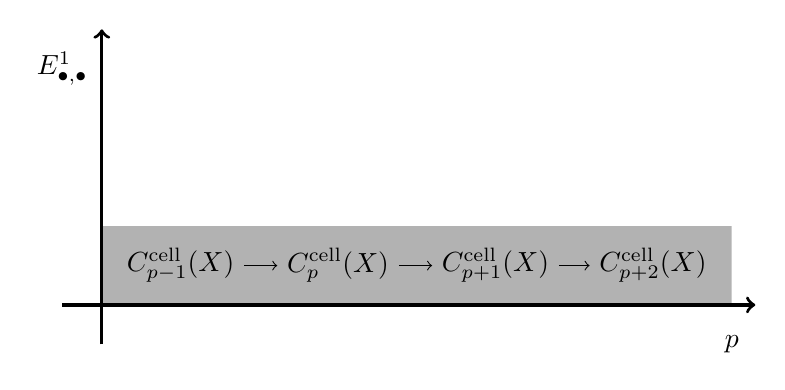
\begin{tikzpicture}
			\fill[opacity=0.3] (-1,-0.5) -- (-1,0.5) -- (7,0.5) -- (7,-0.5) -- (-1,-0.5);
			\draw[very thick, ->] (-1.5, -0.5) -- (7.3,-0.5);
			\draw[very thick, ->] (-1,-1) -- (-1,3);
			\draw 
%			(0,2) node(A){$E^{s,t}$} (2,2) node(C){$E^{s+1,t}$} (4,2) node{$\ast$} (6,2) node{$\ast$}
%			(0,1) node{$\ast$} (2,1) node{$\ast$} (4,1) node(D){$E^{s+2,t-1}$} (6,1) node{$\ast$}
			(0,0) node(A){$C_{p-1}^{\mathrm{cell}}(X)$} (2,0) node(B){$C_{p}^{\mathrm{cell}}(X)$} (4,0) node(C){$C_{p+1}^{\mathrm{cell}}(X)$} (6,0) node(D){$C_{p+2}^{\mathrm{cell}}(X)$};
			\draw 
			(-1.5,2.5) node{$E^{1}_{\bullet,\bullet}$} (7,-1) node{$p$};
			
			\draw[->] (A) --node[anchor=south]{$\de$} (B);
			\draw[->] (B) --node[anchor=south]{$\de$} (C);
			\draw[->] (C) --node[anchor=south]{$\de$} (D);
			
		\end{tikzpicture}
		\caption{La prima pagina della successione 
		spettrale nella \hyperref[h-cell]{Proposizione~\ref{h-cell}}.}
    	\label{cell-e1}
	\end{figure}
	\end{proof}
\end{prop}

\begin{ex!}[\textbf{Bicomplessi}]
	Alcuni oggetti che permettono di generare successioni spettrali come
	spiegato nel \hyperref[SS-machine]{Teorema~\ref{SS-machine}}
	sono i \emph{bicomplessi}.
	\begin{df}
		Un \textbf{bicomplesso} $(M,d^{h},d^{v})$ (o \textbf{complesso doppio})
		è un $R$-modulo bigraduato $M_{\bullet,\bullet}$
		dotato di due differenziali
		\begin{equation*}
			d^{h}_{p,q}: M_{p,q} \longrightarrow M_{p-1,q}\,, \quad
			d^{v}_{p,q}: M_{p,q} \longrightarrow M_{p,q-1}\,,
		\end{equation*}
		di bigrado $(0,-1)$ e $(-1,0)$ rispettivamente\footnote{Quello definito è un bicomplesso con notazione omologica; è facile adattare la definizione al caso coomologico considerando differenziali di bigrado $(0,1)$ e $(1,0)$ rispettivamente.},
		tali che $d^{h}d^{v} + d^{v}d^{h}=0$, ovvero ogni quadrato della griglia
		è \emph{anticommutativo}.
		\begin{equation*}
			\begin{tikzcd}
      & \dots \arrow[d]                        & \dots \arrow[d]                              &                 \\
\dots & {M_{p-1,q}} \arrow[d, "d^v"] \arrow[l] & {M_{p,q}} \arrow[d, "d^v"] \arrow[l, "d^h"'] & \dots \arrow[l] \\
\dots & {M_{p-1,q-1}} \arrow[d] \arrow[l]      & {M_{p,q-1}} \arrow[l, "d^h"] \arrow[d]       & \dots \arrow[l] \\
      & \dots                                  & \dots                                        &                
\end{tikzcd}
		\end{equation*}
		Dato un bicomplesso $M$, il suo \textbf{complesso totale} $\cat{tot}(M)$
	è l'$R$-modulo graduato dato da
	\begin{equation*}
		\cat{tot}(M)_{n} := \bigoplus_{p \in \Z} M_{s,n-s}\,,
	\end{equation*}
	dotato del \textbf{differenziale totale} $d = d^{v} + d^{h}$.
	\end{df}
	
	Quando ci viene dato un bicomplesso $M$, possiamo calcolare la sua omologia
	lungo due diverse direzioni: infatti, abbiamo l'omologia \emph{orizzontale}
	$H^{I}_{*,*}(M) := H(M_{\bullet, \bullet}, d^{h})$
	e l'omologia \emph{verticale} $H^{II}_{*,*}(M) := H(M_{\bullet, \bullet}, d^{v})$.
	La condizione $d^{h}d^{v} + d^{v}d^{h}=0$ che definisce il bicomplesso
	garantisce che il differenziale $d^{v}$ induce un differenziale verticale
	$\overline{d^{v}}$ su $H^{I}_{*,*}(M)$; analogamente, anche
	$H^{II}_{*,*}(M)$ ottiene un differenziale $\overline{d^{h}}$.
	Possiamo dunque calcolare nuovamente l'omologia di questi due complessi
	e ottenere così
	\begin{equation*}
		H^{II}_{*,*}H^{I}(M) := H\left(H^{I}_{*,*}(M), \overline{d^{v}}\right)\,, \quad
		H^{I}_{*,*}H^{II}(M) := H\left(H^{II}_{*,*}(M), \overline{d^{h}}\right)\,.
	\end{equation*}
	Questi due procedimenti danno due diverse successioni spettrali,
	le quali sono legate a $H_{*}(\cat{tot}(M))$ come spiegato nel seguente
	
	\begin{thm}\label{SS-bicomplex}
		Dato un bicomplesso $(M,d^{h},d^{v})$, esistono due successioni
		spettrali $\{ {}^{I}E^{r}_{\bullet,\bullet}, {}^{I}d^{r}\}$
		e $\{ {}^{II}E^{r}_{\bullet,\bullet}, {}^{II}d^{r}\}$, tali che
		\begin{equation*}
			 {}^{I}E^{2}_{\bullet,\bullet} \simeq H^{I}_{*,*}H^{II}(M) \,,
			 \quad  {}^{II}E^{2}_{\bullet,\bullet} \simeq H^{II}_{*,*}H^{I}(M)\,.
		\end{equation*}
		Se $M$ è concentrato nel primo quadrante, allora entrambe le successioni
		sopra convergono a $H_{*}(\cat{tot}(M))$.
		\begin{proof}
			È sufficiente dimostrare il Teorema per 
			$\{ {}^{I}E^{r}_{\bullet,\bullet}, {}^{I}d^{r}\}$,
			dato che l'altro caso è simmetrico. 
			L'idea è quella di sfruttare il \hyperref[SS-machine]{Teorema~\ref{SS-machine}}
			con $A = \cat{tot}(M)$ e $d$ il suo differenziale totale. 
			Definiamo quindi le filtrazioni sul complesso totale
			\begin{equation*}
				F^{I}_{p}\left( \cat{tot}(M) \right)_{q} := \bigoplus_{r \le p} M_{r,q-r}\,,
				\quad
				F^{II}_{p}\left( \cat{tot}(M) \right)_{q} := \bigoplus_{r \le p} M_{q-r,r}\,,
			\end{equation*}
			dove $F^{I}$ viene detta \textbf{filtrazione per colonne},
			mentre $F^{II}$ viene detta \textbf{filtrazione per righe}.
			
			\missingfigure{Add image of filtration}
			
			Per prima cosa identifichiamo la prima pagina della successione:
			notiamo che per ogni $p,q \in \Z$ la filtrazione dà il quoziente
			\begin{equation*}
					\left( \frac{F_{p}^{I}(\cat{tot}(M))}{F_{p-1}^{I}(\cat{tot}(M))} \right)_{p+q}
					=  \frac{\bigoplus_{r \le p} M_{r, p + q - r}}{\bigoplus_{r \le p-1} M_{r,p+q-r}}
					% \simeq \left( M_{p,\bullet} \right)_{p+q}
					\simeq M_{p,q}\,,
			\end{equation*}
			quindi la tripla $\big(F^{I}_{p}(\cat{tot}(M)), F^{I}_{p-1}(\cat{tot}(M)), 
			F^{I}_{p-2}(\cat{tot}(M))\big)$ dà la successione esatta di complessi
			\begin{equation*}
				\begin{tikzcd}
					\cat{0} \ar[r]
					& M_{p-1,\bullet} \ar[r]
					& M_{p-1,\bullet} \oplus M_{p,\bullet} \ar[r]
					& M_{p,\bullet} \ar[r]
					& \cat{0}\,,
				\end{tikzcd}
			\end{equation*}
			ognuno dei quali è dotato del \emph{differenziale verticale} $d^{v}$,
			quindi grazie al \textbf{Lemma del Serpente} si ottiene
			\begin{equation*}
				\begin{tikzcd}[column sep=small]
					\dots \ar[r]
					& H_{p+q}(M_{p,\bullet}, d^{v}) = H^{II}_{p,q}(M) \ar[r, "\delta"]
					& H_{p+q-1}(M_{p-1,\bullet}, d^{v}) = H^{II}_{p-1,q}(M) \ar[r]
					& \dots
				\end{tikzcd}
			\end{equation*}
			dove si verifica che $\delta = \overline{d^{h}}$. Si deduce quindi che
			${}^{I}E_{\bullet,\bullet}^{1} \simeq H^{II}_{*,*}(M)$, 
			da cui si conclude che
			\begin{equation*}
				{}^{I}E_{\bullet,\bullet}^{2} \simeq H^{I}_{*,*}H^{II}(M)\,.
			\end{equation*}
			
			Infine, se $M$ è concentrato nel primo quadrante, 
			la filtrazione $F^{I}$ è limitata sia dal basso, sia dall'alto,
			dato che per ogni $t \in \Z$ vale
			\begin{equation*}
				\cat{tot}(M)_{t} =  F^{I}_{t}\cat{tot}(M)_{t} 
				\supset F^{I}_{t-1}\cat{tot}(M)_{t}
				\supset \dots \supset F^{I}_{0}\cat{tot}(M)_{t} 
				= M_{0,t} \supset F^{I}_{-1}\cat{tot}(M)_{t}  = 0\,,
			\end{equation*}			
			quindi per il \hyperref[SS-machine]{Teorema~\ref{SS-machine}}
			la successione converge a $H(\cat{tot}(M))$.
%			\begin{equation*}
%				\frac{F_{p}H_{p+q}(\cat{tot}(M))}{F_{p-1}H_{p+q}(\cat{tot}(M))}
%				=  \frac{\bigoplus_{r \le p} M_{r, p + q - r}}{\bigoplus_{r \le p-1} M_{r,p+q-r}}
%					% \simeq \left( M_{p,\bullet} \right)_{p+q}
%					\simeq H_{p+q}(\cat{tot}(M))\,.
%			\end{equation*}
		\end{proof}
	\end{thm}
\end{ex!}

\begin{ex!}[\textbf{Formula di Künneth}]
	Dati $(C_{\bullet},d)$ e $(D_{\bullet},\de)$ due complessi di catene su un campo $\KK$,
	consideriamo il bicomplesso $C_{\bullet} \otimes D_{\bullet}$ avente i differenziali
	\begin{equation*}
		d^{h}(x \otimes y) := dx \otimes y\,, \quad 
		d^{v}(x \otimes y) := (-1)^{\lvert x \rvert} x \otimes \de y\,.
	\end{equation*}
	Il suo complesso totale $T_{\bullet} := 
	\cat{tot}\left( C_{\bullet} \otimes D_{\bullet} \right)$
	è quindi dotato del differenziale
%	allora per ogni $n \in \Z$ vale
%	\begin{equation}\label{kunneth}
%		H_{n}\left( C_{\bullet} \otimes D_{\bullet} \right)
%		= \left( H_{*}(C_{\bullet}) \otimes H_{*}(D_{\bullet}) \right)_{n}\,.
%	\end{equation}
%	\begin{proof}
%		Ricordiamo che $T_{\bullet} := C_{\bullet} \otimes D_{\bullet}$ è
%		il complesso di catene dato in grado $q$ da
%		\begin{equation*}
%			T_{q} = \bigoplus_{i+j=q}C_{i} \otimes_{\KK} D_{j}\,,
%		\end{equation*}
%		dotato del differenziale
		\begin{equation*}
			D(x \otimes y) := dx \otimes y + (-1)^{\lvert x \rvert} x \otimes \de y \,,
		\end{equation*}
		e se si considera la filtrazione per colonne su $T_{\bullet}$, 
		data da
		\begin{equation*}
			F_{p}^{I}(T_{q}) := \bigoplus_{r \le p} C_{i} \otimes_{\KK} D_{q-r}\,,
		\end{equation*}
		allora per il \hyperref[SS-bicomplex]{Teorema~\ref{SS-bicomplex}}
		sappiamo che la successione spettrale associata converge a $H_{*}(T_{\bullet})$.
		Studiamo dunque le prime pagine della successione:
		la $0$-esima pagina è definita da $E^{0}_{p,q} := C_{p} \otimes_{\KK} D_{q}$,
		con differenziale $d^{0} := (-1)^{p} \cat{1}_{C} \otimes \de$,
		quindi si ottiene $E^{1}_{p,q} = C_{p} \otimes_{\KK} H_{q}(D_{*})$.
		Segue dal \hyperref[SS-machine]{Teorema~\ref{SS-machine}} che
		il differenziale $d^{1} = d \otimes \cat{1}_{H_{*}(D)}$,
		quindi la seconda pagina sarà 
		$E^{2}_{p,q} = H_{p}(C_{\bullet}) \otimes H_{q}(D_{\bullet})$
		con differenziali tutti nulli.
		Dato che $E_{\bullet,\bullet}^{2} = E_{\bullet, \bullet}^{\infty}$, 
		allora si ottiene la \textbf{Formula di Künneth}
	\begin{equation}\label{kunneth}
		H_{n}\left( C_{\bullet} \otimes D_{\bullet} \right)
		= \bigoplus_{p+q=n} H_{p}(C_{\bullet}) \otimes_{\KK} H_{q}(D_{\bullet}) 
		= \big(  H_{*}(C_{\bullet}) \otimes H_{*}(D_{\bullet}) \big)_{n} \,.
	\end{equation}
%	\end{proof}
\end{ex!}

\begin{ex!}[\textbf{Complesso di \v{C}ech-de Rham}]
	Dimostriamo che esiste un isomorfismo tra la 
	\textbf{coomologia di \v{C}ech} e la \textbf{coomologia di de Rham}
	di una varietà differenziabile reale. 
	Ricordiamo prima alcune nozioni:
	
	\begin{df}
		Data $M$ una varietà differenziabile reale,
		denotiamo con $\Omega^{k}(M)$ lo spazio delle $k$-forme
		$C^{\infty}$ su $M$, cioè lo spazio delle sezioni $C^{\infty}$
		del fibrato $\bigwedge^{k} T^{*}M$.
	\end{df}
	
	Ricordiamo che un elemento
		$\alpha \in \Omega^{k}(M)$ su un aperto coordinato
		è della forma
		\begin{equation*}
			\alpha = \sum_{|I| = k} \alpha_{I}(x) dx_{I}\,,
		\end{equation*}
		con $I$ il $k$-multiindice che rappresenta $i_{1} \le i_{2} \le \dots \le i_{k}$
		e $dx_{I} = dx_{i_{1}} \wedge dx_{i_{2}} \wedge \dots \wedge dx_{i_{k}}$.
		Localmente definiamo il \textbf{differenziale esterno} 
		$d : \Omega^{k}(M) \to \Omega^{k+1}(M)$ con la formula
		\begin{equation*}
			d\alpha = \sum_{j=1}^{n}\sum_{|I|=k} \frac{\de \alpha_{I}}{\de x_{j}}(x) \, 
			dx_{j} \wedge dx_{I}
		\end{equation*}
		e otteniamo il \textbf{complesso di de Rham} $(\Omega^{\bullet}(M),d)$,
		la cui coomologia sarà indicata con $H^{*}_{\mathrm{dR}}(M)$.
	
	\begin{lemma**}[Poincarè]
		Ogni forma chiusa su un aperto contraibile $A \subset \R^{n}$ è esatta.
		In altri termini, se $A$ è contraibile allora vale
		\begin{equation*}
			H^{k}_{\mathrm{dR}}(A) \simeq
			\begin{cases}
				\R\,, \quad &\text{se } k=0\,;\\
				0\,, \quad &\text{se } k>0\,.
			\end{cases}
		\end{equation*}
	\end{lemma**}
		
		Sia $M$ una varietà differenziabile e $\Uu$ un ricoprimento di $M$.
		Per una $k$-upla $U_{i_{1}}, \dots, U_{i_{k}} \in \Uu$, 
		indichiamo con $U_{i_{1}, \dots, i_{k}} := U_{i_{1}} \cap \dots \cap U_{i_{k}}$.
		
	\begin{df}
		Il \textbf{complesso di \v{C}ech a coefficienti reali} per $(M,\Uu)$ 
		è dato dagli $\R$-spazi vettoriali
		\begin{equation*}
			\v{C}_{\Uu}^{k}(M) := \bigoplus_{i_{0} \le \dots \le i_{k}} \underline{\R}(U_{i_{0}, \dots, i_{k}})\,,
		\end{equation*}
		dove $\underline{\R}$ è il fascio delle funzioni reali localmente costanti,
		sui quali definiamo i differenziali
		\begin{equation*}
			\delta^{k}: \v{C}^{k}_{\Uu}(M) \to \v{C}^{k+1}_{\Uu}(M)\,, \quad
			(\delta^{k}\alpha)_{i_{0}, \dots, i_{k+1}} :=
			\sum_{j=0}^{k+1} (-1)^{j} \alpha_{i_{0} \dots \hat{i_{j}} \dots i_{k+1}}\,.
		\end{equation*}
		Definiamo la \textbf{coomologia di \v{C}ech} subordinata al ricoprimento $\Uu$
		come
		\begin{equation*}
			\check{H}^{*}(M, \Uu) := H^{*}\left( \v{C}^{\bullet}_{\Uu}(M), \delta \right) \,.
		\end{equation*}
	\end{df}		
	
	Chiamiamo $\Uu$ un \textbf{buon ricoprimento} di $M$ se ogni aperto $U_{i} \in \Uu$
	è contraibile e ogni intersezione finita di aperti di $\Uu$ è vuota oppure contraibile.
		
	\begin{thm}
		Sia $M$ una $n$-varietà reale $C^{\infty}$ e $\Uu$ un buon ricoprimento per $M$.
		Allora la coomologia di \v{C}ech su $\Uu$ coincide con quella di De Rham,
		cioè esiste un isomorfismo naturale
		\begin{equation*}
			\check{H}^{*}(M;\Uu) \simeq H^{*}_{\mathrm{dR}}(M)\,.
		\end{equation*} 
		\begin{proof}
			Definiamo il \emph{complesso doppio di \v{C}ech-de Rham} come
			\begin{equation*}
				C^{p,q} := \prod_{i_{0} \le i_{1} \le \dots \le i_{p}} \Omega^{q}(U_{i_{0} \dots i_{p}})\,;
			\end{equation*}
%			su cui consideriamo il differenziale $D := \delta + (-1)^{p}d$.
			la pagina $E_{0}^{\bullet, \bullet}$ appare così:
			\begin{equation*}
				\begin{tikzcd}[column sep=small]
					\dots & & & \\
					\prod_{i_{0}} \Omega^{2}(U_{i_{0}}) \ar[r] \ar[u]
					&  \dots & & \\
					\prod_{i_{0}} \Omega^{1}(U_{i_{0}}) \ar[r, "\delta"] \ar[u, "d"] 
					& \prod_{i_{0} \le i_{1}} \Omega^{1}(U_{i_{0} i_{1}})  \ar[u, "d"] \ar[r] & \dots  & \\
					\prod_{i_{0}} \Omega^{0}(U_{i_{0}}) \ar[r, "\delta"] \ar[u, "d"] 
					& \prod_{i_{0} \le i_{1}} \Omega^{0}(U_{i_{0} i_{1}})  \ar[u, "d"] \ar[r] & 
					\prod_{i_{0} \le i_{1} \le i_{2}} \Omega^{0}(U_{i_{0} i_{1} i_{2}})  
					\ar[u] \ar[r] & \dots
				\end{tikzcd}
			\end{equation*}
			Prendiamo dunque il complesso totale $T^{\bullet}$ associato al bicomplesso,
			cioè
			\begin{equation*}
				T^{n} := (\cat{tot} \, C)_{n} = \bigoplus_{p+q=n} C^{p,q}\,,
			\end{equation*}
			con differenziale $D = \delta + (-1)^{p}d$, sul quale consideriamo due
			diverse filtrazioni:
			\begin{itemize}
				\item la filtrazione per colonne 
				$F^{p}_{I}T^{n} := \bigoplus_{r \ge p} T^{r,n-r}$
				induce su $E_{0}^{p,q} = C^{p,q}$ il
				differenziale $d_{0} = (-1)^{p}d$, quindi per
				il \hyperref[SS-bicomplex]{Teorema~\ref{SS-bicomplex}}
				la prima pagina è data da
				\begin{equation*}
				E_{1}^{p,q} 
				= H_{II}^{p,q}(C) 
				= \prod_{i_{0} \le \dots \le i_{p}} H_{\mathrm{dR}}^{q}(U_{i_{0} \dots i_{p}})
				= \begin{cases}
					\R\,, \quad &\text{se } q = 0\,; \\
					0\,, \quad &\text{altrimenti},
				\end{cases}
				\end{equation*}
				dove l'ultima uguaglianza segue dall'ipotesi di $\Uu$ buon ricoprimento.
				Si noti in particolare che
				\begin{equation*}
					H^{0}_{\mathrm{dR}}(U_{i_{0} \dots i_{p}}) 
					= \R
					= \underline{\R}(U_{i_{0} \dots i_{p}})
				\end{equation*}
				è dotato del differenziale  $d_{1}=\delta$. Dato che la successione
				collassa alla seconda pagina, 
				il limite è $E_{\infty}^{p,q} = E_{2}^{p,q}$,
				quindi si conclude che
				\begin{equation*}
				 	H^{*}(T^{bullet}) = \check{H}^{*}(M;\Uu)\,.
				 \end{equation*}
				
				\item Dalla filtrazione per righe 
				$F_{II}^{p}C^{n}=\bigoplus_{r \ge p} C^{n-r,r}$
				si ottiene $E_{0}^{p,q} = C^{p,q}$ con il differenziale $d_{0}=\delta$.
				
				\begin{lemma}
					C'è un'omotopia di catene
					\begin{equation*}
						\kappa : \prod_{i_{0} \le \dots \le i_{p}} \Omega^{\bullet} (U_{i_{0} \dots i_{p}})
						\longrightarrow \prod_{i_{0} \le \dots \le i_{p-1}} \Omega^{\bullet} (U_{i_{0} \dots i_{p-1}})
					\end{equation*}
					tra l'identità e la mappa nulla in grado $p > 0$.
					\begin{proof}
						Data $\{\rho_{i}\}_{i}$ una partizione dell'unità
						sbordinata a $\Uu$, 
						è sufficiente porre
						\begin{equation*}
							(\kappa \omega)_{i_{0} \dots i_{p-1}} 
							:= \sum_{i} \rho_{i} \, \omega_{i\,i_{0} \dots i_{p-1}}\,.
						\end{equation*}
						Infatti si verifica che per ogni $p > 0$ si ha
						\begin{align*}
							(\delta \kappa \omega)_{i_{0} \dots i_{p}}
							=& \sum_{j = 0}^{p} \sum_{i} (-1)^{j} \rho_{i} \, \omega_{i\,i_{0} \dots \hat{i_{j}} \dots i_{p}}\,, \\
							(\kappa \delta \omega)_{i_{0} \dots i_{p}}
							= \omega_{i_{0} \dots i_{p}} +& \sum_{i} \sum_{j = 0}^{p} (-1)^{j+1} \rho_{i} \, \omega_{i\,i_{0} \dots \hat{i_{j}} \dots i_{p}}\,,
						\end{align*}
						quindi $\delta \kappa + \kappa \delta = \cat{1}$.
					\end{proof}
				\end{lemma}
				
				Come conseguenza di questo \textbf{Lemma}, 
				segue che in $E^{p,q}_{1}$
				sopravvive solo la colonna $p=0$.
				Dato che $\ker \delta$ è costituito dalle $k$-forme \emph{globali},
				allora 
				\begin{equation*}
				E_{1}^{p,q} 
				= \begin{cases}
					\Omega^{q}(M) \,, \quad &\text{se } p = 0\,; \\
					0\,, \quad &\text{altrimenti},
				\end{cases}
				\end{equation*}
				e si verifica che il differenziale verticale è $d_{1}=d$ qdi de Rham.
				La successione collassa alla seconda pagina, per cui si ha
				\begin{equation*}
					E_{\infty}^{p,q} = E_{2}^{p,q}
					= \begin{cases}
						H_{\mathrm{dR}}^{q}(M)\,, \quad \text{se } p=0\,; \\
						0\,, \quad \text{altrimenti},
					\end{cases}
				\end{equation*}
				quindi concludiamo che $H^{*}(T^{\bullet}) = H_{\mathrm{dR}}^{*}(M)$.
			\end{itemize}
			Ricapitolando, abbiamo dimostrato che 
			$\check{H}^{*}(M;\Uu) = H^{*}(T^{\bullet}) = H_{\mathrm{dR}}^{*}(M)$.
		\end{proof}
	\end{thm}
\end{ex!}






%	 %%% Lezione 14


\lecture[Successione spettrale e successione della coppia. Fibrati di Serre e teorema sulla successione spettrale di omologia associata ad un fibrato di Serre. Applicazione al calcolo dell'omologia di alcuni gruppi $SU(n)$. Applicazione al calcolo di alcuni gruppi di omologia dello spazio dei loop su uno spazio $X$ $n$-connesso.]{2023-04-18}

\begin{ex}[\textbf{Successione di una coppia}]
	Data una  coppia di spazi $(X,Y)$, possiamo considerare
	l'inclusione $i : Y \subset X$ come una filtrazione	
	\begin{equation*}
		 X_{-1} \subset X_{0} \subset X_{1}\,,
	\end{equation*}
	dove $X_{-1} = \emptyset, X_{0}=Y$ e $X_{1}=X$.
	Questa % filtrazione
	determina la filtrazione $C_{*}(Y) \subset C_{*}(X)$ 
	sulle catene singolari di $X$,
	dalla quale otteniamo la successione spettrale
	\begin{equation}\label{SS-coppia}
		E^{1}_{p,q} = H_{p+q}(X_{p},X_{p-1}) = 
		\begin{cases}
			H_{q}(Y) \,, \quad &\text{se } p=0\,; \\
			H_{q+1}(X,Y) \,, \quad &\text{se } p=1\,\\
			0\,, \quad &\text{altrimenti.}
		\end{cases}
	\end{equation}
	\missingfigure{Fai disegno}
	Si può verificare che la mappa di bordo sulla prima pagina
	\begin{equation*}
		d^{1}: E^{1}_{1,q} \longrightarrow E^{1}_{0,q}\,,
	\end{equation*}
	coincide con l'omomorfismo di connessione della coppia
	\begin{equation*}
		\de : H_{q+1}(X,Y) \longrightarrow H_{q}(Y)\,.
	\end{equation*}
	
	Viceversa, supponiamo di avere il dato della successione spettrale
	$(E^{1}_{\bullet, \bullet}, d^{1})$;
	vogliamo ricostruire la successione della coppia.
	Dato che la prima pagina si concentra in due
	colonne adiacenti, è chiaro che la successione 
	collassa alla seconda pagina,
	quindi il termine limite è $E^{\infty}_{\bullet,\bullet} = E^{2}_{\bullet,\bullet}$.
	Per il \hyperref[SS-machine]{Teorema~\ref{SS-machine}},
	calcoliamo il limite per $p=0$ come
	\begin{equation*}
		E^{\infty}_{0,q} = \frac{F_{0}H_{*}}{F_{-1}H_{*}}
		= \frac{\im \left( H_{q}(Y) \to H_{q}(X) \right)}{\im \left( H_{q}(\emptyset) \to H_{q}(X) \right)}
		= \im \left(H_{q}(Y) \xrightarrow{i^{*}} H_{q}(X) \right)\,,
	\end{equation*}
	mentre sulla prima colonna è dato da
	\begin{equation*}
		E^{\infty}_{1,q} = \frac{H_{q+1}(X)}{\im \left( i_{*}: H_{q+1}(Y) \to H_{q+1}(X) \right)}\,.
	\end{equation*}
	D'altra parte la seconda pagina è data da
	\begin{align*}
		E^{2}_{1,q} 
		= \ker \left( H_{q+1}(X,Y) \xrightarrow{\de} H_{q}(Y) \right) \,, \quad
		E^{2}_{0,q} 
		= \frac{H_{q}(Y)}{\im \de} \,.
	\end{align*}
	Confrontando $E^{\infty}$ con la pagina $E^{2}$ si hanno le identità
	\begin{align*}
		E^{2}_{1,q} 
		&= \ker \left( H_{q+1}(X,Y) \xrightarrow{\de} H_{q}(Y) \right) 
		= \frac{H_{q+1}(X)}{\im \left(  H_{q+1}(Y) \to H_{q+1}(X) \right)}
		= E^{\infty}_{1,q}\,, \\
		E^{2}_{0,q} 
		&= \frac{H_{q}(Y)}{\im \de} 
		= \im \left(  H_{q}(Y) \xrightarrow{i^{*}} H_{q}(X) \right)
		= E^{\infty}_{0,q}\,.
	\end{align*}
	dalle quali si ottiene la successione esatta
	\begin{equation*}
		\begin{tikzcd}[column sep=small]
			\cat{0} \ar[r]
			& \frac{H_{q}(Y)}{\im \left(  H_{q+1}(X,Y) \to H_{q}(Y) \right)} \ar[r]
			& H_{q}(X) \ar[r]
			&  \ker \left( H_{q}(X,Y) \xrightarrow{\de} H_{q-1}(Y) \right) \ar[r]
			& \cat{0}\,,
		\end{tikzcd}
	\end{equation*}
	per ogni $q \in \Z$, 
	ovvero la successione della coppia $(X,Y)$.
	Ne segue che la successione della coppia è equivalente alla successione spettrale
	\eqref{SS-coppia}.
\end{ex}




\section{Successioni spettrali di Serre}

Ricordiamo la seguente definizione.

\begin{df}
	Una mappa $\pi : E \to B$ è una \textbf{fibrazione di Serre} se
	vale la \eqref{HLP} sui cubi:
	\begin{equation}\label{Serre-HLP}
		\begin{tikzcd}
			I^{n} \times \{0\} \ar[r] \ar[d, "\iota_{0}"', hook] & E \ar[d, "\pi"] \\
			I^{n+1} \ar[r] \ar[ur, dashed] & B\,. \tag{HLP'}
		\end{tikzcd}
	\end{equation}
\end{df}

Se $B$ è uno spazio connesso per archi che ammette un rivestimento universale $\widetilde{B}$,
allora per il \textbf{Teorema di approssimazione} possiamo trovare un'equivalenza
omotopica debole $f: B' \to B$, con $B'$ un CW complesso. Siccome le fibrazioni
sono una classe chiusa per pullback (vedi \hyperref[fib-prop]{Esercizio~\ref{fib-prop}}), 
allora anche $f^{*}E \to B'$ 
è una fibrazione di Serre, pertanto assumeremo 
senza perdita di generalità che la \emph{base $B$ sia un CW complesso}.

Fissato $x \in B$, consideriamo  $E_{x} = \pi^{-1}(x)$ e
a questa fibra associamo $H_{*}(E_{x})$. 
Adesso vorremmo associare un omomorfismo 
$\gamma_{*} : H_{*}(E_{x}) \to H_{*}(E_{x'})$
per ogni cammino
$\gamma : x \to x'$ in $B$. 
Presa $\alpha_{0} : A_{x} \to E_{x}$ un'approssimazione CW della fibra su $x$,
possiamo usare la \eqref{Serre-HLP} induttivamente sullo scheletro di $A_{x}$
per poter sollevare l'omotopia 
\begin{equation*}
	\Gamma: A_{x} \times I \longrightarrow B\,, \quad
	\Gamma(z,t) := \gamma(t)\,,
\end{equation*}
per ottenere così una mappa diagonale
\begin{equation*}
	\begin{tikzcd}
		A_{x} \times \{0\} \ar[r, "\alpha_{0}"] \ar[d, "\iota_{0}"', hook] & E \ar[d, "\pi"] \\
		A_{x} \times I \ar[r] \ar[ur, dashed, "\alpha"] & B\,. 
	\end{tikzcd}
\end{equation*}
Allora $\alpha_{1} :A_{x} \to E_{x'}$ induce in omotopia un omomorfismo
$\gamma_{*} : H_{*}(E_{x}) \to H_{*}(E_{x'})$.
Notiamo inoltre che se $\gamma \sim \gamma'$ sono omotopi \emph{a estremi fissati},
allora producono lo stesso omomorfismo in omologia; in particolare,
se $x=x'$, notiamo allora che $\pi_{1}(B,x)$ agisce su
$H_{*}(E_{x})$ e si verifica che $\gamma$ è costante induce $\gamma_{*} = \cat{1}_{H_{*}(E_{x})}$.
Questo appena descritto è un esempio di \emph{sistema locale}.

\begin{df}
	Un \textbf{sistema locale di gruppi} $\Gg = \Set{G_{x},\tau_{\gamma}}$ 
	su uno spazio topologico $X$ è un funtore che associa a ogni punto $x \in X$
	un gruppo $G_{x}$ e a ogni cammino $\gamma : I \to X$ da $x_{0}$ a $x_{1}$
	associa un omomorfismo
	\begin{equation*}
		\tau_{\gamma} : G_{x_{0}} \longrightarrow G_{x_{1}}
	\end{equation*}
	che dipende solamente dalla classe
	\begin{equation*}
		[\gamma] \in [(I, \de I) ; (X, \{x_{0}, x_{1} \})]\,,
	\end{equation*}
	con la condizione che se $\gamma$ è costante in $x$, 
	allora l'omomorfismo associato è $\tau_{\gamma} = \cat{1}_{G_{x}}$.
\end{df}

\begin{oss}
	Il gruppo fondamentale $\pi_{1}(B,x)$ agisce (da \emph{sinistra})
	sul gruppo $G_{x}$.
\end{oss}


\begin{oss}
	Siccome ogni cammino $\gamma$ può essere ripercorso in senso
	contrario e produrre il cammino opposto $\overline{\gamma}$
	in modo che la composizione $\gamma \overline{\gamma}$ sia omotopo a una costante,
	deduciamo che ogni $\tau_{\gamma}$ è un isomorfismo.
	In particolare, se $X$ è connesso per archi, allora tutti i $G_{x}$
	di un sistema locale sono isomorfi.
\end{oss}

\begin{df}
	Se l'azione di $\pi_{1}(B,x)$ su $G_{x}$ è banale,
	allora diremo che il sistema locale $\Gg$ è \textbf{banale}.
\end{df}

\begin{ex}
	Ogni sistema locale su uno spazio semplicemente connesso è banale.
\end{ex}


Supponiamo ora che $X$ sia uno spazio connesso per archi
che ammette rivestimento universale $\widetilde{X}$.
Allora $\pi_{1}(X,x_{0})$ agisce (da \emph{destra})
su $\widetilde{X}$ per \textbf{traslazione}, ovvero
\begin{equation*}
	\widetilde{X} \times \pi_{1}(X,x_{0})\,, \quad
	(x,\gamma) \longmapsto x'
\end{equation*}
dove $x'$ è \todo{noccapito}

In particolare questo induce un'azione \emph{destra} di $\pi_{1}(X,x_{0})$
sulle catene singolari $C_{*}(\widetilde{X})$ per traslazione,
e si verifica che questa azione commuta con il differenziale $d$.

\begin{df}
	Dato $x_{0}$ in $X$ connesso per archi, il complesso
	\begin{equation*}
		C_{*}(X;\Gg) := C_{*}(\widetilde{X}) \otimes_{\Z[\pi_{1}(X,x_{0})]} G_{x_{0}}
	\end{equation*}
	viene chiamato \textbf{complesso delle catene singolari a coefficienti in $\Gg$},
	il cui bordo è indotto da $d:C_{*}(\widetilde{X}) \to C_{*}(\widetilde{X})$.
	Passando al duale, definiamo le \textbf{cocatene singolari a coefficienti in $\Gg$}
	come
	\begin{equation*}
		C^{*}(X;\Gg) := \Hom_{\Z[\pi_{1}(X,x_{0})]}\left(C_{*}(\widetilde{X};G_{x_{0}}\right)\,.
	\end{equation*}
	L'\textbf{omologia}, risp. la \textbf{coomologia}, a coefficienti
	in un sistema locale $\Gg$ sarà indicata con
	\begin{equation*}
		H_{*}(X;\Gg) := H_{*}(C_{*}(X;\Gg))\,, \quad
		\text{resp. } H^{*}(X;\Gg) := H^{*}(C^{*}(X;\Gg))\,.
	\end{equation*}
\end{df}


\begin{thm}[\textbf{Successione spettrale di Serre}]\label{Serre-SS}
	Sia $M$ uno $\Z$-modulo.\todo{Oppure modulo su un qualunque anello?}	
	Data una fibrazione di Serre $\pi:E \to B$,
	esiste una successione spettrale $\Set{(E^{r}_{p,q},d^{r})}_{r \ge 2}$
	concentrata nel primo quadrante data da
	\begin{equation*}
		E_{p,q}^{r} = H_{p}\left(B; \Set{H_{q}(E_{x};M)}\right)\,,
	\end{equation*}
	convergente a $E^{\infty}_{p,q} = F_{p}H_{p+q}(E;M)$,
	per una qualche filtrazione $F$ dell'omologia 
	$H_{*}(E;M)$.
\end{thm}

\begin{oss}
	Si noti che nel \hyperref[Serre-SS]{Teorema~\ref{Serre-SS}}
	non vengono nemmeno citati i differenziali della successione spettrale!
\end{oss}

Prima di dimostrare questo risultato,
vediamo alcuni esempi per capirne il funzionamento.

\begin{ex}
	Sia $SU(n)$ il gruppo delle matrici complesse unitarie con determinante $1$.
	Ad esempio, per $n=2$ abbiamo
	\begin{equation*}
		SU(2) : \Set{ \begin{bmatrix} \alpha & \beta \\ \overline{\beta} & \overline{\alpha} \end{bmatrix}	
		| {|alpha|}^{2}	+ {|\beta|}^{2} = 1 }
		\simeq S^{3}\,.
	\end{equation*}
	La topologia di $SU(3)$ invece è più complicata
	e usiamo il \hyperref[Serre-SS]{Teorema~\ref{Serre-SS}}
	per studiarne l'omologia. La mappa 
	
	In maniera analoga possiamo studiare l'omologia
	di $SU(4)$, infatti presa la fibrazione
	\begin{equation*}
		SU(3) \hookrightarrow SU(4) \longrightarrow S^{7}\,,
	\end{equation*}
	otteniamo la successione spettrale la cui pagina $E^{2}_{\bullet,\bullet}$ 
	è data da
	\missingfigure{Pagina}
	e quindi concludiamo che
	\begin{equation*}
		H_{p}\left( SU(4) \right) =
		\begin{cases}
			\Z\,, \quad &\text{se } p = 0,3,5,7,8,10,12\,;\\
			0\,, \quad &\text{altrimenti.}
		\end{cases}
	\end{equation*}
	
	Infine, vorremmo studiare anche l'omologia di $SU(5)$ 
	utilizzando la fibrazione
	\begin{equation*}
		SU(4) \hookrightarrow SU(5) \longrightarrow S^{9}\,.
	\end{equation*}
	A questo punto $E^{2}_{\bullet,\bullet}$ 
	è data da
	\missingfigure{pagina con differenziali non banali}
	e notiamo che potrebbero esserci due differenziali non banali.
	Purtroppo non conosciamo la struttura di $d^{9}$,
	quindi (per ora) non sappiamo come calcolare $H_{*}\left( SU(5) \right)$.
\end{ex}

Dato uno spazio topologico $X$, ricordiamo che possiamo costruire la fibrazione
\begin{equation*}
	\begin{tikzcd}
		\Omega X \ar[r] & PX \ar[r, "ev_{1}"] & X\,,
	\end{tikzcd}
\end{equation*}
dove lo spazio dei cammini $PX$ è contraibile. 
Se supponiamo che $X$ sia $n$-connesso,
preso il sistema locale $\Set{H_{q}(P_{x_{0}}^{x}X)}$,
per il  \hyperref[Serre-SS]{Teorema~\ref{Serre-SS}} si ha
\begin{equation*}
	E^{2}_{p,q} = H_{q}(X;\Set{H_{q}(P_{x_{0}}^{x}X)})\,,
\end{equation*}
e \todo{Finire che non sto capendo}








%	 %%% Lezione 15


\lecture[Lezione 15.]{2023-04-24}

	Abbiamo ricavato nuovamente il teorema di Hurewicz
	per gruppi di omotopia superiore,
	assumendo il risultato vero solo per $\pi_{1}$.\todo{recupera}
	
	\begin{ex}
		Studiamo i loop sulla sfera $S^{n}$.
		Supponiamo che $n > 1$ così da avere la base semlicemente connessa.
		Dalla fibrazione
		\begin{equation*}
			\begin{tikzcd}
				\Omega S^{n} \ar[r] & PS^{n} \ar[r] & S^{n}
			\end{tikzcd}
		\end{equation*}
		otteniamo la successione spettrale
		\begin{equation*}
			E^{2}_{p,q} = H_{p}\big(S^{n},H_{q}(\Omega S^{n}) \big)\,.
		\end{equation*}
		La colonna $p=0$ è lo $0$-esimo gruppo di omologia di uno spazio connesso
		a coefficienti in $H_{q}(\Omega S^{n})$, quindi la prima colonna è in realtà
		l'omologia della fibra $H_{q}(\Omega S^{n})$. 
		Tutte le altre colonne hanno gruppi banali, fino a quando
		$p = n$, in cui ritroviamo l'omologia in grado $n$ di $S^{n}$
		a coefficienti in $H_{q}(\Omega S^{n})$, che è isomorfa a $\Z$ per $q=n-1$.
		\missingfigure{Devo mettere una bella pagina di sta roba.}
		
		Procedendo per induzione, questo dimostra che per ogni $k \in \N$
		l'omologia di $\Omega S^{n}$ è
		\begin{equation*}
			H_{k(n-1)}(\Omega S^{n}) \simeq \Z
		\end{equation*}
		ed è banale in tutti gli altri gradi.\todo{non ho capito la roba della formula di Künneth e il limite...}
	\end{ex}
	
	
	
	\section{Confronto di successioni spettrali}
	
	
	La costruzione del \hyperref[SS-machine]{Teorema~\ref{SS-machine}}
	che associa ad un complesso filtrato graduato $(C,d,F)$ una successione spettrale
	è \emph{funtoriale}, nel senso che un morfismo tra complessi filtrati e graduati
	induce in maniera naturale un morfismo di successioni spettrali.
	
	\begin{thm}
		Sia $\tau : C \to C'$ una mappa di complessi differenziali graduati e filtrati.
		Supponiamo che le filtrazioni in omologia 
		\begin{equation*}
			\bigcup_{s} F_{s}H_{n} = H_{n}
		\end{equation*}
		siano convergenti e limitate dal basso.
		Se per qualche $r \ge 1$ la mappa $\tau^{r} : E^{r} \to (E')^{r}$ è un isomorfismo,
		allora per tutte le pagine $t \ge r$ si ha $E^{t} \simeq (E')^{t}$ e
		la mappa in omologia
		\begin{equation*}
			\tau_{*} : H_{*}(C) \longrightarrow H_{*}(C')
		\end{equation*}
		è un isomorfismo.
		\begin{proof}
			\`E chiaro che se le successioni spettrali
			coincidono alla pagina $r$, siccome le pagine successive
			sono determinate da quelle precedenti, allora
			$\tau^{t}$ è un isomorfismo per ogni $t \ge r$.
			In particolare, anche il limite
			\begin{equation*}
				\tau^{\infty} : E^{\infty} \longrightarrow (E')^{\infty}
			\end{equation*}
			è un isomorfismo.
			
			Abbiamo un diagramma commutativo
			\begin{equation*}
				\begin{tikzcd}
					0 \ar[r]
					& F_{s-1}H_{n}(C) \ar[r] \ar[d]
					& F_{s}H_{n}(C) \ar[r] \ar[d]
					& E^{\infty}_{s,n-s} \ar[r] \ar[d]
					& 0 \\
					0 \ar[r]
					& F_{s-1}H_{n}(C') \ar[r]
					& F_{s}H_{n}(C') \ar[r]
					& (E')^{\infty}_{s,n-s} \ar[r]
					& 0 \,.
				\end{tikzcd}
			\end{equation*}
			Fissato $n$, per valori abbastanza piccoli di $s$
			si ha $F_{s-1}H_{n}(C) = 0$ e $F_{s-1}H_{n}(C')$ perché la filtrazione è limitata dal basso;
			di conseguenza, per induzione su $s$ otteniamo
			\begin{equation*}
				\tau_{*} : F_{s}H_{n}(C) \simeq F_{s}H_{n}(C')\,,
				\quad \text{per ogni } s\,.
			\end{equation*}
			Siccome la filtrazione dà tutta l'omologia, si conclude che
			\begin{equation*}
				H_{*}(C) = \bigcup_{s} F_{s}H_{*}(C)
				\simeq  \bigcup_{s} F_{s}H_{*}(C') = H_{*}(C')\,. \qedhere
			\end{equation*}
		\end{proof}
	\end{thm}
	
	
	\begin{proof}[Dimostrazione della successione spettrale di Serre~\ref{Serre-SS}]
		A meno di approssimazione CW, possiamo assumere che la base $B$
		sia un CW complesso. Detto $B^{(n)}$ l'$n$-scheletro di $B$,
		consideriamo la filtrazione data dagli scheletri
		\begin{equation*}
			\emptyset = B^{(-1)} \subset B^{(0)} \subset B^{(1)} \subset \dots
			\subset B^{(n)} \subset B^{(n+1)} \subset \dots \subset B\,.
		\end{equation*}
		Tramite $\pi : E \to B$, 
		ponendo $E^{i} := \pi^{-1}\left(B^{(i)}\right)$
		otteniamo una filtrazione su $E$ e di conseguenza
		questa induce una filtrazione sulle sue catene singolari $C_{*}(E)$.
		
		Definiamo $E^{0}_{p,q} := C_{p+1}\left( E^{p}, E^{p-1} \right)$
		e consideriamo $d^{0}$ come il differenziale indotto da
		$C_{*}(E)$. Mettendo in moto la macchina del
		\hyperref[SS-machine]{Teorema~\ref{SS-machine}}, si ottiene
		\begin{equation*}
			E^{1}_{p,q} = H_{p+q}\left( E^{p}, E^{p-1} \right)
			\simeq H_{p+q}\left( E^{p}, \pi^{-1}(B^{(p)} \setminus \cup_{i}\{c_{i}\} \right)
		\end{equation*}
		dove l'isomorfismo di destra è dato per \emph{escissione},
		rimuovendo i centri $c_{i}$ dei dischi $D^{p}$ nel $p$-scheletro.
		Segue quindi che
		\begin{align*}
			E^{1}_{p,q} &\simeq H_{p+q}\left( E^{p}, \pi^{-1}(B^{(p)} \setminus \cup_{i}\{c_{i}\} \right) \\
			&\simeq H_{p+q}\left( \cup_{i} \pi^{-1}(D^{p}), \cup_{i} \pi^{-1}(D^{p} \setminus \{c_{i}\} \right) \\
			&\simeq \bigoplus_{i} H_{p+q}\left( \pi^{-1}(D^{p}), \pi^{-1}(D^{p} \setminus \{c_{i}\} \right) \\
			&\simeq \bigoplus_{i} H_{p+q}\left( \pi^{-1}(D^{p}), \pi^{-1}(\de D^{p}) \right) \,.
		\end{align*}
		A meno di approssimazione cellulare,
		possiamo supporre che $\pi$ sia banale sul disco $D_{i}^{p}$
		con fibra $F_{i}:= \pi^{-1}(c_{i})$; in questo modo,
		la \textbf{formula di Künneth} ci dà
		\begin{align*}
			H_{p+q}\left( \pi^{-1}(D^{p}), \pi^{-1}(\de D^{p}) \right)
			&\simeq H_{p+q}(D_{i}^{p} \times F_{i}, \de D^{p} \times F_{i}) \\
			&\simeq H_{p+q}(D_{i}^{p}, \de D^{p}) \otimes H_{p+q}(F_{i}) \\
			&\simeq H_{p+q}(F_{i})\,,
		\end{align*}
		dove abbiamo sfruttato che l'omologia del disco $D^{p}$
		relativa al suo bordo è banale, tranne in grado $p$
		dove è un modulo libero di rango $1$.
		Segue dunque che
		\begin{equation*}
			E^{1}_{p,q} \simeq \bigoplus_{i} H_{q}(F)\,, 
		\end{equation*}
		dove $i$ indicizza le celle di $B$.
		
		Nel caso in cui $B$ è semplicemente connesso,
		allora posso trovare una trivializzazione globale,
		cioè definire una mappa CW da $F$ a $F'$ \todo{Non ho capito} ...
		Abbiamo quindi che $E^{1}_{p,q} = C^{\mathrm{cell}}_{p}(B) \otimes H_{q}(F)$
		e il differenziale $d^{1}$ corrisponde al morfismo di connessione indotto
		dalla tripla $(B^{(p)},B^{(p-1)},B^{(p-2)})$, 
		cioè il differenziale di $C^{\mathrm{cell}}_{*}(B)$.
		Questo produce la seconda pagina
		\begin{equation*}
			E^{2}_{p,q} = H_{p}\big(B; H_{q}(F)\big)\,.
		\end{equation*}
		
		Se $B$ \emph{non} è semplicemente connesso,
		allora considero $\widetilde{B}$ il rivestimento universale.
		Dal procedimento di prima si ottiene così...\todo{finire}
	\end{proof}
	
	\begin{proof}[Dimostrazione alternativa (Dress)]
		Mostriamo quest'altra dimostrazione che non fa uso della struttura CW.
		Data $\pi : E \to B$, costruiamo un ``arricchimento'' del
		complesso delle catene singolari: infatti,
		definiamo i \textbf{bisimplessi singolari} di $\pi$ come
		\begin{equation*}
		 	\mathrm{Sin_{s,t}}(\pi) :=
		 	\Set{(f,\sigma) | f : \Delta^{s} \times \Delta^{t} \to E, \sigma : \Delta^{s} \to B
		 	\text{ tale che soddisfino } (\ast) }\,,
		 \end{equation*} 
		 dove la condizione $(\ast)$ è che il seguente quadrato commuti
		 \begin{equation}
		 \begin{tikzcd}
		 	\Delta^{s} \times \Delta^{t} \ar[r, "f"] \ar[d] 
		 	& E \ar[d, "\pi"] \\
		 	\Delta^{s} \ar[r, "\sigma"] & B\,.
		 \end{tikzcd}
		 \end{equation}
		 Possiamo così definire un funtore
		 \begin{equation*}
		 	\mathrm{Sin}_{\bullet,\bullet}(\pi) : \Delta^{op} \times \Delta^{op}
		 	\longrightarrow \CSet\,,
		 \end{equation*}
		 e indichiamo con $R\mathrm{Sin}_{\bullet,\bullet}(\pi)$
		 l'$R$-modulo libero generato dai bisimplessi singolari.
		 Possiamo definire due differenziali $\de'$ e $\de''$ su questo modulo:\todo{copia formule}
		 Come nell'Esempio di Cech-deRham, 
		 poniamo $d = \de' + (-1)^{q}\de''$ su $R\mathrm{Sin}_{\bullet,\bullet}(\pi)$
		 e consideriamo due filtrazioni:
		 \begin{enumerate}
		 	\item per ``diagonali sinistre'' data da
		 	\begin{equation*}
		 		F_{p}\left( \mathrm{Sin}_{\bullet,\bullet}(\pi) \right)_{n} :=
		 		\bigoplus_{s+t=n\,, t \le p} \mathrm{Sin}_{s,t}(\pi)\,,
		 	\end{equation*}
		 	su cui consideriamo il differenziale $d^{0}=\de$.
		 	Dato un bisimplesso $(f, \sigma) \in \mathrm{Sin}_{s,t}(\pi)$,
		 	considero $\widetilde{f}$ tramite aggiunzione e considero il diagramma
		 	\begin{equation*}
			\begin{tikzcd}
				\Delta^{s} \ar[dr, dashed] \ar[rrd, "\widetilde{f}", bend left=20pt] 
				\ar[ddr, "\sigma"', bend right=20pt] & & \\
				& c^{-1}\left( E^{\Delta^{t}} \right) \ar[d] \ar[r] & E^{\Delta^{t}} \ar[d, "\pi"] \\
				& B \ar[r, "c"] & B^{\Delta^{t}}\,,
			\end{tikzcd}
			\end{equation*}
			dove $c$ manda $b \in B$ nel $t$-simplesso singolare costante in $b$.
			Per aggiunzione, i dati $(f,\sigma)$ e $(\widetilde{f},\sigma)$
			sono equivalenti e quindi, posto $E'_{t} := c^{-1}\left( E^{\Delta^{t}} \right)$,
			notiamo che 
			\begin{equation*}
				R\mathrm{Sin_{s,t}}(\pi) \simeq C_{s}(E'_{t})\,.
			\end{equation*}
			Dato che i simplessi singolari sono contraibili,
			allora $c : B \to B^{\Delta^{t}}$ è un'equivalenza omotopica
			e quindi $E'_{t}$ è omotopicamente equivalente a $E^{\Delta^{t}}$
			tramite la mappa $c : E \to E^{\Delta^{t}}$ che manda tutto in un simplesso costante.
			Ne deduciamo che le catene singolari sono $C_{s}(E'_{t}) \simeq C_{s}(E)$
			e quindi la prima pagina della successione spettrale è
			\begin{equation*}
				E'_{s,t} = H_{s}(E)\,, \quad s,t, \ge 0\,.
			\end{equation*}
			Dato che $d^{1} = \pm \de''$, allora concludiamo che
			\begin{equation*}
				E^{2}_{p,q} \simeq
				\begin{cases}
					0\,, \quad &\text{se } t \ne 0\,; \\
					H_{s}(E)\,, \quad &\text{se } t = 0\,.
				\end{cases}
			\end{equation*}
			
			\item Fissato un $s$-simplesso $\sigma$, considero il diagramma
			\begin{equation*}
			\begin{tikzcd}
				\Delta^{s} \times \Delta^{t} \ar[dr, dashed] \ar[rrd, "f", bend left=15pt] 
				\ar[ddr, "\mathrm{pr_{1}}"', bend right=20pt] & & \\
				& \sigma^{-1}\left( E \right) \ar[d, "\pi_{\sigma}"'] \ar[r] & E \ar[d, "\pi"] \\
				& \Delta^{s} \ar[ur, dashed] \ar[r, "\sigma"] & B\,,
			\end{tikzcd}
			\end{equation*}
			e per aggiunzione questo corrisponde a 
			\begin{equation*}
			\begin{tikzcd}
				\Delta^{t} \ar[dr, dashed] \ar[rrd, "f", bend left=15pt] 
				\ar[ddr, "\mathrm{pr_{1}}"', bend right=20pt] & & \\
				& j^{-1}(\ast) \ar[d] \ar[r] & E^{\Delta^{s}} \ar[d, "\pi"] \\
				& \ast \ar[r, "j:\ast \mapsto \sigma"] & B^{\Delta^{s}}\,.
			\end{tikzcd}
			\end{equation*}
			Notiamo che $j^{-1}(\ast) = \Gamma(\Delta^{s},\sigma^{-1}(E))$
			sono le sezioni da $\Delta^{s}$ in $\sigma^{-1}(E)$
			e quindi poniamo
			\begin{equation*}
				E^{0}_{s,t} = \bigoplus_{\sigma : \Delta_{s} \to B} 
				C_{t}\left( \Gamma(\Delta^{s},\sigma^{-1}(E)) \right)\,.
			\end{equation*}
			La prima pagina che otteniamo è
			\begin{equation*}
				E^{1}_{s,t} = \bigoplus_{\sigma : \Delta_{s} \to B} 
				H_{t}\left( \Gamma(\Delta^{s},\sigma^{-1}(E)) \right)\,,
			\end{equation*}
			con il differenziale $d^{1}$ dato dalla somma a segni alterni
			delle facce del modulo simpliciale $E^{1}_{s,t}$.
			
			Un morfismo $\phi : [s'] \to [s]$ nella categoria simpliciale
			induce una mappa continua
			\begin{equation*}
				\phi^{*} : \Gamma(\Delta^{s},\sigma^{-1}(E))
				\longrightarrow \Gamma(\Delta^{s'},(\sigma \circ \phi)^{-1}(E))
			\end{equation*}
			e quindi $\phi^{*}:E^{1}_{s,t} \to E^{1}_{s',t}$.
			Usando il fatto che $\pi$ è una fibrazione e che $\Delta^{s}$
			è contraibile, deduciamo che $\sigma^{-1}(E) \to \Delta^{s}$
			è banale e quindi abbiamo un'equivalenza omotopica
			\begin{equation*}
				\Gamma(\Delta^{s}, \sigma^{-1}(E)) \simeq F_{\sigma}\,.
			\end{equation*}
			...\todo{finire}
		 \end{enumerate}
	\end{proof}

%	 %%% Lezione 16


\lecture[Successione spettrale di Serre di coomologia e proprietà moltiplicative. Applicazione al calcolo degli anelli di coomologia di $SU(n), \C\PP^n$ e $\Omega S^{n}$. 
Descrizione della riga $0$ e della colonna $0$ della pagina $E_2$ della successione spettrale di Serre: identificazione con l'omologia della base e della fibra.]{2023-05-02}

NON C'ERO!
\todo{Recupera lezione}

%	 %%% Lezione 17


\lecture[Descrizione della mappa di trasgressione nella successione spettrale di Serre. Classi di Serre di gruppi abeliani, anelli e ideali di Serre, anelli aciclici. Esempi. Verifica dell'aciclicità di alcune classi. Classi di Serre e successione spettrale di Serre. Enunciato del teorema di Hurewicz modulo classi di Serre.]{2023-05-08}

Come al solito, consideriamo una fibrazione $F \to E \to B$,
con $B$ e $F$ spazi connessi per archi.
Consideriamo una sistema locale $H_{*}(\pi^{-1})$ banale\todo{Devo scrivere bene}

\begin{df}
	Chiamiamo \textbf{trasgressione} l'omomorfismo
	$d^{n}:E^{n}_{n,0} \to E^{n}_{0,n-1}$.
	Un elemento $x \in E^{2}_{n,0}$ si dice \textbf{trasgressivo}.
\end{df}

Quindi gli elementi trasgressivi sono quelli che sopravvivono sino alla pagina $E^{n}_{n,0}$.

\begin{rmk}
	Consideriamo il caso $n=2$. In questo caso abbiamo
	\begin{equation*}
		d^{2}: H_{2}(B) \simeq E^{2}_{2,0} \to E^{2}_{0,1} \simeq H_{1}(F)\,.
	\end{equation*}
	In generale abbiamo $E^{n}_{n,0} \subset E^{2}_{n,0} \simeq H_{n-1}(F)$.
	Consideriamo la succesione esatta lunga
	\begin{equation*}
		\begin{tikzcd}
			\dots \ar[r]
			& H_{m}(F) \ar[r]
			& H_{m}(E) \ar[r]
			& H_{m}(E,F) \ar[r, "\de_{*}"]
			& H_{m-1}(F) \ar[r]
			& \dots 
		\end{tikzcd}
	\end{equation*}
	e la proiezione $\pi_{*}:H_{*}(E,F) \to H_{*}(B,b_{0})$.
\end{rmk}

Il seguente risultato ci permette di dare un'interpretazione a queste trasgressioni.
In particolare, ci permettono di trovare una costruzione funtoriale.

\begin{thm}
	La trasgressione nella successione di Serre in omologia coincide con
	la composizione
	\begin{equation*}
		\begin{tikzcd}
			H_{m}(B) \ar[r]
			& H_{m}(B,b_{0}) \ar[r, dashed, "\pi_{*}^{-1}"]
			& H_{m}(E,F) \ar[r, "\de_{*}"]
			& H_{m-1}(F)\,.
		\end{tikzcd}
	\end{equation*}
	In maniera duale, 
	la trasgressione nella successione di Serre in coomologia coincide con
	la composizione
	\begin{equation*}
		\begin{tikzcd}
			H^{m-1}(F) \ar[r, "\delta^{*}"]
			& H_{m}(E,F) \ar[r, dashed, "(\pi_{*})^{-1}"]
			& H_{m}(B,b_{0}) \ar[r]
			& H_{m}(B)\,.
		\end{tikzcd}
	\end{equation*}
	\begin{proof}
		Dimostriamo solamente il caso dell'omologia.
		A meno di approssimazione cellulare, supponiamo che $B$ sia un CW complesso;
		inoltre, siccome $B$ è connesso per archi, possiamo supporre
		che abbia una soa $0$-cella.
		Un elemento $x \in E^{n}_{n,0}$ è rappresentato da una xatena
		\begin{equation*}
			c \in C_{n}\left( \pi^{-1}(B^{(n)}) \right) \subset C_{n}(E)\,,
		\end{equation*}
		con bordo
		\begin{equation*}
			\de c \in C_{n-1}\left( \pi^{-1}(B^{(0)}) \right) 
			= C_{n-1}(F)\,.
		\end{equation*}
		In altre parole, $c$ è un ciclo relativo in
		\begin{equation*}
			C_{\bullet}\left( \pi^{-1}(B^{(n)}), F \right)\,.
		\end{equation*}
		L'identificazione di $E^{n}_{n,0}$ con $H_{n}(B)$
		si ha tramite la mappa
		\begin{equation*}
		\begin{tikzcd}
			E^{n}_{n,0} \ar[r]
			& H_{n}\left( \pi^{-1}(B^{(n)}), F \right) \ar[r, dashed, "\pi_{*}"]
			& H_{*}(B)\,,
			& {[c]} \ar[r, mapsto] & {[\pi_{\#}c]}\,,
		\end{tikzcd}
		\end{equation*}
		e inoltre $d^{n}:E^{n}_{n,0} \to E^{n}_{0,n-1}$ manda
		\begin{equation*}
			H_{n}\left( \pi^{-1}(B^{(n)}), F \right) 
			\longrightarrow H_{n-1}(F)\,, \quad
			{[c]} \longmapsto {[\de c]}\,.
		\end{equation*}
	\end{proof}
\end{thm}





\section{Classi di Serre}

Sia $X$ uno spazio topologico semplicemente connesso.
Per i teoremi di Hurewicz, se conosciamo $\overline{H}_{*}(X;\Z)$,
allora conosciamo anche l'omotopia $\pi_{*}(X,\ast)$.
In particolare, i coefficienti in $\Z$ ci danno il vantaggio di
conoscere bene i gruppi in questione, dato che
abbiamo a disposizione il \textbf{Teorema di struttura per gruppi abeliani}.
Ma se invece considerassimo i coefficienti in un campo,
ad esempio $\overline{H}_{*}(X;\Q)$, che cosa possiamo concludere
per $\pi_{*}(X,\ast) \otimes \Q$? Se l'omologia è un gruppo finito, 
allora possiamo dedurre qualcosa sui gruppi di omotopia?

\begin{df}
	Una \textbf{classe di Serre $\Cc$} di gruppi abeliani
	è una sottocategoria piena di $\Ab$ che contiene il gruppo banale $\cat{0} \in \Cc$,
	e per ogni successione esatta corta
	\begin{equation*}
		\begin{tikzcd}
			\cat{0} \ar[r] & A \ar[r] & B \ar[r] & C \ar[r] & \cat{0}\,,
		\end{tikzcd}
	\end{equation*}
	allora $A$ e $C$ appartengono a $\Cc$ se e solo se $B \in \Cc$.
\end{df}

\begin{oss}
	Una classe di Serre è chiusa per le seguenti operazioni:
	\begin{rmnumerate}
		\item isomomorfismo;
		\item sottogruppi;
		\item quozienti;
		\item estensioni.
	\end{rmnumerate}
	Inoltre, l'intersezione di classi di Serre
	è a sua volta una classe di Serre.
\end{oss}

\begin{ex}
 	Alcune classi di Serre interessanti sono:
 	\begin{rmnumerate}
 		\item i gruppi abeliani finiti $\Ab_{fin}$;
 		\item i gruppi abeliani finitamente generati $\Ab_{fg}$;
 		\item i gruppi abeliani di torsione $\Ab_{tor}$.
 		\item i gruppi abeliani di $p$-torsione $\Ab_{p-tor}$,
 		cioè quei gruppi $A$ tali che, per ogni $a \in A$, esiste $n \in \N$
 		tale che $p^{n}a=0$.
 	\end{rmnumerate}
\end{ex}

\begin{df}
	Sia $\Pp$ un insieme di primi in $\Z$. Indichiamo con $\Cc_{\Pp}$
	la classe dei gruppi abeliani di torsione tali che,
	se esiste $p \in \Pp$ tale che $p \vert \mathrm{ord}(a)$ per qualche $a \in A$,
	allora $A = \cat{0}$.
	Nel caso $\Pp = \{p\}$, allora scriviamo $\Cc_{p} := \Cc_{\{p\}}$.
\end{df}

Si verifica che $\Cc_{\Pp}$ è una classe di Serre.
Sia $\Z_{\Pp}$ la localizzazione di $\Z$ al complementare
dell'unione degli ideali $(p)$, al variare di $p \in \Pp$,
cioè
\begin{equation*}
	\Z_{\Pp} = \left( \Z \setminus \bigcup_{p \in \Pp} (p) \right)^{-1} \Z
	= \Set{\frac{a}{b} | a \in \Z, b \notin (p)\text{ per ogni } p \in \Pp}\,.
\end{equation*}

\begin{rmk}
	Si ha $A \in \Cc_{\Pp}$ se e solo se $A \otimes \Z_{\Pp} = 0$.  
\end{rmk}


\begin{df}
	Diciamo che $A=\cat{0} \mathrm{mod} \Cc$ se $A \in \Cc$.
	In maniera simile, diciamo che un omomorfismo
	di gruppi $f:A \to B$ è un \textbf{monomorfismo} $\mathrm{mod} \Cc$
	se $\ker f \in \Cc$, e invece è un \textbf{epimorfismo} $\mathrm{mod} \Cc$
	se $\mathrm{coker} f \in \Cc$. In particolare,
	$f$ è un isomorfismo $\mathrm{mod} \Cc$ se
	$\ker f, \mathrm{coker} f \in \Cc$.
\end{df}

\begin{prop}
	Sia $\Cc$ una classe di Serre, allora le classi
	di monomorfismi, epimorfismi e isomorfismi $\mathrm{mod} \Cc$
	sono chiuse per composizione.
	Più precisamente, dati $\alpha : A \to B$ e $\beta : B \to C$,
	se due mappe tra $\alpha, \beta, \beta\alpha$ sono
	mono/epi/iso $\mathrm{mod} \Cc$, allora anche il terzo lo è.
	\begin{proof}
		Tutte le affermazioni seguono dall'esattezza
		della successione di mappe tratteggiate nel diagrammone
		pazzo sgravato qui sotto:
			\begin{equation*}
			\begin{tikzcd}[column sep=small]
                     &                                                  & \mathbf{0} \arrow[rd]                     &                                                   &                                  &                                                             & \mathbf{0}                                               &                                                               &            \\
                     &                                                  &                                           & \ker \beta \arrow[rd] \arrow[rr, dashed]          &                                  & \operatorname{coker} \alpha \arrow[rrdd, dashed] \arrow[ru] &                                                          &                                                               &            \\
                     &                                                  &                                           &                                                   & B \arrow[rd, "\beta"] \arrow[ru] &                                                             &                                                          &                                                               &            \\
\mathbf{0} \arrow[r] & \ker \beta\alpha \arrow[rr] \arrow[rruu, dashed] &                                           & A \arrow[ru, "\alpha"] \arrow[rr, "\beta \alpha"] &                                  & C \arrow[rd] \arrow[rr]                                     &                                                          & \operatorname{coker} \beta\alpha \arrow[r] \arrow[ld, dashed] & \mathbf{0} \\
                     &                                                  & \ker \alpha \arrow[ru] \arrow[lu, dashed] &                                                   &                                  &                                                             & \operatorname{coker} \beta \arrow[rd] \arrow[ld, dashed] &                                                               &            \\
                     & \mathbf{0} \arrow[ru]                            &                                           & \mathbf{0} \arrow[lu, dashed]                     &                                  & \mathbf{0}                                                  &                                                          & \mathbf{0}                                                    &           
\end{tikzcd}
			\end{equation*}
	\end{proof}
\end{prop}	

\begin{exercise}
	Possiamo parlare di successioni esatte corte $\mathrm{mod} \Cc$
	e vale il \textbf{Lemma dei $5$} $\mathrm{mod} \Cc$.
\end{exercise}

\begin{rmk}
	Se $C_{\bullet}$ è un complesso di catene con tutti i termini $C_{n}$ 
	in una classe di Serre $Cc$, allora $H_{n}(C_{\bullet}) \in \Cc$, per ogni $n \in \Z$.
	Inoltre, se $F$ è una filtrazione di un gruppo abeliano $A \in \Cc$,
	allora per ogni $s \in \Z$ anche $\mathrm{gr}_{s}A \in \Cc$.
	Viceversa, se la filtrazione $F$ è finita e ogni
	$\mathrm{gr}_{s}A \in \Cc$, allora tutto il gruppo $A$ sta in $\Cc$.
\end{rmk}	

In particolare, sia $\{E^{r}_{s,t}\}$ una successione spettrale.
Se $E^{r}_{s,t} \in \Cc$ per ogni $s,t$, allora tutte le pagine
$E^{r}_{s,t}$ appartengono alla classe $\Cc$ per $r \ge 2$.
Se la successione è concentrata nel primo quadrante,
allora anche il limite $E^{\infty}_{s,t}$ è in $\Cc$.
Se $\{E^{r}_{s,t}\}$ è indotta da una filtrazione 
su un complesso $C_{\bullet}$ e $E^{r}_{s,t} \in \Cc$ per ogni $s+t=n$,
allora anche l'omologia $H_{*}(C_{\bullet}) \in \Cc$.

\begin{ex}
	Se $A \subset X$ e due tra $\overline{H}_{n}(X), \overline{H}_{n}(A), {H}_{n}(X,A)$
	sono in $\Cc$, allora anche il terzo appartiene alla classe $\Cc$.
\end{ex}

\begin{df}
	Una classe di Serre $\Cc$ è un \textbf{anello di Serre}
	se per ogni coppia di gruppi $A, B \in \Cc$, allora anche 
	$A \otimes B$ e $A \ast B := \Tor(A,B)$ sono in $\Cc$.
\end{df}

\begin{df}
	Una classe di Serre $\Cc$ si dice \textbf{ideale di Serre}
	se, dato $A \in \Cc$, per ogni gruppo abeliano $B$
	allora $A \otimes B, A \ast B \in \Cc$.
\end{df}

\begin{ex}
	Gli esempi di classi di Serre presentati in precedenza sono tutti anelli di Serre.
	Senza l'ipotesi ``finitamente generati'' in realtà sono ideali di Serre.
\end{ex}

Sia $\Cc$ una classe di Serre. Preso un gruppo $A \in \Cc$,
sappiamo che lo spazio classificante
\begin{equation*}
	BA = K(A,1)
\end{equation*}
ha omologia in grado $1$ data da $H_{1}(K(A,1)) = A \in \Cc$.
Motivati da questo esempio, diamo la seguente

\begin{df}
	Un anello di Serre $\Cc$ si dice \textbf{aciclico}
	se, per ogni $A \in \Cc$, lo spazio classificante di $A$
	è aciclico $\mathrm{mod}\Cc$, cioè
	\begin{equation*}
	 	\overline{H}_{n}(K(A,1)) \in \Cc\,, \quad n \in \N\,.
	 \end{equation*} 
\end{df}

\begin{ex}
	Verifichiamo che la classe $\Ab_{fin}$ dei gruppi abeliani finiti 
	è un anello di Serre aciclico.
	Ricordiamo che la formula di Künneth ci dà
	\begin{equation*}
		K(A \ast B,1) = K(A,1) \times K(B,1)\,.
	\end{equation*}
	Dato $C_{n}$ un gruppo ciclico di ordine $n$, 
	allora possiamo immergerlo $C_{n} \subset S^{1}$,
	che agisce a sinistra su $S^{\infty} \subset \C\PP^{\infty}$.
	Dunque deduciamo che
	\begin{equation*}
		BC_{n} = C_{n }\backslash S^{\infty}= \left(  C_{n }\backslash S^{1}\right) \times_{S^{1}} S^{\infty}\,,
	\end{equation*}
	e quindi la fibrazione 
	$$S^{1} \simeq C_{n} \backslash S^{1} \hookrightarrow S^{1} \backslash S^{\infty}
	\simeq \C \PP^{\infty}$$
	ci dà una successione spettrale di Serre
	dalla quale leggiamo che $H_{1}(BC_{n}) = C_{n}$ e $H^{2}(BC_{n})=C_{n}$.
	Questo implica che $d_{2}(e) = \pm n x$ e deduciamo che 
	l'anello di coomologia di $BC_{n}$ è 
	\begin{equation*}
		H^{*}(BC_{n}) = \Z[x]/(nx)\,, \quad \text{con } |x| = 2\,.
	\end{equation*}
	Questo mostra che l'omologia e la coomologia di $BC_{n}$
	sono in $\Ab_{fin}$, e quindi $\Ab_{fin}$ è aciclico.
\end{ex}

\begin{ex}
	Se $A \in \Ab_{tor}$, allora $A$ è un limite diretto di gruppi finiti.
	Siccome tutti i suoi sottogruppi sono di torsione,
	scrivendo anche $K(A,1)$ come limite diretto
	possiamo vedere che $\overline{H}_{q}(K(A,1))$ è di torsione,
	quindi $\Ab_{tor}$ è un anello di Serre aciclico.
	Per un ragionamento analogo, 
	anche $\Ab_{p-tor} \cap \Ab_{fin}$ e $\Cc_{p}$ sono aciclici.
\end{ex}

\begin{ex}
	Dato che $K(\Z,1) = S^{1}$, allora usando il \textbf{Teorema di struttura}
	e gli esempi precedenti notiamo che anche $\Ab_{fg}$ è aciclico.
\end{ex}

\begin{rmk}
	Sia $\Cc$ un ideale di Serre. Se $X$ è uno spazio topologico con
	\begin{equation*}
		H_{n}(X; \Z) = \cat{0} = H_{n-1}(X;\Z) \quad \mathrm{mod}\Cc\,,
	\end{equation*}
	allora per ogni $M \in \Ab$ si ha $H_{n}(X;M) = \cat{0} \mathrm{mod} \Cc$.
	Se $\Cc$ è solamente un anello, questa conclusione segue
	se $M \in \Cc$. 
\end{rmk}

\begin{prop}
	Sia $\pi : E \to B$ una fibrazione di Serre, con $B,F$ connessi per archi
	e $\pi_{1}(B, b_{0})$ agisce banalmente su $H_{*}(F)$.
	Sia $\Cc$ un ideale di Serre.
	Se per ogni $t > 0$ si ha $H_{t}(F) \in \Cc$, allora
	\begin{equation*}
		\pi_{*}:H_{*}(F) \longrightarrow H_{*}(B)
	\end{equation*}
	è un isomorfismo $\mathrm{mod}\Cc$.
	\begin{proof}
		Per il \textbf{Teorema dei Coefficienti Universali} si ha
		\begin{equation*}
			E^{r}_{s,t} = H_{s}(B;H_{t}(F)) \in \Cc\,, \quad \text{per } t>0\,.
		\end{equation*}
		Allora anche $E^{r}_{s,t} \in \Cc$ per $t >0$ e anche il
		limite $E^{\infty}_{s,t} \in \Cc$. Questo implica che $\pi_{*}$
		è un isomorfismo $\mathrm{mod}\Cc$.
	\end{proof}
\end{prop}

\begin{prop}\label{serre-mod-c}
	Sia $\pi : E \to B$ una fibrazione di Serre,
	con $B,F$ connessi per archi e base semplicemente connessa $H_{1}(B)=\cat{0}$.
	Se $\Cc$ è una classe di Serre tale che $H_{s}(B) \in \Cc$ per ogni $0 < s < n$
	e $H_{t}(F) \in \Cc$ per $ 0 < t < n-1$. Allora per ogni $i \le n$,
	la proiezione
	\begin{equation*}
			\pi_{*}:H_{i}(E,F) \longrightarrow 
			H_{i}(B,b_{0}) \in \Cc\,, 
		\end{equation*}
		è un isomorfismo $\mathrm{mod}\Cc$.
		\begin{proof}
			Usiamo la \textbf{versione relativa}  della successione di Serre.\todo{copia dim.}
		\end{proof}
\end{prop}

%Come conseguenza di questo fatto,
%otteniamo una nuova versione del Teorema di Hurewicz.
%
%\begin{cor}
%	Sia $\Cc$ un anello di Serre aciclico e $X$ uno spazio semplicemente connesso.
%	Per ogni $n \ge 2$, si ha
%	\begin{equation*}
%		\pi_{q}(X, \ast) \in \Cc \iff H_{q}(X) \in \Cc
%	\end{equation*}
%	per ogni $q < n$. In tal caso, la mappa di Hurewicz
%	\begin{equation*}
%		h_{n} : \pi_{n}(X) \longrightarrow H_{n}(X)
%	\end{equation*}
%	è un isomorfismo $\mathrm{mod} \Cc$.
%\end{cor}

%	 %%% Lezione 18


%\lecture[Lez18.]{2023-05-09]

Prima di vedere la dimostazione di questo fatto,
deduciamo qualche conseguenza interessante:
otteniamo una nuova versione del Teorema di Hurewicz.

\begin{cor}
	Sia $\Cc$ un anello di Serre aciclico e $X$ uno spazio \emph{semplicemente connesso}.
	Per ogni $n \ge 2$, si ha
	\begin{equation*}
		\pi_{q}(X, \ast) \in \Cc \iff H_{q}(X) \in \Cc
	\end{equation*}
	per ogni $q < n$. In tal caso, la mappa di Hurewicz
	\begin{equation*}
		h_{n} : \pi_{n}(X) \longrightarrow H_{n}(X)
	\end{equation*}
	è un isomorfismo $\mathrm{mod} \Cc$.
\end{cor}

Ad esempio, se $\pi_{1}(X,\ast)=0$, allora vale
\begin{enumerate}
	\item ...
	\item ...
	\item per ogni $q < n$ vale
	\begin{equation*}
		\overline{H}_{q}(X;\Q) = \cat{0} \iff \pi_{q}(X;\ast) \otimes \Q = \cat{0}
	\end{equation*}
	e la mappa $\pi_{n}(X;\ast) \otimes \Q \to H_{n}(X;\Q)$ è un isomorfismo.
\end{enumerate}

\begin{ex}
	L'ipotesi che $X$ sia semplicemetne connesso è necessaria.
	Se consideriamo $X = S^{1} \vee S^{2}$, allora $H_{q}(X)$ è un
	gruppo finitamente generato per ogni $q \in \N$, ma invece
	$\pi_{2}(X;\ast)$ non è finitamente generato:
	basti pensare che il rivestimento universale $\widetilde{X}$
	è una retta con infinite sfere attaccate nei punti interi.
\end{ex}

\begin{prop}\label{magia}
	Data una fibrazione di Serre $\pi : E \to B$, 
	con $B,F$ connessi per archi e base $\pi_{1}(B,b_{0})=\cat{0}$.
	Allora $\pi_{*}:H_{i}(E,F) \to H_{i}(B,b_{0})$ è un isomorfismo
	$\mathrm{mod}\Cc$ per ogni $i \ge n$.
\end{prop}

\begin{proof}[Dimostrazione del Teorema~\ref{serre-mod-c}]
	Consideriamo la fibrazione dei loop
	\begin{equation*}
		\Omega X \longrightarrow PX \longrightarrow X
	\end{equation*}
	e mostriamo che se $\pi_{q}(X,\ast) \in \Cc$ per ogni $q < n$, 
	allora $\pi_{n}(X,\ast) \to H_{n}(X)$ è un isomorfismo $\mathrm{mod}\Cc$.
	Ragioniamo per induzione su $n$.
	Se $n=2$, allora $\pi_{2}(X;\ast) \simeq H_{2}(X)$
	per il classico \textbf{Teorema di Hurewicz}.
	Supponiamo quindi $n>2$ e consideriamo il diagramma commutativo
	\begin{equation*}
		\begin{tikzcd}
			\pi_{q}(X,\ast) \ar[d, "h"]
			& \pi_{q}(PX,\Omega X) \ar[l, "\sim"'] \ar[r, "\sim"] \ar[d]
			& \pi_{q-1}(\Omega X, \ast) \ar[d, "\phi"] \\
			\overline{H}_{q}(X) 
			& H_{q}(PX, \Omega X) \ar[l, "\psi"] \ar[r, "\sim"]
			& H_{q-1}(\Omega X)\,.
		\end{tikzcd}
	\end{equation*}
	Se mostriamo che $\phi$ e $\psi$ sono isomorfismi $\mathrm{mod}\Cc$,
	allora concludiamo che anche $h$ lo è, da cui segue la tesi.
	
	Se $\pi_{2}(X,\ast)=0$, allora si ha $\pi_{1}(\Omega X, \ast) = 0$
	e possiamo applicare il Teorema di Hurewicz per ipotesi induttiva,
	da cui deduciamo che $phi$ e $\psi$ sono iso.
	Per $\psi$ usiamo la \hyperref[magia]{Proposizione~\ref{magia}}.
	Il problema è che in generale \textbf{non} vale $\pi_{2}(X,\ast)=0$,
	quindi non abbiamo a disposizione l'ipotesi $\pi_{1}(\Omega X, \ast)=0$.
	Per ovviare a questo problema, ricorriamo alle \textbf{Torri di Whitehead}:
	consideriamo la fibrazione
	\begin{equation*}
		\begin{tikzcd}
			K:=K \left(\pi_{2}(X,\ast),1\right) \ar[r]
			& Y \ar[r, "t"] & X\,,
		\end{tikzcd}
	\end{equation*}
	dove $t$ induce isomorfismi tra i gruppi di omotopia $\pi_{q}$, per $q > 2$.
	Questo ``uccide'' il $\pi_{2}$ di $X$, ma in compenso
	questo gruppo appare come gruppo fondamentale della fibra $K$.
	Dato che $\pi_{2}(X,\ast) \in \Cc$ e per ipotesi $\Cc$ è un anello aciclico,
	allora $H_{i}(K) \in \Cc$ per ogni $i>0$.
	Quindi $\overline{H}_{i}(Y) \to H_{i}(Y,K)$ è isomorfismo $\mathrm{mod}\Cc$.
	Usando la \hyperref[magia]{Proposizione~\ref{magia}}, deduciamo che per ogni $i \le n$
	anche 
	\begin{equation*}
		H_{i}(Y,y_{0}) \longrightarrow H_{i}(X,\ast)
	\end{equation*}
	è isomorfismo $\mathrm{mod}\Cc$.
	Siccome $\pi_{i}(Y,y_{0}) \simeq \pi_{i}(X,\ast)$ per $i \ge 3$,
	applichiamo l'ipotesi induttiva.
\end{proof}

\begin{cor}
	Sia $X$ è semplicemente connesso, $p$ primo e $n \ge 2$.
	Vale 
	\begin{equation*}
		\forall_{i<n} \, \pi_{i}(X, \ast) \otimes \Z_{(p)} = \cat{0}
		\iff \forall_{i<n} \, \overline{H}_{i}(X;\Z_{(p)})= \cat{0}
	\end{equation*}
	e si ha un isomorfismo 
	$\pi_{n}(X, \ast) \otimes \Z_{(p)} \simeq \overline{H}_{i}(X;\Z_{(p)})$.
	\begin{proof}
		Usiamo il Teorema di Hurewicz modulo la classe di Serre $\Cc_{p}$,
		ovvero i gruppi abeliani $A$ tali che $A \otimes \Z_{(p)}=\cat{0}$.
	\end{proof}
\end{cor}

\begin{thm}[Hurewicz $\mathrm{mod}\Cc$]\label{hurewicz-mod-c}
	Sia $\Cc$ un ideale di Serre aciclico e $(X,A)$ una coppia
	di spazi semplicemente connessi.
	Per $n \ge 1$ si ha che
	\begin{equation*}
		\forall_{2 \le i < n} \, \pi_{i}(X,A) \in \Cc \iff
		\forall_{2 \le i < n} \, H_{i}(X,A) \in \Cc
	\end{equation*}
	e in tal caso la mappa
	$\pi_{n}(X,A) \to H_{n}(X,A)$ è un isomorfismo $\mathrm{mod}\Cc$.
	\begin{proof}[Idea di dimostrazione]
		Boh sono rimasto indietro.\todo{recupera!}
		\begin{equation*}
			E^{2}_{s,t} = H_{s}\left(X,A;H_{t}(\Omega X) \right)
		\end{equation*}
		Non abbiamo ipotesi sull'omologia di $\Omega X$, ma la
		condizione che $\Cc$ sia un ideale ci serve per poter fare a meno
		di ipotesi sull'omologia della fibra,
		in quanto sia $\otimes$, sia $\ast$, sono operazioni
		che fanno rimanere in $\Cc$.
		Dal fatto che $H_{s}(X,A) \in \Cc$, per Künneth e il fatto che $\Cc$
		è ideale segue che $H_{s}\left(X,A;H_{t}(\Omega X) \right) \in \Cc$,
		quindi $p_{*}$ è un isomorfismo $\mathrm{mod}\Cc$.
	\end{proof}
\end{thm}

\begin{thm}[Whitehead $\mathrm{mod}\Cc$]
	Sia $\Cc$ un ideale di Serre aciclico e $f:X \to Y$
	una mappa continua. Per $n \ge 2$, i seguenti fatti sono equivalenti:
	\begin{rmnumerate}
		\item per ogni $i \le n-1$, la mappa $f_{\#}:\pi_{i}(X, \ast) \to \pi_{i}(Y,y_{0})$
		è un isomorfismo $\mathrm{mod}\Cc$, ed è epi per $i=n$;
		
		\item per ogni $i \le n-1$, la mappa $f_{*}:H_{i}(X) \to H_{i}(Y)$
		è un isomorfismo $\mathrm{mod}\Cc$, ed è epi per $i=n$.
	\end{rmnumerate}
	\begin{proof}
		A meno di sostituire $Y$ con il mapping cylinder di $f$,
		possiamo supporre che $f : X \subset Y$ sia un'inclusione.
		Consideriamo il diagramma commutativo
		\begin{equation*}
			\begin{tikzcd}
				\pi_{n+1}(Y,X)
			\end{tikzcd}
		\end{equation*}
		
		La condizione i)  è equivalente alla condizione
		\begin{equation*}
			\pi_{i}(Y,X) \in \Cc\,, \quad \text{per ogni } i \le n\,,
		\end{equation*}
		ma allora per il \hyperref[hurewicz-mod-c]{Teorema di Hurewicz $\mathrm{mod}\Cc$~\ref{hurewicz-mod-c}} notiamo che equivale a
		\begin{equation*}
			H_{i}(Y,X) \in \Cc\,, \quad \text{per ogni } i \le n\,,
		\end{equation*}
		ovvero la condizione ii).
	\end{proof}
\end{thm}

\begin{lemma}
	Siano $X,Y$ spazi tali che la loro omologia a coefficienti in $\Z_{(p)}$
	sia finitamente generata in ogni grado.
	Se $f : X \to Y$ induce un isomorfismo in $H_{q}(-;\Z_{(p)})$ per ogni $q$,
	allora $f$ induce isomorfismi $\mathrm{mod}\Cc_{p}$ 
	in ogni grado dell'omologia singolare
	a coefficienti in $\Z$.
	\begin{proof}
		Notiamo che un omomorfismo di gruppi $\alpha : A \to B$
		è un isomorfismo $\mathrm{mod}\Cc_{p}$ se e solo se
		\begin{equation*}
			\alpha \otimes \cat{1} : A \otimes \Z_{(p)} \longrightarrow B \otimes \Z_{(p)}
		\end{equation*}
		è un isomorfismo di gruppi.
		Dato che $\Z_{(p)}$ è piatto, allora tensorizzando
		la successione esatta
		\begin{equation*}
			\begin{tikzcd}
				\cat{0} \ar[r]
				& \ker \alpha \ar[r]
				& A \ar[r, "\alpha"]
				& B \ar[r]
				& \mathrm{coker}\alpha \ar[r]
				& \cat{0}\,,
			\end{tikzcd}
		\end{equation*}
		otteniamo una nuova successione esatta di gruppi abeliani.
		
		Uno $\Z_{(p)}$-modulo finitamente generato è banale
		se e solo se è banale modulo $p$, quindi
		se mostriamo che il nucleo e il conucleo della mappa
		\begin{equation*}
			f_{*}:H_{*}(X) \longrightarrow H_{*}(Y)
		\end{equation*}
		sono banali se tensorizziamo con $- \otimes \Z/p\Z$, allora
		abbiamo la tesi.
		
		Detto $Z$ il mapping cone di $f$, ricordiamo che vale
		\begin{equation*}
			\overline{H}_{*}(Z; \Z/p\Z) \simeq H_{*}(C_{f},X; \Z/p\Z)\,.
		\end{equation*}
		Siccome $\Z_{(p)}$ è un anello nöetheriano
		e per ogni $q$ i moduli
		$H_{q}(X;\Z_{(p)})$ e $H_{q}(Y;\Z_{(p)})$ sono finitamente generati,
		allora anche $H_{q}(Z;\Z_{(p)})$ è finitamente generato.
		Dal Teorema dei Coefficienti Universali
		ricordiamo che
		\begin{equation*}
			\overline{H}_{*}(Z;\Z_{(p)}) \otimes \Z/p\Z \hookrightarrow
			\overline{H}_{*}(Z; \Z/p\Z)\,,
		\end{equation*}
		quindi se $H_{*}(Z; \Z/p\Z) = 0$,
		segue che $\overline{H}_{*}(Z) \otimes \Z_{(p)} = \overline{H}_{*}(Z;\Z_{(p)})=0$.
		Concludiamo così che la mappa
		\begin{equation*}
			f_{*} \otimes \cat{1} : \overline{H}_{*}(X) \otimes \Z_{(p)}
			\longrightarrow \overline{H}_{*}(Y) \otimes \Z_{(p)}
		\end{equation*}
		è un isomorfismo.
	\end{proof}
\end{lemma}

\begin{cor}
	Se $X$ e $Y$ sono spazi semplicaemente connessi,
	con omologia $H_{q}(-;\Z_{(p)})$ finitamente generata per ogni $q \in \N$.
	Se $f:X \to Y$ è una mappa continua che induce un isomorfismo
	in $H_{*}(-;\Z/p\Z)$, allora
	\begin{equation*}
		f_{*}:\pi_{q}(X, \ast) \otimes \Z_{(p)}
		\longrightarrow \pi_{q}(Y, y_{0}) \otimes \Z_{(p)}
	\end{equation*}
	è un isomorfismo.
	\begin{proof}
		Segue applicando il Lemma + Whitehead mod C.
	\end{proof}
\end{cor}

Prima di enunciare il \textbf{Teorema di Serre},
facciamo alcuni calcoli dell'omologia di spazi classificanti.

\begin{ex}
	Il \textbf{Teorema di Whitehead} mod $\Cc$ applicato a un gruppo $A \in \Ab_{tor}$
	ci dice che
	\begin{equation*}
		\overline{H}_{*}\left(K(A,n) ; \Q \right) = 0.
	\end{equation*}
	Questo è chiaro per $n=1$. Se $n>1$, allora consideriamo la fibrazione
	\begin{equation*}
		\begin{tikzcd}
			K(A,n-1) \ar[r]
			& PK(A,n) \ar[r]
			& K(A,n)\,.
		\end{tikzcd}
	\end{equation*}
	Calcoliamo gli anelli di coomologia, per esempio, nel caso di $A=\Z$.
	Per $n=1$, sappiamo che $K(\Z,1)=\S^{1}$ ha coomologia
	\begin{equation*}
		H^{*}\left( K(\Z,1); \Q \right) \simeq \Lambda_{\Q}[\iota_{1}]\,,
	\end{equation*}
	con $\iota_{1}$ in grado $1$.
	Se $n=2$, allora $K(\Z,2) = \C\PP^{\infty}$ e il suo anello di coomologia è
	\begin{equation*}
		H^{*}\left( K(\Z,2) ; \Q \right) \simeq \Q[\iota_{2}]\,,
		\quad \lvert \iota_{2} \rvert = 2\,.
	\end{equation*}
	
	Tutto il calcolo con SS \todo{Copiare e capire}
	
	Ripetendo questo procedimento per ogni $n$, si dimostra che
	\begin{equation*}
		H^{*}\left( K(\Z,n) ; \Q \right) \simeq
		\begin{cases}
			\Lambda_{\Q}[\iota_{n}]\,, \quad &\text{se } n \text{ è dispari}\,; \\
			\Q[\iota_{n}]\,, \quad &\text{se } n \text{ è spari}\,,
		\end{cases}
	\end{equation*}
	dove $\iota_{n}$ è un generatore in grado $|\iota_{n}|=n$.
\end{ex}

\begin{thm}[Serre]\label{serre-thm}
	I gruppi di omotopia della sfera $S^{n}$ sono \textbf{finiti},
	eccetto $\pi_{0}(S^{n}, \ast) \simeq \Z \simeq \pi_{n}(S^{n},\ast)$.
	Se $n$ è pari, allora $\pi_{2n-1}(S^{n},\ast)$ è finitamente generato di rango $1$.
	\begin{proof}
		Conosciamo già l'omotopia di $S^{1}$.
		Se $n \ge 2$, allora consideriamo la mappa
		\begin{equation*}
			f : S^{n} \longrightarrow K(\Z,n)\,.
		\end{equation*}
		Se $n$ è dispari, allora $f_{*}$ induce un isomorfismo
		in omologia razionale, per cui applicando il
		Teorema di Whitehead mod C segue che $f$ induce
		un isomorfismo $\pi_{q}(-) \otimes \cat{1}_{\Q}$.
		
		Se $n$ è pari, allora indichiamo la fibra omotopica
		\begin{equation*}
			F \hookrightarrow S^{n} \longrightarrow K(\Z,n)\,.
		\end{equation*}
		Sappiamo che  l'anello di coomologia di $K(\Z,n)$
		è un'algebra di polinomi generata in grado $n$ da una classe $\iota_{n}$.
		Dato che $F$ ha omotopia banale in grado $n-1$ e $n$, allora 
		sulla colonna $0$ della SS, dopo l'unità $1$ in grado $0$,
		troviamo una classe $\iota_{2n-1}$ che deve uccidere $\iota_{n}^{2}$,
		cioè
		\begin{equation*}
			d_{2n-1}(\iota_{2n-1}) = \iota^{2}_{n}\,.
		\end{equation*}
		Da questo deduciamo che $d_{2n-1}(\iota_{2n-1} \iota_{n}^{k}) = \iota^{(k-1)2}_{n}$.
		Questo ci dice che
		\begin{equation*}
			H^{*}(F;\Q) = H^{*}\left( K(\Z,2n-1);\Q \right)
			\quad \implies \quad 
			H^{*}(F) \otimes \Q = H^{*}\left( K(\Z,2n-1)\right) \otimes \Q\,,
		\end{equation*}
		da cui concludiamo
		\begin{equation*}
			\pi_{q}(S^{n},\ast) \otimes \Q \simeq
			\begin{cases}
				\Q\,, \quad &\text{se } q=n,2n-1\,; \\
				0\,, \quad &\text{altrimenti}.
			\end{cases}
		\end{equation*}
	\end{proof}
\end{thm}

\begin{oss}
	La dimostrazione del \hyperref[serre-thm]{Teorema di Serre~\ref{serre-thm}} ci fornisce
	una tecnica interessante per il calcolo dell'omotopia,
	che possiamo sfruttare anche per lo studio dei gruppi
	finiti delle sfere. Consideriamo ad esempio il caso $n=3$
	e proviamo a calcolare $\pi_{4}(S^{3},\ast)$.
	Dall'approssimazione di Whitehead
	\begin{equation*}
		F := \tau_{\ge 4}S^{3} \longrightarrow
		S^{3} \longrightarrow K(\Z,3)\,,
	\end{equation*}
	tramite la successione di Barret-Puppe otteniamo
	la fibrazione
	\begin{equation*}
		K(\Z,2) \hookrightarrow F \longrightarrow S^{3}\,.
	\end{equation*}
	Guardando la successione spettrale\todo{LA SS} in $\Z$ in coomologia,
	otteniamo
	\begin{equation*}
		E_{2}^{\bullet,\bullet} \simeq \Lambda[\sigma] \otimes \Z[\iota_{2}]\,,
		\quad \lvert \sigma \rvert = 3\,,\, \lvert \iota_{2} \rvert = 2\,.
	\end{equation*}
	Per ogni $k$ si ha dunque
	\begin{equation*}
		H^{2k+1}(\tau_{\ge 4} S^{3}) \simeq \Z/k\Z
		\quad \implies \quad
		H_{2k}(\tau_{\ge 4} S^{3}) \simeq \Z/k\Z\,.
	\end{equation*}
	La prima $p$-torsione si ritrova in
	\begin{equation*}
		H_{2k}(\tau_{\ge 4} S^{3}) = \Z/p \Z\,,
	\end{equation*}
	quindi l'omotopia $\pi_{i}(S^{3},\ast)=0 \, \mathrm{mod}\Cc_{p}$ per $i < 2p$.
	Siccome $\pi_{2p}(\pi_{i}(S^{3},\ast) \otimes \Z_{(p)} \simeq \Z/p\Z$,
	per $p=2$ concludiamo
	\begin{equation*}
		\pi_{4}(S^{3},\ast) \simeq \Z/2\Z \simeq \pi_{4}(S^{2},\ast)\,,
	\end{equation*}
	dove abbiamo sfruttato la fibrazione di Hopf $S^{1} \subset S^{3} \to S^{2}$.
\end{oss}

%	%%% Lezione 19

\lecture[Lez.19.]{2023-05-15}

\section{Sospensione}

Più volte durante il corso abbiamo usato la classica fibrazione
\begin{equation*}
	\Omega X \hookrightarrow PX \longrightarrow X\,.
\end{equation*}
Infatti, questa nasce considerando i funtori tra
spazi topologici puntati
\begin{equation*}
	\begin{tikzcd}
		\cat{Top}_{*} \ar[r, "\Sigma"] & \cat{Top}_{*} \ar[l, "\Omega"]
	\end{tikzcd}
\end{equation*}
che sono tra loro aggiunti: più precisamente, dotando
gli spazi di funzioni della topologia compatto-aperta,
per ogni coppia di spazi topologici $X,Y$ abbiamo degli 
\emph{omeomorfismi} naturali
\begin{equation*}
	hom(\Sigma X, Y) \simeq hom(X, \Omega Y)\,,
\end{equation*}
dove i morfismi di aggiunzione sono dati esplicitamente da
\begin{align*}
	\sigma_{X} : X \longrightarrow \Omega \Sigma X\,, \quad
	ev_{Y} : \Sigma \Omega Y \longrightarrow Y\,, \\
	\sigma_{X}(x)(t) := [x,t] \in \Sigma X\,, \quad
	ev_{Y}(\omega, t) := \omega(t)\,. 
\end{align*}

\begin{prop}
	Dato uno spazio $X$ connesso per archi e semplicemente connesso,
	sia $\{E_{*,*}^{n}\}_{n \ge 2}$ la successione spettrale
	associata alla fibrazione $\Omega X \hookrightarrow PX \xrightarrow{\pi} X$.
	L'omomorfismo di trasgressione
	\begin{equation*}
		H_{n}(X) = E^{2}_{n,0} \supset E_{n,0}^{n}
		\overset{\longrightarrow}{d^{n}} E^{n}_{0,n-1} 
		\longleftarrow E_{0,n-1}^{2} = H_{n-1}(\Omega X)
	\end{equation*}
	è indotto dall'inversa della composizione
	\begin{equation*}
		\overline{H}_{n-1}(\Omega X) \simeq \overline{H}_{n}(\Sigma \Omega X)
		\longrightarrow H_{n}(X)\,.
	\end{equation*}
	\begin{proof}
		Considero la mappa\todo{specificare che C indica i cammini liberi}
		\begin{equation*}
			\phi : C \Omega X \longrightarrow P X\,, \quad
			\omega_{t}(u) := \omega(tu)\,,
		\end{equation*}
		cioè $\Omega X$ è contraibile in $PX$.
		Considero allora la valutazione
		\begin{equation*}
			ev' : C \Omega X \longrightarrow X\,, \quad
			ev'(t, \omega) := \omega(t)\,.
		\end{equation*}
		Abbiamo quindi il diagramma:
		\missingfigure{Digramma pazzo sgravato}
		che mostra che $ev_{*} \circ \Sigma$ è l'inversa della trasgressione
		$\de_{*} \circ \pi^{-1}_{*} : H_{n}(X) \to H_{n-1}(\Omega X)$.
	\end{proof}
\end{prop}

\begin{oss}
	Possiamo interpretare la valutazione $ev : \Sigma \Omega X \to X$ in 
	coomologia in un gruppo abeliano $A$ attraverso il seguente diagramma
	\begin{equation*}
		\begin{tikzcd}
			\overline{H}^{n}(X;A) \ar[r] \ar[ddd, "\simeq"]
			& \overline{H}^{n-1}(\Omega X; A) \ar[d] \\
			& {[\Omega X, K(A,n-1)]_{*}} \ar[d] \\
			& {[\Omega X, \Omega K(A,n)]_{*}} \ar[d] \\
			{[X, K(A,n)]_{*}} \ar[r, "ev^{*}"]
			& {[\Sigma \Omega X, K(A,n)]_{*}}\,.
		\end{tikzcd}
	\end{equation*}
\end{oss}

\begin{prop}\label{ev-mod-c}
 	Sia $\Cc$ un anello di Serre. Siano $n > 1$ e $X$ semplicemente connesso
 	tale che $H_{i}(X) \in \Cc$ per ogni $i < n$.
 	Allora
 	\begin{equation*}
 		ev_{*} : \overline{H}_{i-1}(\Omega X) \longrightarrow \overline{H}_{i}(X)
 	\end{equation*}
 	è un isomorfismo $\mathrm{mod}\Cc$, per ogni $i < 2n-1$, e
 	epimorfismo $\mathrm{mod}\Cc$ per $i=2n-1$.
 	\begin{proof}
 		Per quello che abbiamo visto
 		\begin{equation*}
 			\overline{H}_{i}(\Omega X) \in \Cc\,, \quad \text{per ogni } i < n-1\,,
 		\end{equation*}
 		quindi analizzando la sequenza spettrale della fibrazione
 		$\Omega X \subset P X \to X$ notiamo che
 		\missingfigure{paginetta che vabbé tanto prima che ne stampi una ci rivediamo l'anno prossimo.}
 		Solito discorso: in grado $(2n-1,0)$ parte un differenziale che tocca
 		un quadrante non banale in posizione $(n,n-1)$, e quindi possiamo
 		trovare un epi su un quoziente; più in basso invece abbiamo via libera e i differenzali
 		partono dalla riga zero-esima per arrivare, come isomorfismi, alla colonna zero-esima.
 		Si ottiene così il triangolo commutativo
 		\begin{equation*}
 			\begin{tikzcd}
 				H_{2n-1}(X) \ar[rr, "\simeq"] & & \frac{H_{2n-2}(\Omega X)}{\operatorname{im}d^{n}} \\
 				& H_{2n-2}(\Omega X) \ar[ul, two heads, "ev_{*}"] \ar[ur] & \,.
 			\end{tikzcd}
 		\end{equation*}
 	\end{proof}
\end{prop}

Se applichiamo il funtore di sospensione alla mappa $\sigma_{X}$ di aggiunzione,
allora otteniamo il triangolo commutativo
\begin{equation*}
	\begin{tikzcd}
		\Sigma X \ar[rr, "\Sigma \sigma_{X}"] \ar[dr, "\cat{1}_{\Sigma X}"]
		& & \Sigma \Omega \Sigma X \ar[dl, "ev_{\Sigma X}"] \\
		& \Sigma X \,,
	\end{tikzcd}
\end{equation*}
che in omologia risotta induce lo spezzamento
\begin{equation*}
	\begin{tikzcd}
		\overline{H}_{i}(X) \ar[d, "\simeq"] \ar[rr, "(\simeq_{X})_{*}"]
		& & H_{i}(\Omega \Sigma X) \ar[d, "\simeq"] \\
		\overline{H}_{i+1}(\Sigma X) \ar[rr, "\Sigma (\sigma_{X})_{*}"] \ar[dr, "\simeq"]
		& & H_{i+1}(\Sigma \Omega \Sigma X)   \ar[dl, "(ev_{X})_{*}"]\\
		& H_{i+1}(\Sigma X) \,. &
	\end{tikzcd}
\end{equation*}
Per la \hyperref[ev-mod-c]{Proposizione~\ref{ev-mod-C}},
se $X$ è $(n-1)$-connesso oppure $H_{i}(X) \in \Cc$ per ogni $i < n$,
allora la mappa 
\begin{equation*}
	(ev_{\Sigma X})_{*} : H_{i}(\Omega \Sigma X) \longrightarrow H_{i+1}(\Sigma X)
\end{equation*}
è un isomorfismo $\mathrm{mod} \Cc$ per ogni $i < 2n$, come pure $(\sigma_{X})_{*}$.
Applicando il {Teorema di Whitehead mod C} si ottiene quindi
\begin{thm}[Sospensione di Freudenthal $\mathrm{mod}\Cc$]
	Sia $\Cc$ un ideale di Serre aciclico, $n \ge 1$
	e $X$ uno spazio topologico semplicemente connesso,
	tale che $\overline{H}_{i}(X) \in \Cc$, per ogni $i < n$. Allora
	l'omomorfismo di sospensione
	\begin{equation*}
		\pi_{i}(X, \ast) \longrightarrow ...
	\end{equation*}
\end{thm}

Devo recuperare\todo{finire di copiare.}

\section{Operazioni di Steenrod}

Per il resto della sezione lavoreremo sempre 
in coomologia a coefficienti in $\Z/2\Z$,
e per semplicità scriveremo solamente $H^{*}(X)$.
Che operazioni modulo $2$ conosciamo in coomologia?

\begin{ex}
	Un esempio banale potrebbe essere semplicemente
	$x \mapsto x^{m}$, e se $m = 2^{n}$ allora è una mappa additiva.
\end{ex}

\begin{ex}
	Ricordiamo che abbiamo già parlato dell'\textbf{omomorfismo di Bockstein}
	\begin{equation*}
		\beta_{2} : H^{i}(X) \longrightarrow H^{i+1}(X)\,,
	\end{equation*}
	dato dall'omomorfismo di connessione della successione in coomologia,
	ottenuta applicando il funtore $\Hom(C_{*}(X), - )$ alla successione
	esatta corta
	\begin{equation*}
		\begin{tikzcd}
			0 \ar[r] & \Z/2\Z \ar[r]
			& \Z/4\Z \ar[r]
			& \Z/2\Z \ar[r]
			& 0\,.
		\end{tikzcd}
	\end{equation*}
\end{ex}

\begin{exercise}
	Provare a calcolare l'omomorfismo di Bockstein per $X = \R\PP^{2}$
	e dimostrare che
	\begin{equation*}
		\beta_{2} : H^{1}(\R\PP^{2}) \longrightarrow H^{2}(\R\PP^{2})
	\end{equation*}
	è un isomorfismo.
\end{exercise}

\begin{thm}\label{steenrod-uniche}
	Esiste un'unica famiglia di trasformazioni naturali additive
	\begin{equation*}
		Sq^{k} : H^{n}(X) \longrightarrow H^{n+k}(X)\,, \quad \text{con } n,k \ge 0\,,
	\end{equation*}
	tali che soddisfino:
	\begin{itemize}
		\item $Sq^{0}x = x$ ;
		\item $Sq^{k}x = x^{2}$ se $|x|=k$;
		\item $Sq^{k}x = 0$ se $k > |x|$;
		\item vale la \textbf{formula di Cartan}
		\begin{equation}\label{formula-cartan}
			Sq^{k}(x \cup y) = \sum_{i + j = k} Sq^{i}(x) \cup Sq^{j}(y)\,.
		\end{equation}
	\end{itemize}
	Chiameremo queste trasformazioni naturali le \textbf{operazioni di Steenrod}.
\end{thm}

Se mettiamo insieme tutti quadrati di Steenrod,
possiamo vedere $Sq$ come un morfismo che si ``spalma''
su tutto l'anello di coomologia
\begin{equation*}
	Sq : H^{*}(X) \longrightarrow H^{*}(X)\,, \quad
	Sq(x) = Sq^{0}(x) + Sq^{1}(x) + Sq^{2}(x) + \dots
\end{equation*}
Allora la formula di Cartan~\eqref{formula-cartan} in questo caso
diventa la condizione di moltiplicatività
\begin{equation*}
	Sq(x \cup y) = Sq(x) \cup Sq(y)\,.
\end{equation*}
Per il \textbf{Lemma di Yoneda}, le trasformazioni naturali
$Sq^{k}$ possono essere rappresentate dalla coomologia
dello spazio classificante, o meglio
\begin{equation*}
	H^{n}(K_{n}) \longrightarrow H^{n+k}(K_{n})\,, \quad K_{n} := K(\Z/2\Z,n)\,.
\end{equation*}

\begin{prop}
	Le operazioni di Steenrod sono \textbf{stabili} e, per ogni $n$ e $q$,
	il seguente diagramma commuta:
	\begin{equation*}
		\begin{tikzcd}
			\overline{H}^{q}(X) \ar[r, "Sq^{n}"] \ar[d, "\Sigma"]
			& \overline{H}^{q+n}(X) \ar[d, "\Sigma"] \\
			\overline{H}^{q+1}(\Sigma X) \ar[r, "Sq^{n}"]
			& \overline{H}^{q+n+1}(\Sigma X)\,.
		\end{tikzcd}
	\end{equation*}
	\begin{proof}
		La sospensione $\Sigma$ è indotta dal
		cross product definito dal \textbf{Teorema di Künneth}
		\begin{equation*}
			\overline{H}(S^{1},\ast) \otimes \overline{H}^{*}(X,x_{0})
			\longrightarrow H^{*}(S^{1} \times X, S^{1} \vee X) \simeq \overline{H}^{*}(S^{1} \wedge X)\,, 
			\quad \omega_{1} \otimes \alpha \longmapsto \pi_{1}^{*}(\omega_{1}) \cup \pi_{2}^{*}(\alpha)\,,
		\end{equation*}
		dove $\omega_{1}$ è il generatore della coomologia ridotta di $S^{1}$ in grado $1$.
		\begin{equation*}
			\begin{tikzcd}
				\alpha \ar[r, mapsto] \ar[d, mapsto, "Sq^{n}"]
				& \pi_{1}^{*}(\omega_{1}) \cup \pi_{2}^{*}(\alpha)
				\ar[d, mapsto, "Sq^{n}"] \\
				Sq^{n} \alpha \ar[r, mapsto, dashed]
				& Sq^{n}(\pi_{1}^{*}(\omega_{1}) \cup \pi_{2}^{*}(\alpha))\,,
			\end{tikzcd}
		\end{equation*}
		dove il termine in basso a destra per la formula di Cartan è proprio
		\begin{equation*}
			Sq^{n}(\pi_{1}^{*}(\omega_{1}) \cup \pi_{2}^{*}(\alpha))
			= \sum_{i+j=n} Sq^{i}(\pi_{1}^{*}(\omega_{1}) \cup Sq^{j}(\pi_{2}^{*}(\alpha))
			= \pi_{1}^{*}(\omega_{1}) \cup Sq^{n}\pi_{2}^{*}(\alpha)\,,
		\end{equation*}
		dove abbiamo usato che $Sq^{n}(\pi_{1}^{*}(\omega_{1}))=0$ per ogni $n > 0$.
	\end{proof}
\end{prop}

Conosciamo già un'operazione di Steenrod:
\begin{prop}
	La prima operazione di Steenrod è l'omomorfismo di Bockstein, i.e. $Sq^{1}=\beta_{2}$.
	\begin{proof}
		Dimostriamo il teorema per induzione su $n$.
		Facciamo vedere che $Sq^{1}$ è non banale e alza di $1$
		il grado della coomologia. Siccome soddisfa tutte le proprietà descritte dal
		teorema e anche $\beta_{2}$ soddisfa le condizioni del teorema,
		allora per unicità devono essere uguali.
		Ma lo devo copiare perché non so come scriverlo, c'è la solita paginetta
		della SS della fibrazione dei loop.
	\end{proof}
\end{prop}

\begin{lemma}
	Il prodotto cup in $H^{*}(\Sigma X)$ è banale
	in grado $> 0$.
	\begin{proof}
		Segue perché la sospensione $\Sigma X$ 
		si può scrivere come l'unione di due coni
		$\Sigma X = C_{+}X \cup C_{-}X$,
		che sono due sottospazi contraibili.
		Ma allora
		\begin{equation*}
			\begin{tikzcd}
			H^{*}(\Sigma X, \ast) \otimes H^{*}(\Sigma X, \ast)
			\ar[r, "\smile"] & H^{*}(\Sigma X, \ast) \\
			H^{*}(\Sigma X, C_{+}X) \otimes H^{*}(\Sigma X, C_{-}X)
			 \ar[r, "\smile"] & H^{*}(\Sigma X, \Sigma X) = 0 \ar[u] \,.
			\end{tikzcd}
		\end{equation*}
	\end{proof}
\end{lemma}


\nocite{*}


\backmatter\KOMAoption{chapterprefix}{false}
\printbibliography[heading=bibintoc, title={References}]
\end{document}